% Options for packages loaded elsewhere
\PassOptionsToPackage{unicode}{hyperref}
\PassOptionsToPackage{hyphens}{url}
\PassOptionsToPackage{dvipsnames,svgnames,x11names}{xcolor}
%
\documentclass[
  letterpaper,
  DIV=11,
  numbers=noendperiod]{scrreprt}

\usepackage{amsmath,amssymb}
\usepackage{iftex}
\ifPDFTeX
  \usepackage[T1]{fontenc}
  \usepackage[utf8]{inputenc}
  \usepackage{textcomp} % provide euro and other symbols
\else % if luatex or xetex
  \usepackage{unicode-math}
  \defaultfontfeatures{Scale=MatchLowercase}
  \defaultfontfeatures[\rmfamily]{Ligatures=TeX,Scale=1}
\fi
\usepackage{lmodern}
\ifPDFTeX\else  
    % xetex/luatex font selection
\fi
% Use upquote if available, for straight quotes in verbatim environments
\IfFileExists{upquote.sty}{\usepackage{upquote}}{}
\IfFileExists{microtype.sty}{% use microtype if available
  \usepackage[]{microtype}
  \UseMicrotypeSet[protrusion]{basicmath} % disable protrusion for tt fonts
}{}
\makeatletter
\@ifundefined{KOMAClassName}{% if non-KOMA class
  \IfFileExists{parskip.sty}{%
    \usepackage{parskip}
  }{% else
    \setlength{\parindent}{0pt}
    \setlength{\parskip}{6pt plus 2pt minus 1pt}}
}{% if KOMA class
  \KOMAoptions{parskip=half}}
\makeatother
\usepackage{xcolor}
\setlength{\emergencystretch}{3em} % prevent overfull lines
\setcounter{secnumdepth}{5}
% Make \paragraph and \subparagraph free-standing
\ifx\paragraph\undefined\else
  \let\oldparagraph\paragraph
  \renewcommand{\paragraph}[1]{\oldparagraph{#1}\mbox{}}
\fi
\ifx\subparagraph\undefined\else
  \let\oldsubparagraph\subparagraph
  \renewcommand{\subparagraph}[1]{\oldsubparagraph{#1}\mbox{}}
\fi

\usepackage{color}
\usepackage{fancyvrb}
\newcommand{\VerbBar}{|}
\newcommand{\VERB}{\Verb[commandchars=\\\{\}]}
\DefineVerbatimEnvironment{Highlighting}{Verbatim}{commandchars=\\\{\}}
% Add ',fontsize=\small' for more characters per line
\usepackage{framed}
\definecolor{shadecolor}{RGB}{241,243,245}
\newenvironment{Shaded}{\begin{snugshade}}{\end{snugshade}}
\newcommand{\AlertTok}[1]{\textcolor[rgb]{0.68,0.00,0.00}{#1}}
\newcommand{\AnnotationTok}[1]{\textcolor[rgb]{0.37,0.37,0.37}{#1}}
\newcommand{\AttributeTok}[1]{\textcolor[rgb]{0.40,0.45,0.13}{#1}}
\newcommand{\BaseNTok}[1]{\textcolor[rgb]{0.68,0.00,0.00}{#1}}
\newcommand{\BuiltInTok}[1]{\textcolor[rgb]{0.00,0.23,0.31}{#1}}
\newcommand{\CharTok}[1]{\textcolor[rgb]{0.13,0.47,0.30}{#1}}
\newcommand{\CommentTok}[1]{\textcolor[rgb]{0.37,0.37,0.37}{#1}}
\newcommand{\CommentVarTok}[1]{\textcolor[rgb]{0.37,0.37,0.37}{\textit{#1}}}
\newcommand{\ConstantTok}[1]{\textcolor[rgb]{0.56,0.35,0.01}{#1}}
\newcommand{\ControlFlowTok}[1]{\textcolor[rgb]{0.00,0.23,0.31}{#1}}
\newcommand{\DataTypeTok}[1]{\textcolor[rgb]{0.68,0.00,0.00}{#1}}
\newcommand{\DecValTok}[1]{\textcolor[rgb]{0.68,0.00,0.00}{#1}}
\newcommand{\DocumentationTok}[1]{\textcolor[rgb]{0.37,0.37,0.37}{\textit{#1}}}
\newcommand{\ErrorTok}[1]{\textcolor[rgb]{0.68,0.00,0.00}{#1}}
\newcommand{\ExtensionTok}[1]{\textcolor[rgb]{0.00,0.23,0.31}{#1}}
\newcommand{\FloatTok}[1]{\textcolor[rgb]{0.68,0.00,0.00}{#1}}
\newcommand{\FunctionTok}[1]{\textcolor[rgb]{0.28,0.35,0.67}{#1}}
\newcommand{\ImportTok}[1]{\textcolor[rgb]{0.00,0.46,0.62}{#1}}
\newcommand{\InformationTok}[1]{\textcolor[rgb]{0.37,0.37,0.37}{#1}}
\newcommand{\KeywordTok}[1]{\textcolor[rgb]{0.00,0.23,0.31}{#1}}
\newcommand{\NormalTok}[1]{\textcolor[rgb]{0.00,0.23,0.31}{#1}}
\newcommand{\OperatorTok}[1]{\textcolor[rgb]{0.37,0.37,0.37}{#1}}
\newcommand{\OtherTok}[1]{\textcolor[rgb]{0.00,0.23,0.31}{#1}}
\newcommand{\PreprocessorTok}[1]{\textcolor[rgb]{0.68,0.00,0.00}{#1}}
\newcommand{\RegionMarkerTok}[1]{\textcolor[rgb]{0.00,0.23,0.31}{#1}}
\newcommand{\SpecialCharTok}[1]{\textcolor[rgb]{0.37,0.37,0.37}{#1}}
\newcommand{\SpecialStringTok}[1]{\textcolor[rgb]{0.13,0.47,0.30}{#1}}
\newcommand{\StringTok}[1]{\textcolor[rgb]{0.13,0.47,0.30}{#1}}
\newcommand{\VariableTok}[1]{\textcolor[rgb]{0.07,0.07,0.07}{#1}}
\newcommand{\VerbatimStringTok}[1]{\textcolor[rgb]{0.13,0.47,0.30}{#1}}
\newcommand{\WarningTok}[1]{\textcolor[rgb]{0.37,0.37,0.37}{\textit{#1}}}

\providecommand{\tightlist}{%
  \setlength{\itemsep}{0pt}\setlength{\parskip}{0pt}}\usepackage{longtable,booktabs,array}
\usepackage{calc} % for calculating minipage widths
% Correct order of tables after \paragraph or \subparagraph
\usepackage{etoolbox}
\makeatletter
\patchcmd\longtable{\par}{\if@noskipsec\mbox{}\fi\par}{}{}
\makeatother
% Allow footnotes in longtable head/foot
\IfFileExists{footnotehyper.sty}{\usepackage{footnotehyper}}{\usepackage{footnote}}
\makesavenoteenv{longtable}
\usepackage{graphicx}
\makeatletter
\def\maxwidth{\ifdim\Gin@nat@width>\linewidth\linewidth\else\Gin@nat@width\fi}
\def\maxheight{\ifdim\Gin@nat@height>\textheight\textheight\else\Gin@nat@height\fi}
\makeatother
% Scale images if necessary, so that they will not overflow the page
% margins by default, and it is still possible to overwrite the defaults
% using explicit options in \includegraphics[width, height, ...]{}
\setkeys{Gin}{width=\maxwidth,height=\maxheight,keepaspectratio}
% Set default figure placement to htbp
\makeatletter
\def\fps@figure{htbp}
\makeatother
\newlength{\cslhangindent}
\setlength{\cslhangindent}{1.5em}
\newlength{\csllabelwidth}
\setlength{\csllabelwidth}{3em}
\newlength{\cslentryspacingunit} % times entry-spacing
\setlength{\cslentryspacingunit}{\parskip}
\newenvironment{CSLReferences}[2] % #1 hanging-ident, #2 entry spacing
 {% don't indent paragraphs
  \setlength{\parindent}{0pt}
  % turn on hanging indent if param 1 is 1
  \ifodd #1
  \let\oldpar\par
  \def\par{\hangindent=\cslhangindent\oldpar}
  \fi
  % set entry spacing
  \setlength{\parskip}{#2\cslentryspacingunit}
 }%
 {}
\usepackage{calc}
\newcommand{\CSLBlock}[1]{#1\hfill\break}
\newcommand{\CSLLeftMargin}[1]{\parbox[t]{\csllabelwidth}{#1}}
\newcommand{\CSLRightInline}[1]{\parbox[t]{\linewidth - \csllabelwidth}{#1}\break}
\newcommand{\CSLIndent}[1]{\hspace{\cslhangindent}#1}

\usepackage{booktabs}
\usepackage{caption}
\usepackage{longtable}
\usepackage{colortbl}
\usepackage{array}
\KOMAoption{captions}{tableheading}
\makeatletter
\makeatother
\makeatletter
\@ifpackageloaded{bookmark}{}{\usepackage{bookmark}}
\makeatother
\makeatletter
\@ifpackageloaded{caption}{}{\usepackage{caption}}
\AtBeginDocument{%
\ifdefined\contentsname
  \renewcommand*\contentsname{Table of contents}
\else
  \newcommand\contentsname{Table of contents}
\fi
\ifdefined\listfigurename
  \renewcommand*\listfigurename{List of Figures}
\else
  \newcommand\listfigurename{List of Figures}
\fi
\ifdefined\listtablename
  \renewcommand*\listtablename{List of Tables}
\else
  \newcommand\listtablename{List of Tables}
\fi
\ifdefined\figurename
  \renewcommand*\figurename{Figure}
\else
  \newcommand\figurename{Figure}
\fi
\ifdefined\tablename
  \renewcommand*\tablename{Table}
\else
  \newcommand\tablename{Table}
\fi
}
\@ifpackageloaded{float}{}{\usepackage{float}}
\floatstyle{ruled}
\@ifundefined{c@chapter}{\newfloat{codelisting}{h}{lop}}{\newfloat{codelisting}{h}{lop}[chapter]}
\floatname{codelisting}{Listing}
\newcommand*\listoflistings{\listof{codelisting}{List of Listings}}
\makeatother
\makeatletter
\@ifpackageloaded{caption}{}{\usepackage{caption}}
\@ifpackageloaded{subcaption}{}{\usepackage{subcaption}}
\makeatother
\makeatletter
\@ifpackageloaded{tcolorbox}{}{\usepackage[skins,breakable]{tcolorbox}}
\makeatother
\makeatletter
\@ifundefined{shadecolor}{\definecolor{shadecolor}{rgb}{.97, .97, .97}}
\makeatother
\makeatletter
\makeatother
\makeatletter
\makeatother
\ifLuaTeX
  \usepackage{selnolig}  % disable illegal ligatures
\fi
\IfFileExists{bookmark.sty}{\usepackage{bookmark}}{\usepackage{hyperref}}
\IfFileExists{xurl.sty}{\usepackage{xurl}}{} % add URL line breaks if available
\urlstyle{same} % disable monospaced font for URLs
\hypersetup{
  pdftitle={Longitudinal Data Modeling},
  pdfauthor={Dr.~Marietta Kirchner; Dr.~Alexandra Lauer},
  colorlinks=true,
  linkcolor={blue},
  filecolor={Maroon},
  citecolor={Blue},
  urlcolor={Blue},
  pdfcreator={LaTeX via pandoc}}

\title{Longitudinal Data Modeling}
\author{Dr.~Marietta Kirchner \and Dr.~Alexandra Lauer}
\date{September 24, 2024}

\begin{document}
\maketitle
\ifdefined\Shaded\renewenvironment{Shaded}{\begin{tcolorbox}[boxrule=0pt, breakable, borderline west={3pt}{0pt}{shadecolor}, enhanced, interior hidden, frame hidden, sharp corners]}{\end{tcolorbox}}\fi

\renewcommand*\contentsname{Table of contents}
{
\hypersetup{linkcolor=}
\setcounter{tocdepth}{2}
\tableofcontents
}
\bookmarksetup{startatroot}

\hypertarget{preface}{%
\chapter*{Preface}\label{preface}}
\addcontentsline{toc}{chapter}{Preface}

\markboth{Preface}{Preface}

\bookmarksetup{startatroot}

\hypertarget{introduction}{%
\chapter{Introduction}\label{introduction}}

\hypertarget{workshop-structure}{%
\section{Workshop Structure}\label{workshop-structure}}

This class focuses on the longitudinal modeling of data from Patient
Reported Outcomes (PROs). It is meant to be hands-on class with
applications in R.

Content and structure follow the book by (Mallinckrodt and Lipkovich
2016). We would like to extend our warmest gratitude towards
Dr.~Mallinckrodt for providing the example data for the workshop.

The following topics will be covered:

\begin{itemize}
\item
  Welcome and Introduction (WS session 1)
\item
  Exploration and visualization of longitudinal data (WS session 1/2)
\item
  Inferences from longitudinal data (WS session 3 + 4)
\item
  Assessment of missingness patterns (WS session 5)
\item
  Sensitivity analyses to assess the impact of missingness (WS session
  6)
\item
  Annex: Inferences from longitudinal binary data (WS session 7)
\end{itemize}

\hypertarget{longitudinal-data}{%
\section{Longitudinal Data}\label{longitudinal-data}}

This workshop focuses on the analysis of data observed in randomized
clinical trials (RCTs). Here, patients have assessments taken at the
start of their treatment and then subsequently throughout the course of
the trial based on a pre-specified schedule of assessments. The
measurement at the start of the treatment is usually referred to as the
baseline.

Researchers can be interested in

\begin{enumerate}
\def\labelenumi{\arabic{enumi}.}
\item
  the occurrence of a certain event during the course of the trial,
  e.g.~death or a cardiac event, or the time to the occurrence of such
  an event, or
\item
  the longitudinal profile from multiple repeated measurements taken,
  with a focus on either estimates at a landmark visit or across several
  time points.
\end{enumerate}

The outcomes under point 1. can be handled via a comparison of the
percentages of patients with events between treatment arms, or a
time-to-event analysis. Both are out of scope of this workshop.

\hypertarget{basics-about-rstudio-pre-read}{%
\section{Basics about RStudio
(pre-read)}\label{basics-about-rstudio-pre-read}}

If you are not used to working with R and RStudio so far, we recommend
for you to familiarize yourself with the following useful content:

\begin{itemize}
\item
  \href{https://docs.posit.co/ide/user/}{RStudio User Guide}
\item
  \href{https://rstudio.github.io/cheatsheets/html/rstudio-ide.html}{RStudio
  Cheatsheet}
\item
  The following two cheatsheets for
  \href{https://rstudio.github.io/cheatsheets/html/data-transformation.html}{dplyr}
  (data wrangling) and
  \href{https://rstudio.github.io/cheatsheets/html/data-visualization.html}{ggplot2}
  (plotting and visualizations)
\item
  This video about
  \href{https://www.youtube.com/watch?v=_f3latmOhew}{Quarto}
\end{itemize}

\bookmarksetup{startatroot}

\hypertarget{longitudinal-data-exploration-and-visualization}{%
\chapter{Longitudinal Data Exploration and
Visualization}\label{longitudinal-data-exploration-and-visualization}}

\hypertarget{introduction-1}{%
\section{Introduction}\label{introduction-1}}

\begin{itemize}
\tightlist
\item
  Data on individuals followed over time with information collected at
  several time points.
\item
  Clusters are the individuals who are followed over time.
\item
  Repeated observations may or may not be taken at regular times
  (balanced, fixed occasions, do not differ between subjects).
\item
  Our interest is in the change from baseline.
\end{itemize}

Datasets used in this course: - Example data is taken from (Mallinckrodt
and Lipkovich 2016). The authors generated data sets based on two nearly
identically designed antidepressant clinical trials by randomly
selecting subjects from the original data. - Contain data on the
continuous variable HAMD17 (Hamilton 17-item rating scale for
depression). - Two treatement arms are included: placebo (arm 1)
vs.~drug (arm 2). - Assessments were taken at baseline and weeks 1, 2,
4, 6, and 8.

There are 3 data sets created from the original data: 1. Data
\emph{all2} = Subsample of the large dataset with n=50, visits: weeks 2,
4, 8 2. Data \emph{high2} = Large dataset with n=100, high dropout =
70\% (drug), 60\% (placebo) 3. Data \emph{low2} = Large dataset with
n=100, low dropout = 18\%

\hypertarget{data-set-all2}{%
\section{Data set all2}\label{data-set-all2}}

\begin{itemize}
\tightlist
\item
  Small data set with n=50 subjects.
\item
  1st version: complete data where all subjects adhered to the
  originally assigend study medication, variable \emph{change}
\item
  2nd version = missing data: identical to the first except some data
  were missing (drop-out), variable \emph{chgdrop}
\end{itemize}

Looking at the variables in the data set

\begin{Shaded}
\begin{Highlighting}[]
\FunctionTok{head}\NormalTok{(all2)}
\end{Highlighting}
\end{Shaded}

\begin{verbatim}
# A tibble: 6 x 14
  subject  time chgdrop trt   basval change pgiimp gender chgrescue dropout_grp 
  <fct>   <dbl>   <dbl> <chr>  <dbl>  <dbl>  <dbl> <chr>      <dbl> <chr>       
1 1           1     -11 2         24    -11      3 F            -11 Week 2 Drop~
2 1           2      NA 2         24    -16      2 F            -26 Week 2 Drop~
3 1           3      NA 2         24    -24      2 F            -34 Week 2 Drop~
4 2           1      -6 1         20     -6      4 F             -6 Week 2 Drop~
5 2           2      NA 1         20     -8      4 F            -18 Week 2 Drop~
6 2           3      NA 1         20     -5      5 F            -15 Week 2 Drop~
# i 4 more variables: aval <dbl>, avisit <fct>, week <dbl>, group <fct>
\end{verbatim}

\hypertarget{task-1---exploration-of-data-set-all2---15-minutes-working-time}{%
\subsection{Task 1 - Exploration of data set all2 - 15 minutes working
time}\label{task-1---exploration-of-data-set-all2---15-minutes-working-time}}

Only consider the complete data, variable \emph{change} - Are the data
balanced and equally spaced? - Number of observations by week? - Summary
statistics for HAMD17 (change from baseline) by week. - Plot
trajectories for each individual, different colors for each treatment
group (or panels). - Add mean to your plot or generate new plot with
mean change from baseline by treatment group. - Plot mean change from
baseline for each treatment group stratified by sex. Comment on the
plot.

\hypertarget{task-1---discussion-possible-solution}{%
\subsection{Task 1 - Discussion, possible
solution}\label{task-1---discussion-possible-solution}}

Table: Summary statistics for HAMD17 by treatment and week in the all2
data set

\begin{Shaded}
\begin{Highlighting}[]
\NormalTok{all2 }\SpecialCharTok{\%\textgreater{}\%}
  \FunctionTok{select}\NormalTok{(change, group, avisit) }\SpecialCharTok{\%\textgreater{}\%}
  \FunctionTok{tbl\_strata}\NormalTok{(}\AttributeTok{strata=}\NormalTok{group, }
             \SpecialCharTok{\textasciitilde{}}\NormalTok{.x }\SpecialCharTok{\%\textgreater{}\%} 
               \FunctionTok{tbl\_summary}\NormalTok{(}\AttributeTok{by =}\NormalTok{ avisit,}
                           \AttributeTok{statistic =} \FunctionTok{list}\NormalTok{(}
      \FunctionTok{all\_continuous}\NormalTok{() }\SpecialCharTok{\textasciitilde{}} \StringTok{"\{mean\} (\{sd\})"}\NormalTok{), }
      \AttributeTok{digits =} \FunctionTok{all\_continuous}\NormalTok{() }\SpecialCharTok{\textasciitilde{}} \DecValTok{2}\NormalTok{ ) }
\NormalTok{)}
\end{Highlighting}
\end{Shaded}

\begin{longtable}[]{@{}
  >{\raggedright\arraybackslash}p{(\columnwidth - 12\tabcolsep) * \real{0.1367}}
  >{\centering\arraybackslash}p{(\columnwidth - 12\tabcolsep) * \real{0.1439}}
  >{\centering\arraybackslash}p{(\columnwidth - 12\tabcolsep) * \real{0.1439}}
  >{\centering\arraybackslash}p{(\columnwidth - 12\tabcolsep) * \real{0.1439}}
  >{\centering\arraybackslash}p{(\columnwidth - 12\tabcolsep) * \real{0.1439}}
  >{\centering\arraybackslash}p{(\columnwidth - 12\tabcolsep) * \real{0.1439}}
  >{\centering\arraybackslash}p{(\columnwidth - 12\tabcolsep) * \real{0.1439}}@{}}
\toprule\noalign{}
\begin{minipage}[b]{\linewidth}\raggedright
\textbf{Characteristic}
\end{minipage} & \begin{minipage}[b]{\linewidth}\centering
\textbf{Week 2}, N = 25
\end{minipage} & \begin{minipage}[b]{\linewidth}\centering
\textbf{Week 4}, N = 25
\end{minipage} & \begin{minipage}[b]{\linewidth}\centering
\textbf{Week 8}, N = 25
\end{minipage} & \begin{minipage}[b]{\linewidth}\centering
\textbf{Week 2}, N = 25
\end{minipage} & \begin{minipage}[b]{\linewidth}\centering
\textbf{Week 4}, N = 25
\end{minipage} & \begin{minipage}[b]{\linewidth}\centering
\textbf{Week 8}, N = 25
\end{minipage} \\
\midrule\noalign{}
\endhead
\bottomrule\noalign{}
\endlastfoot
change & -4.20 (3.66) & -6.80 (4.25) & -9.88 (4.85) & -5.24 (5.49) &
-8.60 (5.39) & -13.24 (5.54) \\
\end{longtable}

Figure: individual trajectories stratified by treatment group

\begin{Shaded}
\begin{Highlighting}[]
\FunctionTok{ggplot}\NormalTok{(}\AttributeTok{data =}\NormalTok{ all2, }\FunctionTok{aes}\NormalTok{(}\AttributeTok{x =}\NormalTok{ week, }\AttributeTok{y =}\NormalTok{ change, }\AttributeTok{group=}\NormalTok{subject)) }\SpecialCharTok{+}
  \FunctionTok{geom\_point}\NormalTok{() }\SpecialCharTok{+} \FunctionTok{geom\_line}\NormalTok{() }\SpecialCharTok{+} \FunctionTok{facet\_grid}\NormalTok{(.}\SpecialCharTok{\textasciitilde{}}\NormalTok{group) }\SpecialCharTok{+} \FunctionTok{ylab}\NormalTok{(}\StringTok{"Change from baseline HAMD17"}\NormalTok{) }\SpecialCharTok{+}
  \FunctionTok{scale\_x\_continuous}\NormalTok{(}\AttributeTok{name=}\StringTok{"Visit [week]"}\NormalTok{, }\AttributeTok{breaks=}\FunctionTok{c}\NormalTok{(}\DecValTok{2}\NormalTok{,}\DecValTok{4}\NormalTok{,}\DecValTok{8}\NormalTok{))}
\end{Highlighting}
\end{Shaded}

\begin{figure}[H]

{\centering 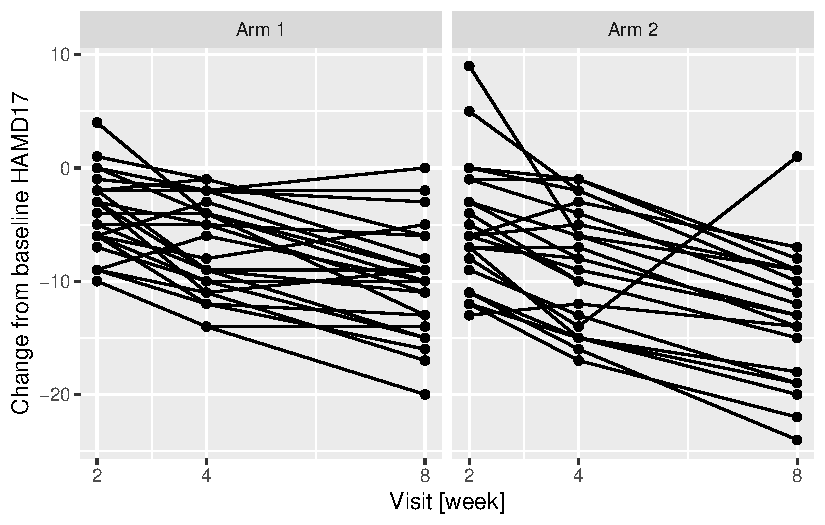
\includegraphics{s1_visualization_files/figure-pdf/fig-traj-1.pdf}

}

\caption{\label{fig-traj}Individual trajectories of HAMD17 by treatment
group}

\end{figure}

Figure: Mean change from baseline for each treatment group

\begin{Shaded}
\begin{Highlighting}[]
\FunctionTok{ggplot}\NormalTok{(}\AttributeTok{data =}\NormalTok{ all2, }\FunctionTok{aes}\NormalTok{(}\AttributeTok{x =}\NormalTok{ week, }\AttributeTok{y =}\NormalTok{ change)) }\SpecialCharTok{+}  
  \FunctionTok{geom\_point}\NormalTok{(}\FunctionTok{aes}\NormalTok{(}\AttributeTok{colour=}\FunctionTok{factor}\NormalTok{(group))) }\SpecialCharTok{+} \FunctionTok{ylab}\NormalTok{(}\StringTok{"Change from baseline HAMD17"}\NormalTok{) }\SpecialCharTok{+}
  \FunctionTok{scale\_x\_continuous}\NormalTok{(}\AttributeTok{name=}\StringTok{"Visit [week]"}\NormalTok{, }\AttributeTok{breaks=}\FunctionTok{c}\NormalTok{(}\DecValTok{2}\NormalTok{,}\DecValTok{4}\NormalTok{,}\DecValTok{8}\NormalTok{)) }\SpecialCharTok{+}
  \FunctionTok{stat\_summary}\NormalTok{(}\FunctionTok{aes}\NormalTok{(}\AttributeTok{group =}\NormalTok{ group, }\AttributeTok{colour=}\FunctionTok{factor}\NormalTok{(group)), }\AttributeTok{geom =} \StringTok{"line"}\NormalTok{, }\AttributeTok{fun.y =}\NormalTok{ mean,}
               \AttributeTok{size =} \DecValTok{1}\NormalTok{) }\SpecialCharTok{+}
  \FunctionTok{stat\_summary}\NormalTok{(}\FunctionTok{aes}\NormalTok{(}\AttributeTok{group =}\NormalTok{ group, }\AttributeTok{colour=}\FunctionTok{factor}\NormalTok{(group)), }\AttributeTok{geom =} \StringTok{"point"}\NormalTok{, }\AttributeTok{fun.y =}\NormalTok{ mean,}
               \AttributeTok{shape=}\DecValTok{17}\NormalTok{,}\AttributeTok{size =} \DecValTok{2}\NormalTok{)}
\end{Highlighting}
\end{Shaded}

\begin{figure}[H]

{\centering 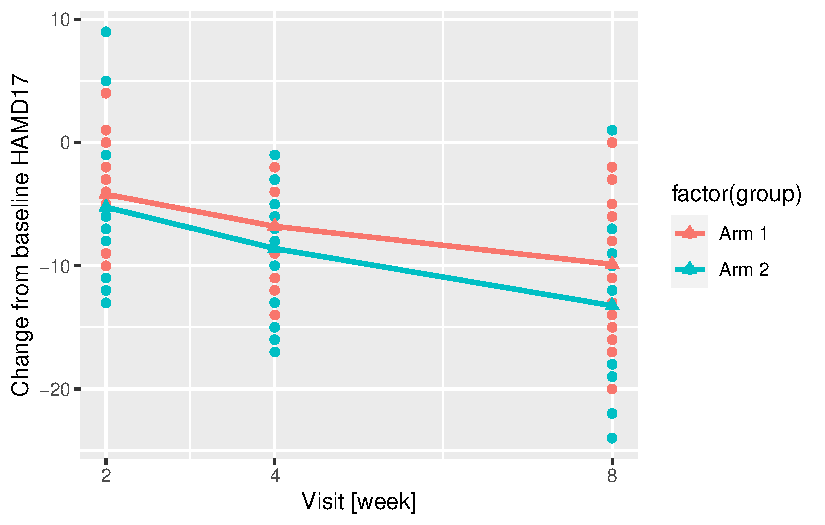
\includegraphics{s1_visualization_files/figure-pdf/fig-mean-1.pdf}

}

\caption{\label{fig-mean}Mean HAMD17 change from baseline by treatment
group}

\end{figure}

Frequency for sex per treatment group

\begin{Shaded}
\begin{Highlighting}[]
\NormalTok{all2 }\SpecialCharTok{\%\textgreater{}\%} \FunctionTok{filter}\NormalTok{(time}\SpecialCharTok{==}\DecValTok{1}\NormalTok{) }\SpecialCharTok{\%\textgreater{}\%}
  \FunctionTok{tbl\_summary}\NormalTok{(}
    \AttributeTok{include =} \FunctionTok{c}\NormalTok{(gender),}
    \AttributeTok{by =}\NormalTok{ group}
\NormalTok{  )}
\end{Highlighting}
\end{Shaded}

\begin{longtable}[]{@{}lcc@{}}
\toprule\noalign{}
\textbf{Characteristic} & \textbf{Arm 1}, N = 25 & \textbf{Arm 2}, N =
25 \\
\midrule\noalign{}
\endhead
\bottomrule\noalign{}
\endlastfoot
PATIENT SEX & & \\
F & 10 (40\%) & 19 (76\%) \\
M & 15 (60\%) & 6 (24\%) \\
\end{longtable}

Figure: Mean change from baseline stratified by sex

\begin{Shaded}
\begin{Highlighting}[]
\FunctionTok{ggplot}\NormalTok{(}\AttributeTok{data =}\NormalTok{ all2, }\FunctionTok{aes}\NormalTok{(}\AttributeTok{x =}\NormalTok{ week, }\AttributeTok{y =}\NormalTok{ change)) }\SpecialCharTok{+}  \FunctionTok{facet\_grid}\NormalTok{(.}\SpecialCharTok{\textasciitilde{}}\NormalTok{gender) }\SpecialCharTok{+}
  \FunctionTok{geom\_point}\NormalTok{(}\FunctionTok{aes}\NormalTok{(}\AttributeTok{colour=}\FunctionTok{factor}\NormalTok{(group))) }\SpecialCharTok{+} \FunctionTok{ylab}\NormalTok{(}\StringTok{"Change from baseline HAMD17"}\NormalTok{) }\SpecialCharTok{+}
  \FunctionTok{scale\_x\_continuous}\NormalTok{(}\AttributeTok{name=}\StringTok{"Visit [week]"}\NormalTok{, }\AttributeTok{breaks=}\FunctionTok{c}\NormalTok{(}\DecValTok{2}\NormalTok{,}\DecValTok{4}\NormalTok{,}\DecValTok{8}\NormalTok{)) }\SpecialCharTok{+}
  \FunctionTok{stat\_summary}\NormalTok{(}\FunctionTok{aes}\NormalTok{(}\AttributeTok{group =}\NormalTok{ group, }\AttributeTok{colour=}\FunctionTok{factor}\NormalTok{(group)), }\AttributeTok{geom =} \StringTok{"line"}\NormalTok{, }\AttributeTok{fun.y =}\NormalTok{ mean,}
               \AttributeTok{size =} \DecValTok{1}\NormalTok{) }\SpecialCharTok{+}
  \FunctionTok{stat\_summary}\NormalTok{(}\FunctionTok{aes}\NormalTok{(}\AttributeTok{group =}\NormalTok{ group, }\AttributeTok{colour=}\FunctionTok{factor}\NormalTok{(group)), }\AttributeTok{geom =} \StringTok{"point"}\NormalTok{, }\AttributeTok{fun.y =}\NormalTok{ mean,}
               \AttributeTok{shape=}\DecValTok{17}\NormalTok{,}\AttributeTok{size =} \DecValTok{2}\NormalTok{)}
\end{Highlighting}
\end{Shaded}

\begin{figure}[H]

{\centering 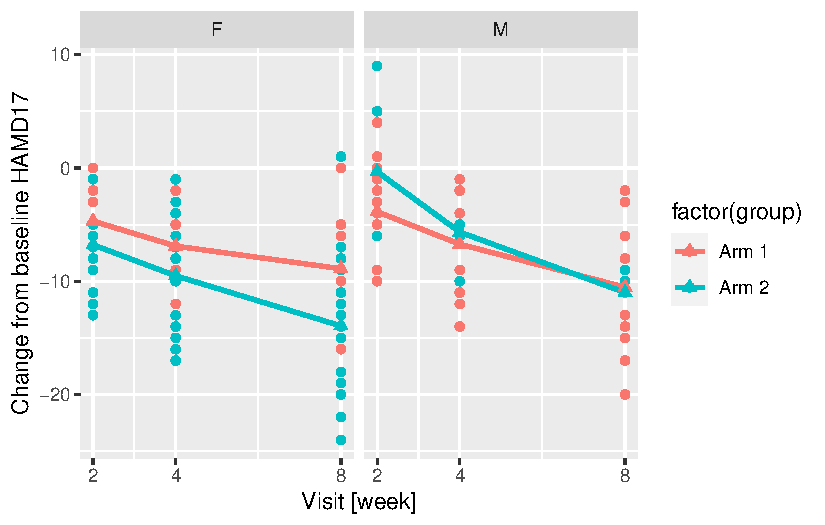
\includegraphics{s1_visualization_files/figure-pdf/fig-meansex-1.pdf}

}

\caption{\label{fig-meansex}Mean HAMD17 change from baseline by
treatment group stratified by sex}

\end{figure}

\hypertarget{data-set-all2-with-drop-out}{%
\subsection{Data set all2 with
drop-out}\label{data-set-all2-with-drop-out}}

\begin{itemize}
\tightlist
\item
  2nd version = missing data: identical to the first except some data
  were missing (drop-out), variable \emph{chgdrop}
\item
  This version is later relevant when considering missing data. Thus,
  have a short look at the data.
\end{itemize}

Table: Summary statistics for HAMD17 by treatment and week in the all2
data set with drop-outs

\begin{Shaded}
\begin{Highlighting}[]
\NormalTok{all2 }\SpecialCharTok{\%\textgreater{}\%}
  \FunctionTok{select}\NormalTok{(chgdrop, group, avisit) }\SpecialCharTok{\%\textgreater{}\%}
  \FunctionTok{tbl\_strata}\NormalTok{(}\AttributeTok{strata=}\NormalTok{group, }
             \SpecialCharTok{\textasciitilde{}}\NormalTok{.x }\SpecialCharTok{\%\textgreater{}\%} 
               \FunctionTok{tbl\_summary}\NormalTok{(}\AttributeTok{by =}\NormalTok{ avisit,}
                           \AttributeTok{statistic =} \FunctionTok{list}\NormalTok{(}
      \FunctionTok{all\_continuous}\NormalTok{() }\SpecialCharTok{\textasciitilde{}} \StringTok{"\{mean\} (\{sd\})"}\NormalTok{), }
      \AttributeTok{digits =} \FunctionTok{all\_continuous}\NormalTok{() }\SpecialCharTok{\textasciitilde{}} \DecValTok{2}\NormalTok{ ) }\SpecialCharTok{\%\textgreater{}\%}
      \FunctionTok{modify\_header}\NormalTok{(}\AttributeTok{label =} \StringTok{"**Variable**"}\NormalTok{)}
\NormalTok{)}
\end{Highlighting}
\end{Shaded}

\begin{longtable}[]{@{}
  >{\raggedright\arraybackslash}p{(\columnwidth - 12\tabcolsep) * \real{0.0977}}
  >{\centering\arraybackslash}p{(\columnwidth - 12\tabcolsep) * \real{0.1504}}
  >{\centering\arraybackslash}p{(\columnwidth - 12\tabcolsep) * \real{0.1504}}
  >{\centering\arraybackslash}p{(\columnwidth - 12\tabcolsep) * \real{0.1504}}
  >{\centering\arraybackslash}p{(\columnwidth - 12\tabcolsep) * \real{0.1504}}
  >{\centering\arraybackslash}p{(\columnwidth - 12\tabcolsep) * \real{0.1504}}
  >{\centering\arraybackslash}p{(\columnwidth - 12\tabcolsep) * \real{0.1504}}@{}}
\toprule\noalign{}
\begin{minipage}[b]{\linewidth}\raggedright
\textbf{Variable}
\end{minipage} & \begin{minipage}[b]{\linewidth}\centering
\textbf{Week 2}, N = 25
\end{minipage} & \begin{minipage}[b]{\linewidth}\centering
\textbf{Week 4}, N = 25
\end{minipage} & \begin{minipage}[b]{\linewidth}\centering
\textbf{Week 8}, N = 25
\end{minipage} & \begin{minipage}[b]{\linewidth}\centering
\textbf{Week 2}, N = 25
\end{minipage} & \begin{minipage}[b]{\linewidth}\centering
\textbf{Week 4}, N = 25
\end{minipage} & \begin{minipage}[b]{\linewidth}\centering
\textbf{Week 8}, N = 25
\end{minipage} \\
\midrule\noalign{}
\endhead
\bottomrule\noalign{}
\endlastfoot
chgdrop & -4.20 (3.66) & -6.80 (4.63) & -10.17 (4.88) & -5.24 (5.49) &
-8.14 (5.27) & -13.11 (5.44) \\
Unknown & 0 & 5 & 7 & 0 & 3 & 6 \\
\end{longtable}

\hypertarget{data-set-high2}{%
\section{Data set high2}\label{data-set-high2}}

\begin{itemize}
\tightlist
\item
  Large data set with n=100 subjects.
\item
  Note that we have no intermittent missing values but drop-outs.
\end{itemize}

Looking at the variables in the data set.

\begin{Shaded}
\begin{Highlighting}[]
\FunctionTok{head}\NormalTok{(high2)}
\end{Highlighting}
\end{Shaded}

\begin{verbatim}
# A tibble: 6 x 16
# Groups:   patient [2]
  patient trt   poolinv basval  week change pgiimp   age gender  drop .groups
    <dbl> <chr> <chr>    <dbl> <dbl>  <dbl>  <dbl> <dbl> <chr>  <dbl> <chr>  
1    1401 1     005         19     1     -7      3  44.5 F          2 drop   
2    1401 1     005         19     2     -4      3  44.5 F          2 drop   
3    1411 2     005         17     1      0      3  35.7 F          8 drop   
4    1411 2     005         17     2     -2      3  35.7 F          8 drop   
5    1411 2     005         17     4      2      3  35.7 F          8 drop   
6    1411 2     005         17     6     -3      2  35.7 F          8 drop   
# i 5 more variables: aval <dbl>, group <fct>, avisit <fct>, dropout_grp <fct>,
#   subject <fct>
\end{verbatim}

\hypertarget{task-2---exploration-of-data-set-high2---15-minutes-working-time}{%
\subsection{Task 2 - Exploration of data set high2 - 15 minutes working
time}\label{task-2---exploration-of-data-set-high2---15-minutes-working-time}}

\begin{itemize}
\tightlist
\item
  Explore the drop-outs e.g.~number of observations by week.
\item
  Summary statistics for HAMD17 change.
\item
  Generate and interpret the group-wise boxplots of the change from
  baseline.
\item
  Mean change from baseline for different drop-out groups (by
  treatment). Comment on the plot.
\end{itemize}

\hypertarget{task-2-discussion-possible-solution}{%
\subsection{Task 2 Discussion, possible
solution}\label{task-2-discussion-possible-solution}}

Table: Summary statistics for HAMD17 by treatment and week in the high2
data set

\begin{Shaded}
\begin{Highlighting}[]
\NormalTok{high2 }\SpecialCharTok{\%\textgreater{}\%} \FunctionTok{ungroup}\NormalTok{() }\SpecialCharTok{\%\textgreater{}\%}
  \FunctionTok{select}\NormalTok{(change, group, avisit) }\SpecialCharTok{\%\textgreater{}\%}
  \FunctionTok{tbl\_strata}\NormalTok{(}\AttributeTok{strata=}\NormalTok{group, }
             \SpecialCharTok{\textasciitilde{}}\NormalTok{.x }\SpecialCharTok{\%\textgreater{}\%} 
               \FunctionTok{tbl\_summary}\NormalTok{(}\AttributeTok{by =}\NormalTok{ avisit,}
                           \AttributeTok{statistic =} \FunctionTok{list}\NormalTok{(}
                             \FunctionTok{all\_continuous}\NormalTok{() }\SpecialCharTok{\textasciitilde{}} \StringTok{"\{mean\} (\{sd\})"}\NormalTok{), }
                           \AttributeTok{digits =} \FunctionTok{all\_continuous}\NormalTok{() }\SpecialCharTok{\textasciitilde{}} \DecValTok{2}\NormalTok{ ) }\SpecialCharTok{\%\textgreater{}\%}
                \FunctionTok{modify\_header}\NormalTok{(}\AttributeTok{label =} \StringTok{"**Variable**"}\NormalTok{)}
\NormalTok{  )}
\end{Highlighting}
\end{Shaded}

\begin{longtable}[]{@{}
  >{\raggedright\arraybackslash}p{(\columnwidth - 20\tabcolsep) * \real{0.0605}}
  >{\centering\arraybackslash}p{(\columnwidth - 20\tabcolsep) * \real{0.0977}}
  >{\centering\arraybackslash}p{(\columnwidth - 20\tabcolsep) * \real{0.0930}}
  >{\centering\arraybackslash}p{(\columnwidth - 20\tabcolsep) * \real{0.0930}}
  >{\centering\arraybackslash}p{(\columnwidth - 20\tabcolsep) * \real{0.0930}}
  >{\centering\arraybackslash}p{(\columnwidth - 20\tabcolsep) * \real{0.0930}}
  >{\centering\arraybackslash}p{(\columnwidth - 20\tabcolsep) * \real{0.0977}}
  >{\centering\arraybackslash}p{(\columnwidth - 20\tabcolsep) * \real{0.0930}}
  >{\centering\arraybackslash}p{(\columnwidth - 20\tabcolsep) * \real{0.0930}}
  >{\centering\arraybackslash}p{(\columnwidth - 20\tabcolsep) * \real{0.0930}}
  >{\centering\arraybackslash}p{(\columnwidth - 20\tabcolsep) * \real{0.0930}}@{}}
\toprule\noalign{}
\begin{minipage}[b]{\linewidth}\raggedright
\textbf{Variable}
\end{minipage} & \begin{minipage}[b]{\linewidth}\centering
\textbf{Week 1}, N = 100
\end{minipage} & \begin{minipage}[b]{\linewidth}\centering
\textbf{Week 2}, N = 92
\end{minipage} & \begin{minipage}[b]{\linewidth}\centering
\textbf{Week 4}, N = 85
\end{minipage} & \begin{minipage}[b]{\linewidth}\centering
\textbf{Week 6}, N = 73
\end{minipage} & \begin{minipage}[b]{\linewidth}\centering
\textbf{Week 8}, N = 60
\end{minipage} & \begin{minipage}[b]{\linewidth}\centering
\textbf{Week 1}, N = 100
\end{minipage} & \begin{minipage}[b]{\linewidth}\centering
\textbf{Week 2}, N = 90
\end{minipage} & \begin{minipage}[b]{\linewidth}\centering
\textbf{Week 4}, N = 85
\end{minipage} & \begin{minipage}[b]{\linewidth}\centering
\textbf{Week 6}, N = 75
\end{minipage} & \begin{minipage}[b]{\linewidth}\centering
\textbf{Week 8}, N = 70
\end{minipage} \\
\midrule\noalign{}
\endhead
\bottomrule\noalign{}
\endlastfoot
change & -1.49 (3.91) & -3.16 (5.69) & -4.51 (6.23) & -5.51 (6.16) &
-6.58 (5.99) & -1.84 (5.58) & -4.30 (6.82) & -6.47 (6.84) & -8.29 (6.96)
& -8.99 (7.04) \\
\end{longtable}

Figure: Distribution of HAMD17 change from baseline

\begin{Shaded}
\begin{Highlighting}[]
\FunctionTok{ggplot}\NormalTok{(}\AttributeTok{data =}\NormalTok{ high2, }\FunctionTok{aes}\NormalTok{(}\AttributeTok{x =}\NormalTok{ avisit, }\AttributeTok{y =}\NormalTok{ change, }\AttributeTok{fill=}\NormalTok{group)) }\SpecialCharTok{+} 
  \FunctionTok{geom\_boxplot}\NormalTok{() }\SpecialCharTok{+} \FunctionTok{ylab}\NormalTok{(}\StringTok{"Change from baseline HAMD17"}\NormalTok{) }\SpecialCharTok{+} \FunctionTok{xlab}\NormalTok{(}\StringTok{"Visit"}\NormalTok{)}
\end{Highlighting}
\end{Shaded}

\begin{figure}[H]

{\centering 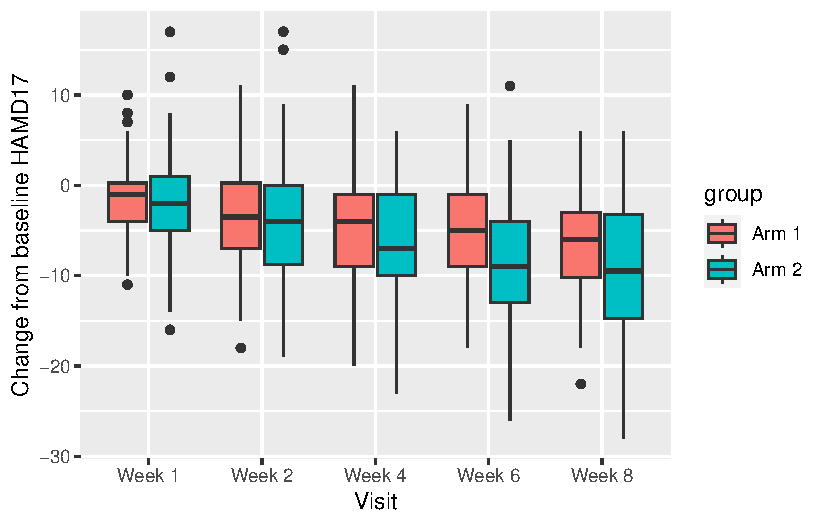
\includegraphics{s1_visualization_files/figure-pdf/fig-box-1.pdf}

}

\caption{\label{fig-box}Distribution of HAMD17 change from baseline by
treatment group at each visit}

\end{figure}

Figure: Mean HAMD17 changes by drop-out group

\begin{Shaded}
\begin{Highlighting}[]
\FunctionTok{ggplot}\NormalTok{(}\AttributeTok{data =}\NormalTok{ high2, }\FunctionTok{aes}\NormalTok{(}\AttributeTok{x =}\NormalTok{ week, }\AttributeTok{y =}\NormalTok{ change, }\AttributeTok{group=}\NormalTok{patient)) }\SpecialCharTok{+} 
  \FunctionTok{geom\_point}\NormalTok{(}\AttributeTok{col=}\StringTok{"lightgray"}\NormalTok{) }\SpecialCharTok{+} \FunctionTok{geom\_line}\NormalTok{(}\AttributeTok{col=}\StringTok{"lightgray"}\NormalTok{) }\SpecialCharTok{+} \FunctionTok{facet\_grid}\NormalTok{(.}\SpecialCharTok{\textasciitilde{}}\NormalTok{group) }\SpecialCharTok{+}
  \FunctionTok{ylab}\NormalTok{(}\StringTok{"Change from baseline HAMD17"}\NormalTok{) }\SpecialCharTok{+} \FunctionTok{scale\_x\_continuous}\NormalTok{(}\AttributeTok{name=}\StringTok{"Visit [week]"}\NormalTok{, }\AttributeTok{breaks=}\FunctionTok{c}\NormalTok{(}\DecValTok{1}\NormalTok{,}\DecValTok{2}\NormalTok{,}\DecValTok{4}\NormalTok{,}\DecValTok{6}\NormalTok{,}\DecValTok{8}\NormalTok{)) }\SpecialCharTok{+}
  \FunctionTok{stat\_summary}\NormalTok{(}\FunctionTok{aes}\NormalTok{(}\AttributeTok{group =}\NormalTok{ dropout\_grp, }\AttributeTok{colour=}\FunctionTok{factor}\NormalTok{(dropout\_grp)), }\AttributeTok{geom =} \StringTok{"line"}\NormalTok{, }\AttributeTok{fun.y =}\NormalTok{ mean,}
               \AttributeTok{size =} \DecValTok{1}\NormalTok{) }\SpecialCharTok{+}
  \FunctionTok{stat\_summary}\NormalTok{(}\FunctionTok{aes}\NormalTok{(}\AttributeTok{group =}\NormalTok{ dropout\_grp, }\AttributeTok{colour=}\FunctionTok{factor}\NormalTok{(dropout\_grp)), }\AttributeTok{geom =} \StringTok{"point"}\NormalTok{, }\AttributeTok{fun.y =}\NormalTok{ mean,}
               \AttributeTok{shape=}\DecValTok{17}\NormalTok{,}\AttributeTok{size =} \DecValTok{2}\NormalTok{)}
\end{Highlighting}
\end{Shaded}

\begin{figure}[H]

{\centering 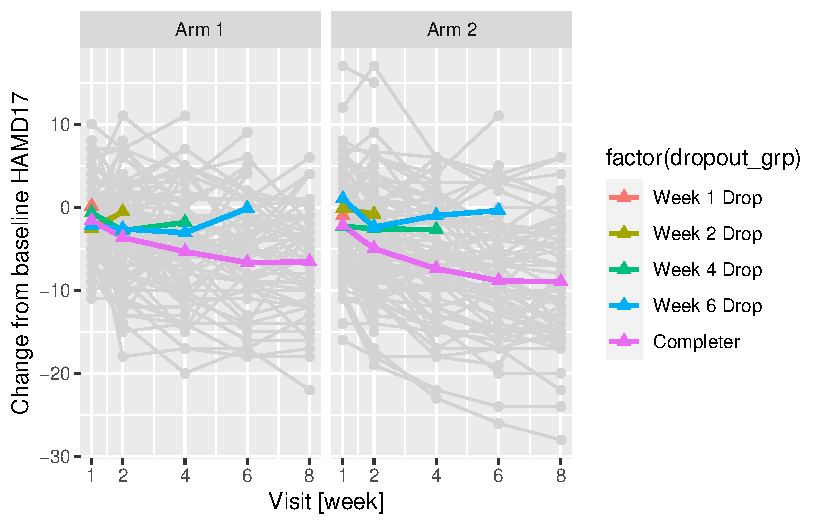
\includegraphics{s1_visualization_files/figure-pdf/fig-traj2-1.pdf}

}

\caption{\label{fig-traj2}Visit-wise mean HAMD17 changes from baseline
by treatment group and drop-out}

\end{figure}

\bookmarksetup{startatroot}

\hypertarget{correlation-structure-covariance-matrices}{%
\chapter{Correlation structure, covariance
matrices}\label{correlation-structure-covariance-matrices}}

\begin{itemize}
\tightlist
\item
  Longitudinal data allows to exploit the correlation between otucomes
  wihtin subjects regardless of whether or not focues is on a single
  landmark time point.
\item
  Model within-subject error correlation
\item
  Different residual covariance structures can be implemented
\end{itemize}

\hypertarget{overview---different-covariance-matrices}{%
\section{Overview - different covariance
matrices}\label{overview---different-covariance-matrices}}

\begin{itemize}
\tightlist
\item
  Variance components (VC) independence structure
\item
  Compound symmetry (CS) also known as exchangeable
\item
  Toeplitz (TOEP)
\item
  First order auto regressive (AR(1))
\item
  Unstructured (UN)
\end{itemize}

Selected covariance structures for data with three assessment times
(t=3) are shown below. Note that with three assessment times, the number
of parameters estimated for the various structures did not differ as
much as would be the case with more assessment times. Thus, results from
different covariance structures are more similar than would be the case
with more assessment times.

\hypertarget{independence-structure-vc}{%
\subsection{Independence structure
(VC)}\label{independence-structure-vc}}

Constant variance. It is assumed to be no correlation between
assessments (residuals are independent across time).
\[ R = \begin{bmatrix}
   \sigma^2   & 0  & 0  \\
   0  & \sigma^2   & 0 \\
   0  & 0  & \sigma^2
   \end{bmatrix}\]

\hypertarget{compound-symmetry-cs}{%
\subsection{Compound symmetry (CS)}\label{compound-symmetry-cs}}

Constant variance and constant covariance across all assessments. Also
known as exchangeable. It requires two parameter estimates. Most
simplest repeated measures (i.e., correlated errors) structure.

\[ R = \begin{bmatrix}
   \sigma^2 + \sigma_1 & \sigma_1  & \sigma_1  \\
   \sigma_1  & \sigma^2 + \sigma_1  & \sigma_1  \\
   \sigma_1  & \sigma_1  & \sigma^2 + \sigma_1
   \end{bmatrix}\]

\hypertarget{unstructured-un}{%
\subsection{Unstructured (UN)}\label{unstructured-un}}

This is the most general (saturated) model. It has t + {[}t(t-1)/2{]}
parameters to be estimated. Here it is 3 + 3 = 6 parameters.

\[ R = \begin{bmatrix}
   \sigma_1^2 & \sigma_{21}  & \sigma_{31}  \\
   \sigma_{21}  & \sigma_2^2   & \sigma_{32}  \\
   \sigma_{31}  & \sigma_{32}  & \sigma_3^2
   \end{bmatrix}\]

\hypertarget{toeplitz-structure-toep}{%
\subsection{Toeplitz structure (TOEP)}\label{toeplitz-structure-toep}}

Homogenous variances and heterogenous correlations. Same correlation
value is used whenever the degree of adjacency is the same
e.g.~correlation between times 1 and 2 = correlation between times 2 and
3. Repeated measurements are assumed to be equally spaced. TOEP requries
t parameter estimates so here we have t=3 parameter.

\[ R = \begin{bmatrix}
   \sigma^2  & \sigma_1^2 & \sigma_2^2 \  \\
   \sigma_1^2 & \sigma^2  & \sigma_1^2  \\
   \sigma_2^2  & \sigma_1^2 & \sigma^2 
   \end{bmatrix}\]

\hypertarget{autoregressive-structure-ar1}{%
\subsection{Autoregressive structure
(AR(1))}\label{autoregressive-structure-ar1}}

Correlation decreases as time between observations increases. Assumtpion
of equal spacing between each repeated measurement must be reasonably
applicable. This structure requires the estimation of two parameters.

\[ R = \begin{bmatrix}
   \sigma^2  & \sigma^2 \rho  & \sigma^2 \rho^2  \\
   \sigma^2 \rho & \sigma^2   & \sigma^2 \rho  \\
  \sigma^2 \rho^2  & \sigma^2 \rho  & \sigma^2 
   \end{bmatrix}\]

\hypertarget{spatial-power-sp}{%
\subsection{Spatial Power (SP)}\label{spatial-power-sp}}

Spatial covariance structures does not require equal spacing between
measurements. Instead, as long as the distance between visits can be
quantified in terms of time and/or other coordinates, the spatial
covariance structure can be applied. Covariances are mathematical
functions of Euclidean distances between observed measurements. Again,
two parameters need to be estimated.

For spatial exponential, the covariance structure is defined as follows:

\[ R = \begin{bmatrix}
   \sigma^2  & \sigma^2 \rho_{12}  & \sigma^2 \rho_{13}  \\
   \sigma^2 \rho_{21} & \sigma^2   & \sigma^2 \rho_{23}  \\
  \sigma^2 \rho_{31}  & \sigma^2 \rho_{32}  & \sigma^2 
   \end{bmatrix}\]

with \[ \rho_{ij}=\rho^{d_{ij}} \] where \[d_{ij} \] is the distance
between time point i and time point j e.g.~distance in weeks.

\hypertarget{selecting-the-covariance-structure}{%
\section{Selecting the covariance
structure}\label{selecting-the-covariance-structure}}

There are a variety of considerations when selecting the covariance
structure: - number of parameters - interpretation of the structure -
model fit

UN is the most flexible (complex) structure and can fail to run
especially if one has many repeated measures. Choose a reasonable
covaraiance structure which is the best compromise between model fit and
complexity. E.g. use AIC as it penalises more complex models.

\hypertarget{task-3---exploration-of-correlation-in-the-data}{%
\section{Task 3 - Exploration of correlation in the
data}\label{task-3---exploration-of-correlation-in-the-data}}

\begin{itemize}
\tightlist
\item
  Compute the empirical correlations between measurement timepoints in
  the all2 data set (e.g.~correlation between baseline and post-baseline
  changes).
\item
  Looking at these correlations + using your knowledge of the experiment
  (e.g., spacing of measurements), comment on the suitability of the
  correlation structures VC, CS, UN, AR(1).
\end{itemize}

\hypertarget{task-3---discussion-and-possible-solution}{%
\section{Task 3 - Discussion and possible
solution}\label{task-3---discussion-and-possible-solution}}

Table: Correlation and covariance matrix

\begin{Shaded}
\begin{Highlighting}[]
\NormalTok{all2.w }\OtherTok{\textless{}{-}}\NormalTok{ all2 }\SpecialCharTok{\%\textgreater{}\%} 
  \FunctionTok{pivot\_wider}\NormalTok{(}\AttributeTok{id\_cols=}\NormalTok{subject,}\AttributeTok{names\_from =}\NormalTok{ time, }\AttributeTok{values\_from =} \FunctionTok{c}\NormalTok{(basval,change)) }\SpecialCharTok{\%\textgreater{}\%} 
  \FunctionTok{select}\NormalTok{(}\SpecialCharTok{{-}}\FunctionTok{c}\NormalTok{(basval\_2,basval\_3))}

\FunctionTok{cor}\NormalTok{(all2.w[}\SpecialCharTok{{-}}\DecValTok{1}\NormalTok{]) }
\end{Highlighting}
\end{Shaded}

\begin{verbatim}
            basval_1   change_1   change_2    change_3
basval_1  1.00000000 -0.2636447 -0.3165711 -0.02915138
change_1 -0.26364471  1.0000000  0.7557078  0.51502724
change_2 -0.31657106  0.7557078  1.0000000  0.71298768
change_3 -0.02915138  0.5150272  0.7129877  1.00000000
\end{verbatim}

\begin{Shaded}
\begin{Highlighting}[]
\FunctionTok{cov}\NormalTok{(all2.w[}\SpecialCharTok{{-}}\DecValTok{1}\NormalTok{])}
\end{Highlighting}
\end{Shaded}

\begin{verbatim}
           basval_1  change_1  change_2   change_3
basval_1 16.3330612 -4.955918 -6.253061 -0.6391837
change_1 -4.9559184 21.634286 17.179592 12.9967347
change_2 -6.2530612 17.179592 23.887755 18.9061224
change_3 -0.6391837 12.996735 18.906122 29.4351020
\end{verbatim}

\hypertarget{taking-a-step-back-consequences-of-ignoring-correlation-among-longitudinal-data}{%
\section{Taking a step back: Consequences of Ignoring Correlation among
Longitudinal
Data}\label{taking-a-step-back-consequences-of-ignoring-correlation-among-longitudinal-data}}

This technical detour is motivated by (Fitzmaurice 2011). Let us assume
we are only interested in the first two responses in a clinical study,
say Visit 1 (Baseline) and Visit 2. Out interest lies in an assessment
of mean changes over time (for the sake of simplicity in a single
treatment group only), i.e.~we wish to estimate

\[
\hat\delta := \hat\mu_2 - \hat\mu_1 = \frac{1}{N} \sum_{i=1}^N (Y_{i2} - Y_{i1})\,,
\]

where \(Y_{i1}\) and \(Y_{i2}\) are observations from subject \(i\) at
Visit 1 and Visit 2, respectively. To obtain the standard error (SE) and
get a notion of variability, we compute the variance of \(\hat\delta\)
and see that

\[
\text{Var}(\hat\delta) = \text{Var}\left(\frac{1}{N} \sum_{i=1}^N (Y_{i2} - Y_{i1})\right) = \frac{1}{N} (\sigma_1^2 + \sigma_2^2 - 2\sigma_{12})\,.
\]

The inclusion of the term \(- 2\sigma_{12}\) accounts for the
correlation between responses at Visit 1 and Visit 2. As data from
adjacent visits is usually positively correlated, the omission of the
correlation term leads to an overestimation of the variance and thus the
SE associated with the treatment effect.

\bookmarksetup{startatroot}

\hypertarget{inference-from-longitudinal-data}{%
\chapter{Inference from Longitudinal
Data}\label{inference-from-longitudinal-data}}

This section will focus on the application of Mixed Model with Repeated
Measures (MMRMs). Our main focus will be the modeling of the means of
the data. MMRMs are generalizations of standard linear models in the way
that data is allowed to be correlated between subsequent measurements
from the same subject and exhibit non-constant variability. A nice
summary can be found in the user manual for the MIXED Procedure
\href{https://support.sas.com/documentation/cdl/en/statug/63033/HTML/default/viewer.htm\#mixed_toc.htm}{SAS},
or the
\href{https://openpharma.github.io/mmrm/latest-tag/articles/methodological_introduction.html}{vignette}
for the \texttt{mmrm} package (Sabanes Bove et al. 2024).

The primary assumptions for MMRMs are:

\begin{itemize}
\item
  The data are normally distributed
\item
  The means (expected values) of the data are linear in terms of a
  certain set of parameters.
\item
  The variances and covariances of the data are in terms of a different
  set of parameters, and they exhibit a structure matching one of those
  outlined in the former chapter.
\end{itemize}

The mixed linear model can be described via the following formula

\[
y_i = X_i\beta\,+\,Z_i\gamma_i\,+\,\varepsilon_i\,,\, i = 1,\ldots,N
\]

where \(y\) is the vector of responses (observed data, dependent
variable), \(\beta\) is an unknown vector of fixed effects with known
design matrix \(X\), \(\gamma\) is an unknown vector of random effects
with known design matrix \(Z\), and \(\varepsilon\) is an unknown random
error vector. Furthermore \(N\) denotes the total number of subjects in
our analysis. For the sake of readability, we will omit the subject
index and simplify the above formula to

\[
y = X\beta\,+\,Z\gamma\,+\,\varepsilon\,.
\]

We will further assume that \(\gamma\) and \(\varepsilon\) are
uncorrelated Gaussian random variables with expectation \(0\) and
variances \(G\) and \(R\), respectively. Then the variance-covariance
matrix of \(y\) is given by

\[
\text{Var}(y) := V = ZGZ' + R\,.
\] In this case \(ZGZ'\) comprises the random effects component, and
\(R\) is the within-subject component.

In this workshop we will focus on the case where only the within-subject
component is accounted for, via modeling of the \(R\) matrix. The random
effects component \(Z\gamma\) will be omitted. In this case we will have
\(\text{Var}(y) = V = R\), resulting in a model given by

\[
y = X\beta\,+\,\varepsilon\,.
\]

\hypertarget{categorical-time}{%
\section{Categorical Time}\label{categorical-time}}

In the following sections we will use the package \texttt{mmrm} (Sabanes
Bove et al. 2024). You can start and familiarise yourself with the main
function \texttt{mmrm()} using the command

\begin{Shaded}
\begin{Highlighting}[]
\FunctionTok{library}\NormalTok{(mmrm)}
\NormalTok{?mmrm}
\end{Highlighting}
\end{Shaded}

Two inputs are strictly required to get \texttt{mmrm()} to work:

\begin{itemize}
\item
  A model formula
\item
  The dataset, containing the response, as well as all fixed effects and
  variables in the covariance matrix.
\end{itemize}

\textbf{Exercise}: Fit a model \texttt{fit\_cat\_time} using the dataset
\texttt{all2}, with change as dependent variable, baseline value, visit,
baseline by visit interaction and treatment by visit interaction as
fixed effects and an unstructured covariance matrix for visits within
each subject.

\begin{itemize}
\item
  How do different choices for covariance matrices change the results?
  What is the difference on the estimation procedure?
\item
  You can obtain a summary of the fit results via
  \texttt{summary(fit\_cat\_time)}. How do you interpret the fit
  summary?
\item
  Look at the structure of the fit summary and try to extract the
  estimate of the \(R\) matrix.
\item
  How do other choices of covariance structures influence the
  estimation?
\end{itemize}

\hypertarget{unstructured-us}{%
\subsection{Unstructured (US)}\label{unstructured-us}}

Unstructured corresponds to a saturated variance-covariance matrix and
involves the estimation of \(m\,(m+1)/2\) variance components, where
\(m\) is the number of follow-up visits. In our case, we can see that a
total of 6 variance parameters were estimated.

\begin{Shaded}
\begin{Highlighting}[]
\NormalTok{fit\_cat\_time }\OtherTok{\textless{}{-}}\NormalTok{ mmrm}\SpecialCharTok{::}\FunctionTok{mmrm}\NormalTok{(}
  \AttributeTok{formula =}\NormalTok{ change }\SpecialCharTok{\textasciitilde{}}\NormalTok{ basval}\SpecialCharTok{*}\NormalTok{avisit }\SpecialCharTok{+}\NormalTok{ trt}\SpecialCharTok{*}\NormalTok{avisit }\SpecialCharTok{+} \FunctionTok{us}\NormalTok{(avisit }\SpecialCharTok{|}\NormalTok{ subject),}
  \AttributeTok{data =}\NormalTok{ all2,}
  \AttributeTok{control =} \FunctionTok{mmrm\_control}\NormalTok{(}\AttributeTok{method =} \StringTok{"Kenward{-}Roger"}\NormalTok{)}
\NormalTok{)}

\FunctionTok{summary}\NormalTok{(fit\_cat\_time)}
\end{Highlighting}
\end{Shaded}

\begin{verbatim}
mmrm fit

Formula:     change ~ basval * avisit + trt * avisit + us(avisit | subject)
Data:        all2 (used 150 observations from 50 subjects with maximum 3 
timepoints)
Covariance:  unstructured (6 variance parameters)
Method:      Kenward-Roger
Vcov Method: Kenward-Roger
Inference:   REML

Model selection criteria:
     AIC      BIC   logLik deviance 
   822.4    833.9   -405.2    810.4 

Coefficients: 
                     Estimate Std. Error        df t value Pr(>|t|)   
(Intercept)           1.98452    3.27479  47.00000   0.606  0.54743   
basval               -0.31235    0.15905  47.00000  -1.964  0.05548 . 
avisitWeek 4         -0.90862    2.39866  47.00000  -0.379  0.70654   
avisitWeek 8        -10.58630    3.45922  47.00000  -3.060  0.00365 **
trt2                 -1.18993    1.27265  47.00000  -0.935  0.35457   
basval:avisitWeek 4  -0.08542    0.11650  47.00000  -0.733  0.46704   
basval:avisitWeek 8   0.24779    0.16801  47.00000   1.475  0.14691   
avisitWeek 4:trt2    -0.80100    0.93217  47.00000  -0.859  0.39454   
avisitWeek 8:trt2    -2.20106    1.34432  47.00000  -1.637  0.10825   
---
Signif. codes:  0 '***' 0.001 '**' 0.01 '*' 0.05 '.' 0.1 ' ' 1

Covariance estimate:
        Week 2  Week 4  Week 8
Week 2 20.6112 15.3034 12.2766
Week 4 15.3034 21.3565 17.6648
Week 8 12.2766 17.6648 27.6127
\end{verbatim}

We can assess the structure of the fit summary via

\begin{Shaded}
\begin{Highlighting}[]
\FunctionTok{str}\NormalTok{(}\FunctionTok{summary}\NormalTok{(fit\_cat\_time))}
\end{Highlighting}
\end{Shaded}

\begin{verbatim}
List of 15
 $ cov_type        : chr "us"
 $ reml            : logi TRUE
 $ n_groups        : int 1
 $ n_theta         : int 6
 $ n_subjects      : int 50
 $ n_timepoints    : int 3
 $ n_obs           : int 150
 $ beta_vcov       : num [1:9, 1:9] 10.724 -0.501 -2.675 -4.267 -1.047 ...
  ..- attr(*, "dimnames")=List of 2
  .. ..$ : chr [1:9] "(Intercept)" "basval" "avisitWeek 4" "avisitWeek 8" ...
  .. ..$ : chr [1:9] "(Intercept)" "basval" "avisitWeek 4" "avisitWeek 8" ...
 $ varcor          : num [1:3, 1:3] 20.6 15.3 12.3 15.3 21.4 ...
  ..- attr(*, "dimnames")=List of 2
  .. ..$ : chr [1:3] "Week 2" "Week 4" "Week 8"
  .. ..$ : chr [1:3] "Week 2" "Week 4" "Week 8"
 $ method          : chr "Kenward-Roger"
 $ vcov            : chr "Kenward-Roger"
 $ coefficients    : num [1:9, 1:5] 1.985 -0.312 -0.909 -10.586 -1.19 ...
  ..- attr(*, "dimnames")=List of 2
  .. ..$ : chr [1:9] "(Intercept)" "basval" "avisitWeek 4" "avisitWeek 8" ...
  .. ..$ : chr [1:5] "Estimate" "Std. Error" "df" "t value" ...
 $ n_singular_coefs: int 0
 $ aic_list        :List of 4
  ..$ AIC     : num 822
  ..$ BIC     : num 834
  ..$ logLik  : num -405
  ..$ deviance: num 810
 $ call            : language mmrm::mmrm(formula = change ~ basval * avisit + trt * avisit + us(avisit |      subject), data = all2, control = | __truncated__
 - attr(*, "class")= chr "summary.mmrm"
\end{verbatim}

and then extract the covariance matrix

\begin{Shaded}
\begin{Highlighting}[]
\FunctionTok{summary}\NormalTok{(fit\_cat\_time)}\SpecialCharTok{$}\NormalTok{varcor}
\end{Highlighting}
\end{Shaded}

\begin{verbatim}
         Week 2   Week 4   Week 8
Week 2 20.61117 15.30339 12.27661
Week 4 15.30339 21.35648 17.66478
Week 8 12.27661 17.66478 27.61271
\end{verbatim}

\hypertarget{compound-symmetry-cs-1}{%
\subsection{Compound Symmetry (CS)}\label{compound-symmetry-cs-1}}

We can choose different types of covariance structures by modification
of the model formula.

The compound symmetry structure assumes equal variances (diagonal
elements are all equal) and equal covariances (off-diagonal elements are
all equal). From the model summary we can see that two
variance-covariance parameters are estimated.

This model is the most simple choice of repeated measures
variance-covariance modeling. In most cases, it is overly simplistic,
but can be a good fallback option in case of model non-convergence
(especially when prespecification of analysis methods is required).

\begin{Shaded}
\begin{Highlighting}[]
\NormalTok{fit\_cat\_time\_cs }\OtherTok{\textless{}{-}}\NormalTok{ mmrm}\SpecialCharTok{::}\FunctionTok{mmrm}\NormalTok{(}
  \AttributeTok{formula =}\NormalTok{ change }\SpecialCharTok{\textasciitilde{}}\NormalTok{ basval}\SpecialCharTok{*}\NormalTok{avisit }\SpecialCharTok{+}\NormalTok{ trt}\SpecialCharTok{*}\NormalTok{avisit }\SpecialCharTok{+} \FunctionTok{cs}\NormalTok{(avisit }\SpecialCharTok{|}\NormalTok{ subject),}
  \AttributeTok{data =}\NormalTok{ all2,}
  \AttributeTok{control =} \FunctionTok{mmrm\_control}\NormalTok{(}\AttributeTok{method =} \StringTok{"Kenward{-}Roger"}\NormalTok{)}
\NormalTok{)}

\FunctionTok{summary}\NormalTok{(fit\_cat\_time\_cs)}
\end{Highlighting}
\end{Shaded}

\begin{verbatim}
mmrm fit

Formula:     change ~ basval * avisit + trt * avisit + cs(avisit | subject)
Data:        all2 (used 150 observations from 50 subjects with maximum 3 
timepoints)
Covariance:  compound symmetry (2 variance parameters)
Method:      Kenward-Roger
Vcov Method: Kenward-Roger
Inference:   REML

Model selection criteria:
     AIC      BIC   logLik deviance 
   827.2    831.0   -411.6    823.2 

Coefficients: 
                     Estimate Std. Error        df t value Pr(>|t|)    
(Intercept)           1.98452    3.48848  76.39000   0.569 0.571107    
basval               -0.31235    0.16943  76.39000  -1.844 0.069126 .  
avisitWeek 4         -0.90862    2.91606  94.00000  -0.312 0.756042    
avisitWeek 8        -10.58630    2.91606  94.00000  -3.630 0.000461 ***
trt2                 -1.18993    1.35569  76.39000  -0.878 0.382845    
basval:avisitWeek 4  -0.08542    0.14163  94.00000  -0.603 0.547856    
basval:avisitWeek 8   0.24779    0.14163  94.00000   1.750 0.083448 .  
avisitWeek 4:trt2    -0.80100    1.13324  94.00000  -0.707 0.481424    
avisitWeek 8:trt2    -2.20106    1.13324  94.00000  -1.942 0.055098 .  
---
Signif. codes:  0 '***' 0.001 '**' 0.01 '*' 0.05 '.' 0.1 ' ' 1

Covariance estimate:
        Week 2  Week 4  Week 8
Week 2 23.1948 15.0832 15.0832
Week 4 15.0832 23.1948 15.0832
Week 8 15.0832 15.0832 23.1948
\end{verbatim}

\hypertarget{toeplitz-toep}{%
\subsection{Toeplitz (TOEP)}\label{toeplitz-toep}}

Use of the Toeplitz structure is not a very sensible choice here, as
visits are not equally spaced, i.e.~the difference between baseline and
time1, and time1 and time2 is 2 weeks, respectively, while the
difference between time2 and time3 is 4 weeks. Toeplitz thus ignores the
differences in time spacing.

We can see that the covariance estimates for responses at Week 2 (time1)
and Week 4 (time2) are the same as the ones for responses at Week 4
(time2) and Week 8 (time3), although their time difference doubles.

The same line of reasoning for the lack of sensibility of the Toeplitz
structure can be applied to the autoregressive structure (AR(1)). The
example is not shown here.

\begin{Shaded}
\begin{Highlighting}[]
\NormalTok{fit\_cat\_time\_toep }\OtherTok{\textless{}{-}}\NormalTok{ mmrm}\SpecialCharTok{::}\FunctionTok{mmrm}\NormalTok{(}
  \AttributeTok{formula =}\NormalTok{ change }\SpecialCharTok{\textasciitilde{}}\NormalTok{ basval}\SpecialCharTok{*}\NormalTok{avisit }\SpecialCharTok{+}\NormalTok{ trt}\SpecialCharTok{*}\NormalTok{avisit }\SpecialCharTok{+} \FunctionTok{toep}\NormalTok{(avisit }\SpecialCharTok{|}\NormalTok{ subject),}
  \AttributeTok{data =}\NormalTok{ all2,}
  \AttributeTok{control =} \FunctionTok{mmrm\_control}\NormalTok{(}\AttributeTok{method =} \StringTok{"Kenward{-}Roger"}\NormalTok{)}
\NormalTok{)}

\FunctionTok{summary}\NormalTok{(fit\_cat\_time\_toep)}
\end{Highlighting}
\end{Shaded}

\begin{verbatim}
mmrm fit

Formula:     change ~ basval * avisit + trt * avisit + toep(avisit | subject)
Data:        all2 (used 150 observations from 50 subjects with maximum 3 
timepoints)
Covariance:  Toeplitz (3 variance parameters)
Method:      Kenward-Roger
Vcov Method: Kenward-Roger
Inference:   REML

Model selection criteria:
     AIC      BIC   logLik deviance 
   818.6    824.3   -406.3    812.6 

Coefficients: 
                     Estimate Std. Error        df t value Pr(>|t|)   
(Intercept)           1.98452    3.52061  74.67000   0.564  0.57466   
basval               -0.31235    0.17099  74.67000  -1.827  0.07174 . 
avisitWeek 4         -0.90862    2.56351  92.39000  -0.354  0.72381   
avisitWeek 8        -10.58630    3.43000  56.08000  -3.086  0.00315 **
trt2                 -1.18993    1.36818  74.67000  -0.870  0.38724   
basval:avisitWeek 4  -0.08542    0.12450  92.39000  -0.686  0.49436   
basval:avisitWeek 8   0.24779    0.16659  56.08000   1.487  0.14249   
avisitWeek 4:trt2    -0.80100    0.99623  92.39000  -0.804  0.42344   
avisitWeek 8:trt2    -2.20106    1.33297  56.08000  -1.651  0.10428   
---
Signif. codes:  0 '***' 0.001 '**' 0.01 '*' 0.05 '.' 0.1 ' ' 1

Covariance estimate:
        Week 2  Week 4  Week 8
Week 2 23.6312 17.3491 12.3576
Week 4 17.3491 23.6312 17.3491
Week 8 12.3576 17.3491 23.6312
\end{verbatim}

\hypertarget{spatial-power-sp_exp}{%
\subsection{Spatial Power (SP\_EXP)}\label{spatial-power-sp_exp}}

The choice of the spatial power variance-covariance structure makes
sense here, as the visits are not equally spaced. In this case, two
parameters are estimated. The first parameter is the variance (diagonal
elements) and second one is the time difference between subsequent
visits.

Note that in this example, we need to use the numeric \texttt{week}
variable, as spatial power requires the information about the distance
of subsequent visits in the estimation of the variance-covariance
matrix.

We can see from the fit summary, that the covariance displayed is a 2 *
2 square matrix. As the distance will be used to derive the
corresponding element in that matrix, unit distance is used here.

\begin{Shaded}
\begin{Highlighting}[]
\NormalTok{fit\_cat\_time\_sp }\OtherTok{\textless{}{-}}\NormalTok{ mmrm}\SpecialCharTok{::}\FunctionTok{mmrm}\NormalTok{(}
  \AttributeTok{formula =}\NormalTok{ change }\SpecialCharTok{\textasciitilde{}}\NormalTok{ basval}\SpecialCharTok{*}\NormalTok{avisit }\SpecialCharTok{+}\NormalTok{ trt}\SpecialCharTok{*}\NormalTok{avisit }\SpecialCharTok{+} \FunctionTok{sp\_exp}\NormalTok{(week }\SpecialCharTok{|}\NormalTok{ subject),}
  \AttributeTok{data =}\NormalTok{ all2,}
  \AttributeTok{control =} \FunctionTok{mmrm\_control}\NormalTok{(}\AttributeTok{method =} \StringTok{"Kenward{-}Roger"}\NormalTok{)}
\NormalTok{)}

\FunctionTok{summary}\NormalTok{(fit\_cat\_time\_sp)}
\end{Highlighting}
\end{Shaded}

\begin{verbatim}
mmrm fit

Formula:     change ~ basval * avisit + trt * avisit + sp_exp(week | subject)
Data:        all2 (used 150 observations from 50 subjects with maximum 3 
timepoints)
Covariance:  spatial exponential (2 variance parameters)
Method:      Kenward-Roger
Vcov Method: Kenward-Roger
Inference:   REML

Model selection criteria:
     AIC      BIC   logLik deviance 
   818.5    822.4   -407.3    814.5 

Coefficients: 
                     Estimate Std. Error        df t value Pr(>|t|)   
(Intercept)           1.98452    3.54179  76.71000   0.560  0.57690   
basval               -0.31235    0.17202  76.71000  -1.816  0.07331 . 
avisitWeek 4         -0.90862    2.24976  84.19000  -0.404  0.68733   
avisitWeek 8        -10.58630    3.52591 117.26000  -3.002  0.00327 **
trt2                 -1.18993    1.37641  76.71000  -0.865  0.39000   
basval:avisitWeek 4  -0.08542    0.10927  84.19000  -0.782  0.43653   
basval:avisitWeek 8   0.24779    0.17125 117.26000   1.447  0.15057   
avisitWeek 4:trt2    -0.80100    0.87430  84.19000  -0.916  0.36220   
avisitWeek 8:trt2    -2.20106    1.37024 117.26000  -1.606  0.11089   
---
Signif. codes:  0 '***' 0.001 '**' 0.01 '*' 0.05 '.' 0.1 ' ' 1

Covariance estimate:
        0       1
0 23.9079 21.3749
1 21.3749 23.9079
\end{verbatim}

\hypertarget{conclusion}{%
\subsection{Conclusion}\label{conclusion}}

While the unstructured variance-covariance matrix provides the highest
degree of flexibility, we can see from the AIC and BIC estimates that
spatial power in our example provides and even better fit in comparison
to the model complexity. Note that this is also true for the Toeplitz
structure, but we rejected this approach as the unequal spacing of
visits renders this approach nonsensible.

\hypertarget{continuous-time}{%
\section{Continuous Time}\label{continuous-time}}

Time as continuous effect -\textgreater{} single df for time and
trt-by-time interaction

Modeling: - Need avisit for structure of covariance matrix - Implicit
assumption is for the covariance between values for two timepoints to be
equal, regardless of the specific timing

\begin{Shaded}
\begin{Highlighting}[]
\NormalTok{fit\_cont\_time }\OtherTok{\textless{}{-}}\NormalTok{ mmrm}\SpecialCharTok{::}\FunctionTok{mmrm}\NormalTok{(}
  \AttributeTok{formula =}\NormalTok{ change }\SpecialCharTok{\textasciitilde{}}\NormalTok{ basval}\SpecialCharTok{*}\NormalTok{week }\SpecialCharTok{+}\NormalTok{ trt}\SpecialCharTok{*}\NormalTok{week }\SpecialCharTok{+} \FunctionTok{us}\NormalTok{(avisit }\SpecialCharTok{|}\NormalTok{ subject),}
  \AttributeTok{weights =}\NormalTok{ all2}\SpecialCharTok{$}\NormalTok{week,}
  \AttributeTok{data =}\NormalTok{ all2,}
  \AttributeTok{control =} \FunctionTok{mmrm\_control}\NormalTok{(}\AttributeTok{method =} \StringTok{"Kenward{-}Roger"}\NormalTok{)}
\NormalTok{)}

\FunctionTok{summary}\NormalTok{ (fit\_cont\_time)}
\end{Highlighting}
\end{Shaded}

\begin{verbatim}
mmrm fit

Formula:     change ~ basval * week + trt * week + us(avisit | subject)
Data:        all2 (used 150 observations from 50 subjects with maximum 3 
timepoints)
Weights:     all2$week
Covariance:  unstructured (6 variance parameters)
Method:      Kenward-Roger
Vcov Method: Kenward-Roger
Inference:   REML

Model selection criteria:
     AIC      BIC   logLik deviance 
   838.0    849.5   -413.0    826.0 

Coefficients: 
            Estimate Std. Error       df t value Pr(>|t|)   
(Intercept)  6.83666    3.82960 47.00000   1.785  0.08068 . 
basval      -0.47981    0.18600 47.00000  -2.580  0.01308 * 
week        -1.94296    0.57420 47.00000  -3.384  0.00145 **
trt2        -0.49024    1.48826 47.00000  -0.329  0.74331   
basval:week  0.05275    0.02789 47.00000   1.892  0.06472 . 
week:trt2   -0.36226    0.22315 47.00000  -1.623  0.11119   
---
Signif. codes:  0 '***' 0.001 '**' 0.01 '*' 0.05 '.' 0.1 ' ' 1

Covariance estimate:
        Week 2   Week 4   Week 8
Week 2 41.3658  42.8600  49.0752
Week 4 42.8600  86.6690 100.0141
Week 8 49.0752 100.0141 220.9000
\end{verbatim}

Can also apply non-linear transformations of time variable, in case the
anticipated effect is not necessarily linear in time:

\begin{Shaded}
\begin{Highlighting}[]
\NormalTok{all2}\SpecialCharTok{$}\NormalTok{timesq }\OtherTok{\textless{}{-}}\NormalTok{ all2}\SpecialCharTok{$}\NormalTok{week}\SpecialCharTok{\^{}}\DecValTok{2}

\NormalTok{fit\_cont\_timesq }\OtherTok{\textless{}{-}}\NormalTok{ mmrm}\SpecialCharTok{::}\FunctionTok{mmrm}\NormalTok{(}
  \AttributeTok{formula =}\NormalTok{ change }\SpecialCharTok{\textasciitilde{}}\NormalTok{ basval}\SpecialCharTok{*}\NormalTok{timesq }\SpecialCharTok{+}\NormalTok{ trt}\SpecialCharTok{*}\NormalTok{timesq }\SpecialCharTok{+} \FunctionTok{us}\NormalTok{(avisit }\SpecialCharTok{|}\NormalTok{ subject),}
  \AttributeTok{weights =}\NormalTok{ all2}\SpecialCharTok{$}\NormalTok{week,}
  \AttributeTok{data =}\NormalTok{ all2,}
  \AttributeTok{control =} \FunctionTok{mmrm\_control}\NormalTok{(}\AttributeTok{method =} \StringTok{"Kenward{-}Roger"}\NormalTok{)}
\NormalTok{)}

\FunctionTok{summary}\NormalTok{(fit\_cont\_timesq)}
\end{Highlighting}
\end{Shaded}

\begin{verbatim}
mmrm fit

Formula:     change ~ basval * timesq + trt * timesq + us(avisit | subject)
Data:        all2 (used 150 observations from 50 subjects with maximum 3 
timepoints)
Weights:     all2$week
Covariance:  unstructured (6 variance parameters)
Method:      Kenward-Roger
Vcov Method: Kenward-Roger
Inference:   REML

Model selection criteria:
     AIC      BIC   logLik deviance 
   861.8    873.3   -424.9    849.8 

Coefficients: 
               Estimate Std. Error        df t value Pr(>|t|)    
(Intercept)    3.298095   3.300323 47.000000   0.999  0.32275    
basval        -0.396751   0.160290 47.000000  -2.475  0.01698 *  
timesq        -0.191395   0.053074 47.000000  -3.606  0.00075 ***
trt2          -1.224631   1.282574 47.000000  -0.955  0.34455    
basval:timesq  0.005800   0.002578 47.000000   2.250  0.02916 *  
timesq:trt2   -0.032220   0.020626 47.000000  -1.562  0.12497    
---
Signif. codes:  0 '***' 0.001 '**' 0.01 '*' 0.05 '.' 0.1 ' ' 1

Covariance estimate:
        Week 2   Week 4   Week 8
Week 2 42.2220  41.1223  47.8394
Week 4 41.1223  90.1270 102.6988
Week 8 47.8394 102.6988 222.5403
\end{verbatim}

\hypertarget{adjusted-ls-means-from-mmrms}{%
\section{(Adjusted) LS Means from
MMRMs}\label{adjusted-ls-means-from-mmrms}}

LS Means are means of the dependent variable adjusted for covariates in
the statistical model. We can obtain LS Means estimates and contrasts
allowing for a treatment comparison using the \texttt{emmeans} package.

\textbf{Example}: Calculate the observed (raw) means of changes along
with number of patients by treatment group from the dataset
\texttt{all2} overall and by visit. Then take the model
\texttt{fit\_cat\_time} and derive the respective LS Means from the
model. What do you observe?

\begin{Shaded}
\begin{Highlighting}[]
\CommentTok{\# Raw means}

\NormalTok{all2 }\SpecialCharTok{\%\textgreater{}\%} 
\NormalTok{  dplyr}\SpecialCharTok{::}\FunctionTok{group\_by}\NormalTok{(group) }\SpecialCharTok{\%\textgreater{}\%} 
\NormalTok{  dplyr}\SpecialCharTok{::}\FunctionTok{summarise}\NormalTok{(}
    \AttributeTok{N =}\NormalTok{ dplyr}\SpecialCharTok{::}\FunctionTok{n}\NormalTok{(),}
    \AttributeTok{Mean =} \FunctionTok{mean}\NormalTok{(change),}
    \AttributeTok{.groups =} \StringTok{"drop"}
\NormalTok{  )}
\end{Highlighting}
\end{Shaded}

\begin{verbatim}
# A tibble: 2 x 3
  group     N  Mean
  <fct> <int> <dbl>
1 Arm 1    75 -6.96
2 Arm 2    75 -9.03
\end{verbatim}

\begin{Shaded}
\begin{Highlighting}[]
\NormalTok{all2 }\SpecialCharTok{\%\textgreater{}\%} 
\NormalTok{  dplyr}\SpecialCharTok{::}\FunctionTok{group\_by}\NormalTok{(group, avisit) }\SpecialCharTok{\%\textgreater{}\%} 
\NormalTok{  dplyr}\SpecialCharTok{::}\FunctionTok{summarise}\NormalTok{(}
    \AttributeTok{N =}\NormalTok{ dplyr}\SpecialCharTok{::}\FunctionTok{n}\NormalTok{(),}
    \AttributeTok{Mean =} \FunctionTok{mean}\NormalTok{(change),}
    \AttributeTok{.groups =} \StringTok{"drop"}
\NormalTok{  )}
\end{Highlighting}
\end{Shaded}

\begin{verbatim}
# A tibble: 6 x 4
  group avisit     N   Mean
  <fct> <fct>  <int>  <dbl>
1 Arm 1 Week 2    25  -4.2 
2 Arm 1 Week 4    25  -6.8 
3 Arm 1 Week 8    25  -9.88
4 Arm 2 Week 2    25  -5.24
5 Arm 2 Week 4    25  -8.6 
6 Arm 2 Week 8    25 -13.2 
\end{verbatim}

The respective LS Means from the model with time as a fixed factor
yields the following estimates:

\begin{Shaded}
\begin{Highlighting}[]
\FunctionTok{library}\NormalTok{(emmeans)}

\NormalTok{emmeans}\SpecialCharTok{::}\FunctionTok{ref\_grid}\NormalTok{(fit\_cat\_time)}
\end{Highlighting}
\end{Shaded}

\begin{verbatim}
'emmGrid' object with variables:
    basval = 19.56
    avisit = Week 2, Week 4, Week 8
    trt = 1, 2
\end{verbatim}

\begin{Shaded}
\begin{Highlighting}[]
\FunctionTok{emmeans}\NormalTok{(fit\_cat\_time, }\SpecialCharTok{\textasciitilde{}}\NormalTok{trt)}
\end{Highlighting}
\end{Shaded}

\begin{verbatim}
NOTE: Results may be misleading due to involvement in interactions
\end{verbatim}

\begin{verbatim}
 trt emmean    SE df lower.CL upper.CL
 1    -6.90 0.836 47    -8.58    -5.22
 2    -9.09 0.836 47   -10.77    -7.41

Results are averaged over the levels of: avisit 
Confidence level used: 0.95 
\end{verbatim}

\begin{Shaded}
\begin{Highlighting}[]
\FunctionTok{emmeans}\NormalTok{(fit\_cat\_time, }\SpecialCharTok{\textasciitilde{}}\NormalTok{trt}\SpecialCharTok{*}\NormalTok{avisit)}
\end{Highlighting}
\end{Shaded}

\begin{verbatim}
 trt avisit emmean    SE df lower.CL upper.CL
 1   Week 2  -4.13 0.899 47    -5.93    -2.32
 2   Week 2  -5.31 0.899 47    -7.12    -3.51
 1   Week 4  -6.70 0.916 47    -8.55    -4.86
 2   Week 4  -8.70 0.916 47   -10.54    -6.85
 1   Week 8  -9.86 1.033 47   -11.94    -7.79
 2   Week 8 -13.26 1.033 47   -15.33   -11.18

Confidence level used: 0.95 
\end{verbatim}

\hypertarget{observed-vs.-balanced-margins}{%
\subsection{Observed vs.~balanced
margins}\label{observed-vs.-balanced-margins}}

In the example above we have used the standard option for the weights in
the calculation of LS Means. We will delve deeper into the following two
options and will try to understand the difference:

\begin{itemize}
\item
  \texttt{weights\ =\ "equal"}: Each stratum induced by covariate levels
  is assigned the same weight in the calculation of the LS Means. This
  is the default option.
\item
  \texttt{weights\ =\ "proportional"}: Each stratum induced by covariate
  levels is assigned a weight according to their observed proportion in
  the calculation of the LS Mean. This option gives each stratum a
  weight corresponding to its size. Estimates using this option are
  reflective of the balance of covariates in the data.
\end{itemize}

\textbf{Exercise:} Based on the \texttt{fit\_cat\_time} model, compare
the LS Means for the change in the response variable by treatment
overall and treatment by visit interaction using the different options
for \texttt{weight}. Compare the results for the two LS Means options to
the observed means and to one another.

Discuss the following points:

\begin{itemize}
\tightlist
\item
  Why is there no difference between LS Means estimates for the overall
  treatment effect and the treatment by visit interaction? (Hint: Create
  a frequency table)
\end{itemize}

Now update the \texttt{fit\_cat\_time} model to
\texttt{fit\_cat\_time2}, and include the covariate \texttt{gender}.
Estimate the same LS Means for the change in the response variable by
treatment (overall) and treatment by visit interaction.

\begin{itemize}
\item
  Why is there a difference now between results from the different LS
  Means options? (Hint: another frequency table can help)
\item
  What effect could missing data have on the estimation, even in the
  case of \texttt{fit\_cat\_time}? I.e. what would happen if this data
  was not complete but subject to missingness, with the degree of
  missing data increasing over time and being disproportionate between
  treatment arms?
\end{itemize}

\textbf{Solution}:

We first calculate the LS Means, using the different \texttt{weights}
options and find they are indeed identical.

\begin{Shaded}
\begin{Highlighting}[]
\CommentTok{\# These will yield the same results:}
\FunctionTok{emmeans}\NormalTok{(fit\_cat\_time, }\SpecialCharTok{\textasciitilde{}}\NormalTok{trt, }\AttributeTok{weights =} \StringTok{"equal"}\NormalTok{)}
\end{Highlighting}
\end{Shaded}

\begin{verbatim}
NOTE: Results may be misleading due to involvement in interactions
\end{verbatim}

\begin{verbatim}
 trt emmean    SE df lower.CL upper.CL
 1    -6.90 0.836 47    -8.58    -5.22
 2    -9.09 0.836 47   -10.77    -7.41

Results are averaged over the levels of: avisit 
Confidence level used: 0.95 
\end{verbatim}

\begin{Shaded}
\begin{Highlighting}[]
\FunctionTok{emmeans}\NormalTok{(fit\_cat\_time, }\SpecialCharTok{\textasciitilde{}}\NormalTok{trt, }\AttributeTok{weights =} \StringTok{"proportional"}\NormalTok{)}
\end{Highlighting}
\end{Shaded}

\begin{verbatim}
NOTE: Results may be misleading due to involvement in interactions
\end{verbatim}

\begin{verbatim}
 trt emmean    SE df lower.CL upper.CL
 1    -6.90 0.836 47    -8.58    -5.22
 2    -9.09 0.836 47   -10.77    -7.41

Results are averaged over the levels of: avisit 
Confidence level used: 0.95 
\end{verbatim}

\begin{Shaded}
\begin{Highlighting}[]
\FunctionTok{emmeans}\NormalTok{(fit\_cat\_time, }\SpecialCharTok{\textasciitilde{}}\NormalTok{trt}\SpecialCharTok{*}\NormalTok{avisit, }\AttributeTok{weights =} \StringTok{"equal"}\NormalTok{)}
\end{Highlighting}
\end{Shaded}

\begin{verbatim}
 trt avisit emmean    SE df lower.CL upper.CL
 1   Week 2  -4.13 0.899 47    -5.93    -2.32
 2   Week 2  -5.31 0.899 47    -7.12    -3.51
 1   Week 4  -6.70 0.916 47    -8.55    -4.86
 2   Week 4  -8.70 0.916 47   -10.54    -6.85
 1   Week 8  -9.86 1.033 47   -11.94    -7.79
 2   Week 8 -13.26 1.033 47   -15.33   -11.18

Confidence level used: 0.95 
\end{verbatim}

\begin{Shaded}
\begin{Highlighting}[]
\FunctionTok{emmeans}\NormalTok{(fit\_cat\_time, }\SpecialCharTok{\textasciitilde{}}\NormalTok{trt}\SpecialCharTok{*}\NormalTok{avisit, }\AttributeTok{weights =} \StringTok{"proportional"}\NormalTok{)}
\end{Highlighting}
\end{Shaded}

\begin{verbatim}
 trt avisit emmean    SE df lower.CL upper.CL
 1   Week 2  -4.13 0.899 47    -5.93    -2.32
 2   Week 2  -5.31 0.899 47    -7.12    -3.51
 1   Week 4  -6.70 0.916 47    -8.55    -4.86
 2   Week 4  -8.70 0.916 47   -10.54    -6.85
 1   Week 8  -9.86 1.033 47   -11.94    -7.79
 2   Week 8 -13.26 1.033 47   -15.33   -11.18

Confidence level used: 0.95 
\end{verbatim}

Now we can update the model to include the covariate \texttt{gender}. We
can specify this a new model using the \texttt{mmrm()} function again,
or simply use \texttt{update()} to add the new covariate to the model.
Either way is fine, and a look into the model formula from the fit
summary shows the two approaches work interchangeably.

\begin{Shaded}
\begin{Highlighting}[]
\NormalTok{fit\_cat\_time2 }\OtherTok{\textless{}{-}} \FunctionTok{update}\NormalTok{(fit\_cat\_time, . }\SpecialCharTok{\textasciitilde{}}\NormalTok{ . }\SpecialCharTok{+}\NormalTok{ gender)}
\FunctionTok{summary}\NormalTok{(fit\_cat\_time2)}
\end{Highlighting}
\end{Shaded}

\begin{verbatim}
mmrm fit

Formula:     
change ~ basval + avisit + trt + (us(avisit | subject)) + gender +  
    basval:avisit + avisit:trt
Data:        all2 (used 150 observations from 50 subjects with maximum 3 
timepoints)
Covariance:  unstructured (6 variance parameters)
Method:      Kenward-Roger
Vcov Method: Kenward-Roger
Inference:   REML

Model selection criteria:
     AIC      BIC   logLik deviance 
   817.0    828.5   -402.5    805.0 

Coefficients: 
                     Estimate Std. Error        df t value Pr(>|t|)   
(Intercept)           0.47589    3.23944  46.14000   0.147  0.88385   
basval               -0.30674    0.15200  45.44000  -2.018  0.04951 * 
avisitWeek 4         -0.90862    2.39786  47.00000  -0.379  0.70645   
avisitWeek 8        -10.58630    3.45626  47.00000  -3.063  0.00362 **
trt2                 -0.34868    1.30287  46.74000  -0.268  0.79016   
genderM               2.32931    1.29556  45.99000   1.798  0.07876 . 
basval:avisitWeek 4  -0.08542    0.11646  47.00000  -0.734  0.46689   
basval:avisitWeek 8   0.24779    0.16786  47.00000   1.476  0.14657   
avisitWeek 4:trt2    -0.80100    0.93186  47.00000  -0.860  0.39439   
avisitWeek 8:trt2    -2.20106    1.34318  47.00000  -1.639  0.10795   
---
Signif. codes:  0 '***' 0.001 '**' 0.01 '*' 0.05 '.' 0.1 ' ' 1

Covariance estimate:
        Week 2  Week 4  Week 8
Week 2 18.8295 14.3160 12.0002
Week 4 14.3160 21.1623 18.1813
Week 8 12.0002 18.1813 28.8384
\end{verbatim}

A look into the reference grid shows us the new factor levels for
\texttt{gender}. Note that \texttt{gender} itself will not be included
in the \texttt{emmeans()} statement, but the output indicates the
averaging over its levels (same for the levels of \texttt{avisit})

\begin{Shaded}
\begin{Highlighting}[]
\CommentTok{\# Reference grid shows us the new levels}
\NormalTok{emmeans}\SpecialCharTok{::}\FunctionTok{ref\_grid}\NormalTok{(fit\_cat\_time2)}
\end{Highlighting}
\end{Shaded}

\begin{verbatim}
'emmGrid' object with variables:
    basval = 19.56
    avisit = Week 2, Week 4, Week 8
    trt = 1, 2
    gender = F, M
\end{verbatim}

\begin{Shaded}
\begin{Highlighting}[]
\CommentTok{\# These two won\textquotesingle{}t yield the same results}
\FunctionTok{emmeans}\NormalTok{(fit\_cat\_time2, }\SpecialCharTok{\textasciitilde{}}\NormalTok{trt}\SpecialCharTok{*}\NormalTok{avisit, }\AttributeTok{weights =} \StringTok{"equal"}\NormalTok{)}
\end{Highlighting}
\end{Shaded}

\begin{verbatim}
 trt avisit emmean    SE   df lower.CL upper.CL
 1   Week 2  -4.36 0.869 45.7    -6.11    -2.61
 2   Week 2  -4.71 0.923 46.8    -6.57    -2.85
 1   Week 4  -6.94 0.920 46.4    -8.79    -5.09
 2   Week 4  -8.09 0.972 48.1   -10.04    -6.13
 1   Week 8 -10.10 1.063 45.5   -12.24    -7.96
 2   Week 8 -12.65 1.108 48.2   -14.88   -10.42

Results are averaged over the levels of: gender 
Confidence level used: 0.95 
\end{verbatim}

\begin{Shaded}
\begin{Highlighting}[]
\FunctionTok{emmeans}\NormalTok{(fit\_cat\_time2, }\SpecialCharTok{\textasciitilde{}}\NormalTok{trt}\SpecialCharTok{*}\NormalTok{avisit, }\AttributeTok{weights =} \StringTok{"proportional"}\NormalTok{)}
\end{Highlighting}
\end{Shaded}

\begin{verbatim}
 trt avisit emmean    SE   df lower.CL upper.CL
 1   Week 2  -4.55 0.890 46.2    -6.34    -2.75
 2   Week 2  -4.89 0.890 46.2    -6.69    -3.10
 1   Week 4  -7.13 0.941 47.1    -9.02    -5.23
 2   Week 4  -8.27 0.941 47.1   -10.17    -6.38
 1   Week 8 -10.29 1.081 46.6   -12.46    -8.11
 2   Week 8 -12.83 1.081 46.6   -15.01   -10.66

Results are averaged over the levels of: gender 
Confidence level used: 0.95 
\end{verbatim}

The following frequency table shows the imbalance in the distribution of
the \texttt{gender} variable. We can see that Treatment 1 has more men
than women, whereas Treatment 2 has more women than men.

\begin{Shaded}
\begin{Highlighting}[]
\FunctionTok{table}\NormalTok{(all2}\SpecialCharTok{$}\NormalTok{trt, all2}\SpecialCharTok{$}\NormalTok{gender)}
\end{Highlighting}
\end{Shaded}

\begin{verbatim}
   
     F  M
  1 30 45
  2 57 18
\end{verbatim}

The data is no longer balanced across the covariates in the model. The
\texttt{weights\ =\ "equal"} option is agnostic to this imbalance and
assigns all levels equal weights, whereas the
\texttt{weights\ =\ "proportional"} assigns a weight reflecting the
proportional size of the stratum over which the average is taken.

\hypertarget{contrasts}{%
\subsection{Contrasts}\label{contrasts}}

Most of the times, the quantity we are truly interested in when reading
out a study, is the contrast between treatment arms. This contrast can
be built either based on LS Means at some landmark time point, or as a
longitudinal (linear) combination of LS Means from multiple time points.

We can use the \texttt{pairs()} or the \texttt{contrast()} functions,
where the latter provides more flexibility for the calculation of linear
combinations from multiple timepoints.

\begin{Shaded}
\begin{Highlighting}[]
\NormalTok{lsmns }\OtherTok{\textless{}{-}}\NormalTok{ emmeans}\SpecialCharTok{::}\FunctionTok{emmeans}\NormalTok{(fit\_cat\_time, }\SpecialCharTok{\textasciitilde{}}\NormalTok{trt}\SpecialCharTok{*}\NormalTok{avisit, }\AttributeTok{weights =} \StringTok{"proportional"}\NormalTok{)}
\FunctionTok{pairs}\NormalTok{(lsmns, }\AttributeTok{reverse =} \ConstantTok{TRUE}\NormalTok{, }\AttributeTok{adjust =} \ConstantTok{NULL}\NormalTok{)}
\end{Highlighting}
\end{Shaded}

\begin{verbatim}
 contrast                  estimate    SE   df t.ratio p.value
 trt2 Week 2 - trt1 Week 2    -1.19 1.273 47.0  -0.935  0.3546
 trt1 Week 4 - trt1 Week 2    -2.58 0.659 47.0  -3.917  0.0003
 trt1 Week 4 - trt2 Week 2    -1.39 1.284 61.3  -1.082  0.2835
 trt2 Week 4 - trt1 Week 2    -4.57 1.284 61.3  -3.559  0.0007
 trt2 Week 4 - trt2 Week 2    -3.38 0.659 47.0  -5.133  <.0001
 trt2 Week 4 - trt1 Week 4    -1.99 1.296 47.0  -1.536  0.1313
 trt1 Week 8 - trt1 Week 2    -5.74 0.950 47.0  -6.043  <.0001
 trt1 Week 8 - trt2 Week 2    -4.55 1.370 73.3  -3.321  0.0014
 trt1 Week 8 - trt1 Week 4    -3.16 0.716 47.0  -4.416  0.0001
 trt1 Week 8 - trt2 Week 4    -1.17 1.381 61.1  -0.846  0.4007
 trt2 Week 8 - trt1 Week 2    -9.13 1.370 73.3  -6.664  <.0001
 trt2 Week 8 - trt2 Week 2    -7.94 0.950 47.0  -8.361  <.0001
 trt2 Week 8 - trt1 Week 4    -6.55 1.381 61.1  -4.742  <.0001
 trt2 Week 8 - trt2 Week 4    -4.56 0.716 47.0  -6.373  <.0001
 trt2 Week 8 - trt1 Week 8    -3.39 1.462 47.0  -2.319  0.0248
\end{verbatim}

\begin{Shaded}
\begin{Highlighting}[]
\DocumentationTok{\#\#\# This is the same as the following}
\NormalTok{prs }\OtherTok{\textless{}{-}} \FunctionTok{contrast}\NormalTok{(lsmns, }\AttributeTok{method =} \StringTok{"revpairwise"}\NormalTok{, }\AttributeTok{adjust =} \ConstantTok{NULL}\NormalTok{)}
\end{Highlighting}
\end{Shaded}

Note that both \texttt{pairs()} and \texttt{contrast()} provide multiple
options for fine-tuning. We chose \texttt{adjust\ =\ NULL} in order to
not perform any multiplicity adjustment (default method would have been
the Tukey method). We also chose \texttt{reverse\ =\ TRUE} to reverse
the order of comparisons performed by \texttt{pairs()}, as the default
would have given us the contrast for Treatment 1 - Treatment 2.
Consequently, we applied \texttt{method\ =\ "revpairwise"} in the
\texttt{contrast()} function.

We can obtain the coefficients in the calculation of the contrasts via
\texttt{coef()}:

\begin{Shaded}
\begin{Highlighting}[]
\FunctionTok{coef}\NormalTok{(prs)}
\end{Highlighting}
\end{Shaded}

\begin{verbatim}
            trt avisit c.1 c.2 c.3 c.4 c.5 c.6 c.7 c.8 c.9 c.10 c.11 c.12 c.13
trt1 Week 2   1 Week 2  -1  -1   0  -1   0   0  -1   0   0    0   -1    0    0
trt2 Week 2   2 Week 2   1   0  -1   0  -1   0   0  -1   0    0    0   -1    0
trt1 Week 4   1 Week 4   0   1   1   0   0  -1   0   0  -1    0    0    0   -1
trt2 Week 4   2 Week 4   0   0   0   1   1   1   0   0   0   -1    0    0    0
trt1 Week 8   1 Week 8   0   0   0   0   0   0   1   1   1    1    0    0    0
trt2 Week 8   2 Week 8   0   0   0   0   0   0   0   0   0    0    1    1    1
            c.14 c.15
trt1 Week 2    0    0
trt2 Week 2    0    0
trt1 Week 4    0    0
trt2 Week 4   -1    0
trt1 Week 8    0   -1
trt2 Week 8    1    1
\end{verbatim}

The output above is probably more than we wanted. We are only interested
in contrasts between Treatments 1 and 2 at the same time points. Here
\texttt{contrast()} provides more flexibility. Instead of parsing a
string with the name of a method to the \texttt{method} argument, we
provide a named list of coefficients. These coefficients are identical
with the onces we can see in the coefficient matrix above. We can use it
as a guide.

\begin{Shaded}
\begin{Highlighting}[]
\FunctionTok{contrast}\NormalTok{(}
\NormalTok{  lsmns, }
  \AttributeTok{method =} \FunctionTok{list}\NormalTok{(}
    \StringTok{"Difference Trt 2 {-} Trt 1 at Week 4"} \OtherTok{=} \FunctionTok{c}\NormalTok{(}\DecValTok{0}\NormalTok{, }\DecValTok{0}\NormalTok{, }\SpecialCharTok{{-}}\DecValTok{1}\NormalTok{, }\DecValTok{1}\NormalTok{, }\DecValTok{0}\NormalTok{, }\DecValTok{0}\NormalTok{),}
    \StringTok{"Difference Trt 2 {-} Trt 1 at Week 8"} \OtherTok{=} \FunctionTok{c}\NormalTok{(}\DecValTok{0}\NormalTok{, }\DecValTok{0}\NormalTok{, }\DecValTok{0}\NormalTok{, }\DecValTok{0}\NormalTok{, }\SpecialCharTok{{-}}\DecValTok{1}\NormalTok{, }\DecValTok{1}\NormalTok{)}
\NormalTok{  ), }
  \AttributeTok{adjust =} \ConstantTok{NULL}\NormalTok{)}
\end{Highlighting}
\end{Shaded}

\begin{verbatim}
 contrast                           estimate   SE df t.ratio p.value
 Difference Trt 2 - Trt 1 at Week 4    -1.99 1.30 47  -1.536  0.1313
 Difference Trt 2 - Trt 1 at Week 8    -3.39 1.46 47  -2.319  0.0248
\end{verbatim}

This way of computing LS Means from our MMRM allows us to calculate all
kinds of linear combinations of LS Means. Assume we were interested in
the \textbf{longitudinal} mean of changes from baseline averaged over
Weeks 2, 4 and 8. This would look like this:

\begin{Shaded}
\begin{Highlighting}[]
\FunctionTok{contrast}\NormalTok{(}
\NormalTok{  lsmns, }
  \AttributeTok{method =} \FunctionTok{list}\NormalTok{(}
    \StringTok{"Difference Trt 2 {-} Trt 1 Averaged over Weeks 2, 4 and 8"} \OtherTok{=} \FunctionTok{c}\NormalTok{(}\SpecialCharTok{{-}}\DecValTok{1}\NormalTok{, }\DecValTok{1}\NormalTok{, }\SpecialCharTok{{-}}\DecValTok{1}\NormalTok{, }\DecValTok{1}\NormalTok{, }\SpecialCharTok{{-}}\DecValTok{1}\NormalTok{, }\DecValTok{1}\NormalTok{)}\SpecialCharTok{/}\DecValTok{3}
\NormalTok{  ), }
  \AttributeTok{adjust =} \ConstantTok{NULL}\NormalTok{)}
\end{Highlighting}
\end{Shaded}

\begin{verbatim}
 contrast                                                estimate   SE df
 Difference Trt 2 - Trt 1 Averaged over Weeks 2, 4 and 8    -2.19 1.18 47
 t.ratio p.value
  -1.850  0.0705
\end{verbatim}

\hypertarget{fit-diagnostics}{%
\section{Fit diagnostics}\label{fit-diagnostics}}

The following section closely follows the content in Chapter 10 in
(Fitzmaurice 2011).

Our analysis should be concluded with a look into the fit diagnostics,
more specifically, the residuals. Residuals are defined by the
difference between the true responses and the fitted values from the
model:

\[
r := y - X\hat\beta\,,
\] where \(\hat\beta\) are the estimated coefficients from our model.
Residuals provide an estimate of the true vector of random errors

\[
\varepsilon = y - X\beta\,.
\]

As per our modeling assumptions, \(\varepsilon\) should follow a normal
distribution with mean zero. The mean of the residuals is zero and
therefore identical with the mean of the error term. For the covariance
of the residuals however, the variance-covariance matrix of
\(\varepsilon\) only serves us as an approximation (as suggested by
(Fitzmaurice 2011) for all `practical applications'):

\[
Cov(r) \approx Cov(\varepsilon) = R\,.
\] This assumption has several implications on the residual diagnostics:

\begin{itemize}
\item
  The variance is not necessarily constant. Plotting the fitted values
  versus the residuals might therefore lead to a non-constant range. An
  examination of the residual variance or autocorrelation among
  residuals is therefore not very meaningful.
\item
  Residuals from analyses of longitudinal data can exhibit correlation
  with the covariates. Scatterplots of residuals versus selected
  covariates can therefore reveal systematic trends (which normally
  should not be the case).
\end{itemize}

A transformation of residuals to achieve constant variance and zero
correlation is therefore often useful. This transformation uses the
so-called \emph{Cholesky decomposition} of the variance-covariance
matrix \(R\). Let \(L\) be a lower triangular matrix, such that

\[
R = L\,L'\,,
\] then the transformed residuals are given by \[
r^* =  L^{-1}(y - X\beta)\,.
\] In the \texttt{mmrm} package, transformed residuals can be derived
using the \texttt{type\ =\ "normalized"} option.

\textbf{Exercise}: Which visualisations can you think of that make sense
to assess the goodness of fit here? Create a new \texttt{tibble} (or
\texttt{data.frame}) containing the variables of importance and try
plotting them in a meaningful way. Discuss the results within your
group.

\textbf{Solution}:

To avoid repetition, let us first save the important variables to
perform fit diagnostics in a \texttt{tibble}.

\begin{Shaded}
\begin{Highlighting}[]
\NormalTok{df\_residuals }\OtherTok{\textless{}{-}}\NormalTok{ dplyr}\SpecialCharTok{::}\FunctionTok{tibble}\NormalTok{(}
  \AttributeTok{residuals =} \FunctionTok{residuals}\NormalTok{(fit\_cat\_time, }\AttributeTok{type =} \StringTok{"normalized"}\NormalTok{),}
  \AttributeTok{predictions =} \FunctionTok{fitted}\NormalTok{(fit\_cat\_time),}
\NormalTok{  all2}
\NormalTok{)}
\end{Highlighting}
\end{Shaded}

We can firstly look into a histogram of transformed residuals. The shape
should resemble the density function of normal distribution with mean
zero and positive variance. Superimposing the density function with mean
and SD derived from the model residuals, let's us see that this is
indeed the case. We can also detect a slight skewness to the right.

\begin{Shaded}
\begin{Highlighting}[]
\FunctionTok{library}\NormalTok{(ggplot2)}

\NormalTok{df\_residuals }\SpecialCharTok{\%\textgreater{}\%} 
  \FunctionTok{ggplot}\NormalTok{(}\FunctionTok{aes}\NormalTok{(}\AttributeTok{x =}\NormalTok{ residuals)) }\SpecialCharTok{+}
  \FunctionTok{geom\_histogram}\NormalTok{(}\FunctionTok{aes}\NormalTok{(}\AttributeTok{y =} \FunctionTok{after\_stat}\NormalTok{(density)), }\AttributeTok{fill=}\StringTok{\textquotesingle{}lightgray\textquotesingle{}}\NormalTok{, }\AttributeTok{col=}\StringTok{\textquotesingle{}black\textquotesingle{}}\NormalTok{) }\SpecialCharTok{+}
  \FunctionTok{stat\_function}\NormalTok{(}\AttributeTok{fun =}\NormalTok{ dnorm, }\AttributeTok{args =} \FunctionTok{list}\NormalTok{(}\AttributeTok{mean=}\FunctionTok{mean}\NormalTok{(df\_residuals}\SpecialCharTok{$}\NormalTok{residuals), }\AttributeTok{sd=}\FunctionTok{sd}\NormalTok{(df\_residuals}\SpecialCharTok{$}\NormalTok{residuals)), }\AttributeTok{col=}\StringTok{\textquotesingle{}red\textquotesingle{}}\NormalTok{, }\AttributeTok{lwd=}\DecValTok{1}\NormalTok{) }\SpecialCharTok{+}
  \FunctionTok{ggtitle}\NormalTok{(}
    \AttributeTok{label =} \StringTok{"Histogram of transformed residuals"}\NormalTok{,}
    \AttributeTok{subtitle =} \StringTok{"Normal density with mean and SD of residuals superimposed"}
\NormalTok{  )}
\end{Highlighting}
\end{Shaded}

\begin{figure}[H]

{\centering 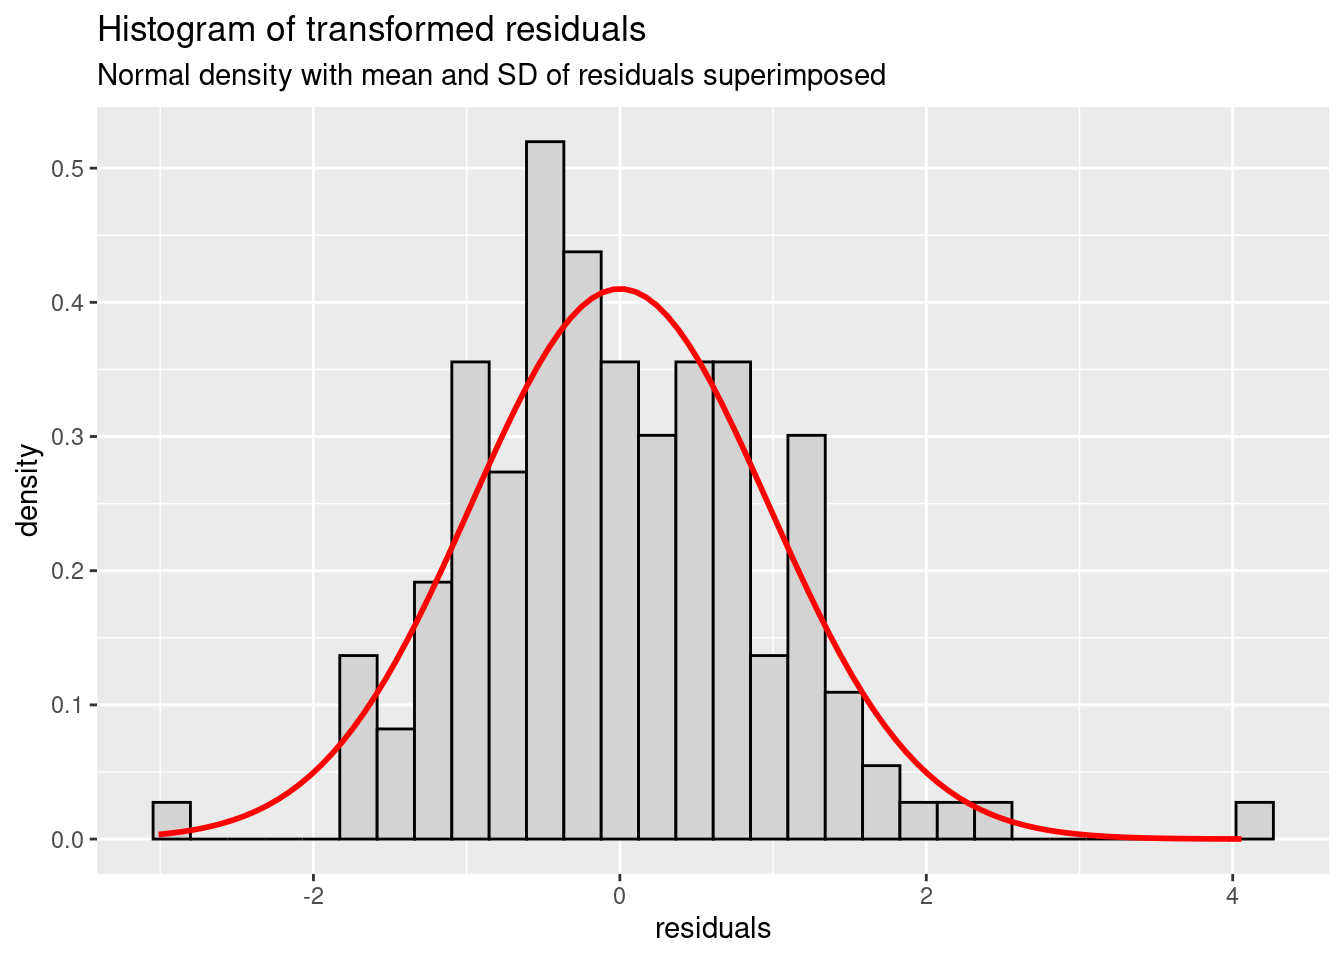
\includegraphics{s2_inference_continuous_files/figure-pdf/unnamed-chunk-22-1.pdf}

}

\end{figure}

Alternatively, we can create a Q-Q-Plot.

\begin{Shaded}
\begin{Highlighting}[]
\NormalTok{df\_residuals }\SpecialCharTok{\%\textgreater{}\%} 
  \FunctionTok{ggplot}\NormalTok{(}\FunctionTok{aes}\NormalTok{(}\AttributeTok{sample =}\NormalTok{ residuals)) }\SpecialCharTok{+}
  \FunctionTok{stat\_qq}\NormalTok{(}\AttributeTok{color =} \StringTok{"blue"}\NormalTok{) }\SpecialCharTok{+}
  \FunctionTok{stat\_qq\_line}\NormalTok{() }\SpecialCharTok{+}
  \FunctionTok{labs}\NormalTok{(}
    \AttributeTok{x =} \StringTok{"Quantiles (Normal distribution)"}\NormalTok{,}
    \AttributeTok{y =} \StringTok{"Transformed Residuals"}
\NormalTok{  ) }\SpecialCharTok{+}
  \FunctionTok{ggtitle}\NormalTok{(}
    \AttributeTok{label =} \StringTok{"Q{-}Q Plot Transformed Residuals Plot"}
\NormalTok{  )}
\end{Highlighting}
\end{Shaded}

\begin{figure}[H]

{\centering 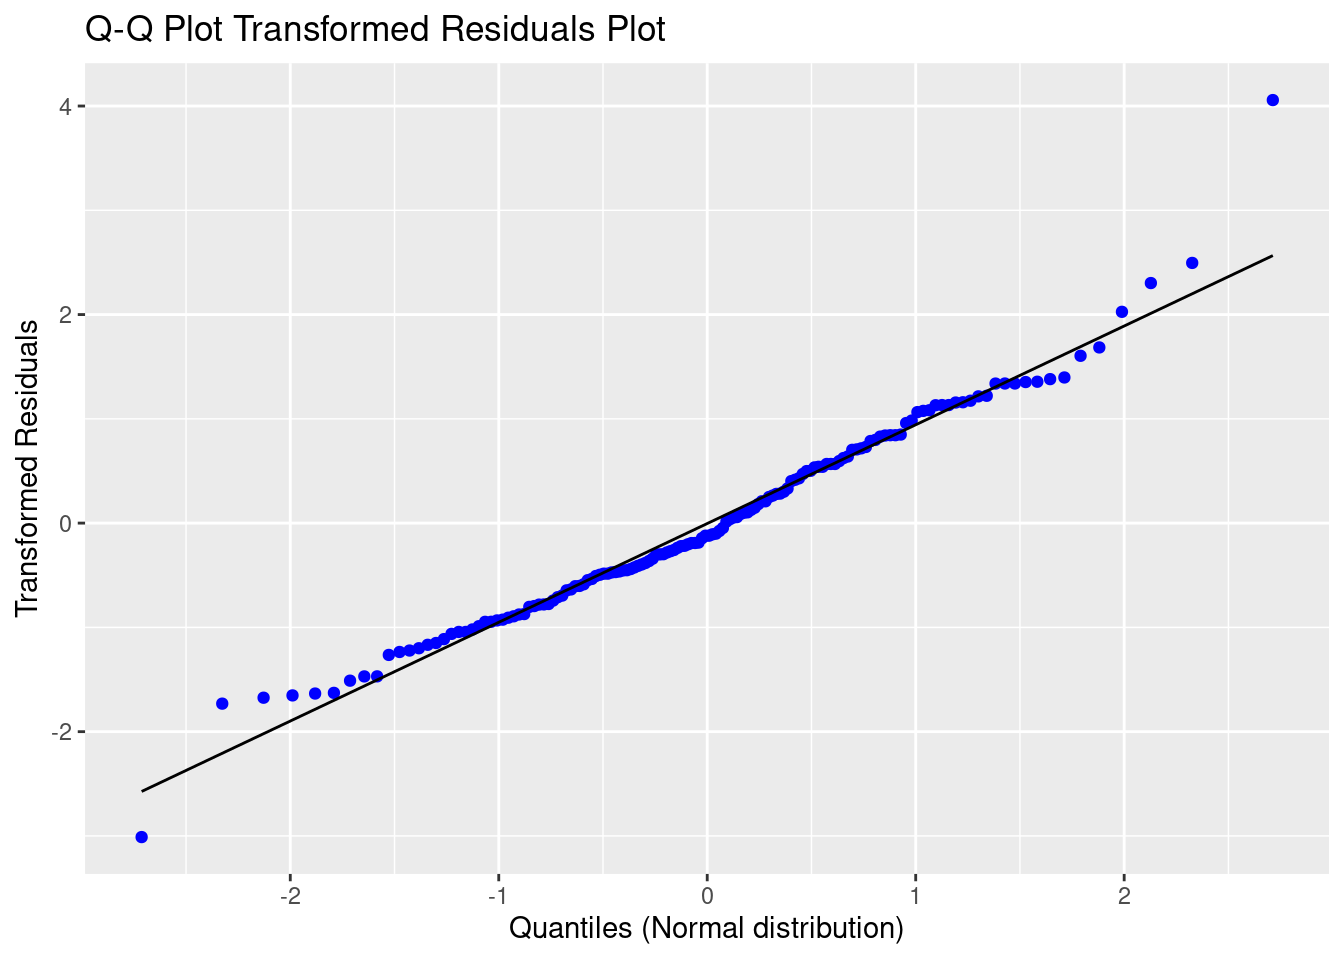
\includegraphics{s2_inference_continuous_files/figure-pdf/unnamed-chunk-23-1.pdf}

}

\end{figure}

How to interprete the Q-Q plot:

We can use the following fourfold table to assess the shape
characteristics derivable from this plot, depending on where the data on
which end of the plot is bend compared to the linear trend line:

\begin{longtable*}{llcc}
\toprule
 &  & \multicolumn{2}{c}{Upper right corner} \\ 
\cmidrule(lr){3-4}
  &   & Above & Below \\ 
\midrule\addlinespace[2.5pt]
Lower left corner & Above & Skewed to the right & Light-tailed \\ 
Lower left corner & Below & Heavy-tailed & Skewed to the left \\ 
\bottomrule
\end{longtable*}

We can see that our data is skewed to the right, as the data in the
upper right corner and data in the lower left corner of the plot bend
above the linear trend line. This is also a trend we can observe from
the histogram.

\begin{Shaded}
\begin{Highlighting}[]
\NormalTok{df\_residuals }\SpecialCharTok{\%\textgreater{}\%} 
  \FunctionTok{ggplot}\NormalTok{(}\FunctionTok{aes}\NormalTok{(}\AttributeTok{x =}\NormalTok{ predictions, }\AttributeTok{y =}\NormalTok{ residuals)) }\SpecialCharTok{+}
  \FunctionTok{geom\_point}\NormalTok{() }\SpecialCharTok{+}
  \FunctionTok{geom\_smooth}\NormalTok{(}\AttributeTok{method =}\NormalTok{ lm, }\AttributeTok{color =} \StringTok{"blue"}\NormalTok{) }\SpecialCharTok{+}
  \FunctionTok{geom\_hline}\NormalTok{(}\AttributeTok{yintercept =} \DecValTok{0}\NormalTok{, }\AttributeTok{show.legend =} \ConstantTok{FALSE}\NormalTok{, }\AttributeTok{linetype =} \DecValTok{2}\NormalTok{) }\SpecialCharTok{+}
  \FunctionTok{ggtitle}\NormalTok{(}
    \AttributeTok{label =} \StringTok{"Residual Plot of predicted values vs. transformed residuals"}
\NormalTok{  )}
\end{Highlighting}
\end{Shaded}

\begin{figure}[H]

{\centering 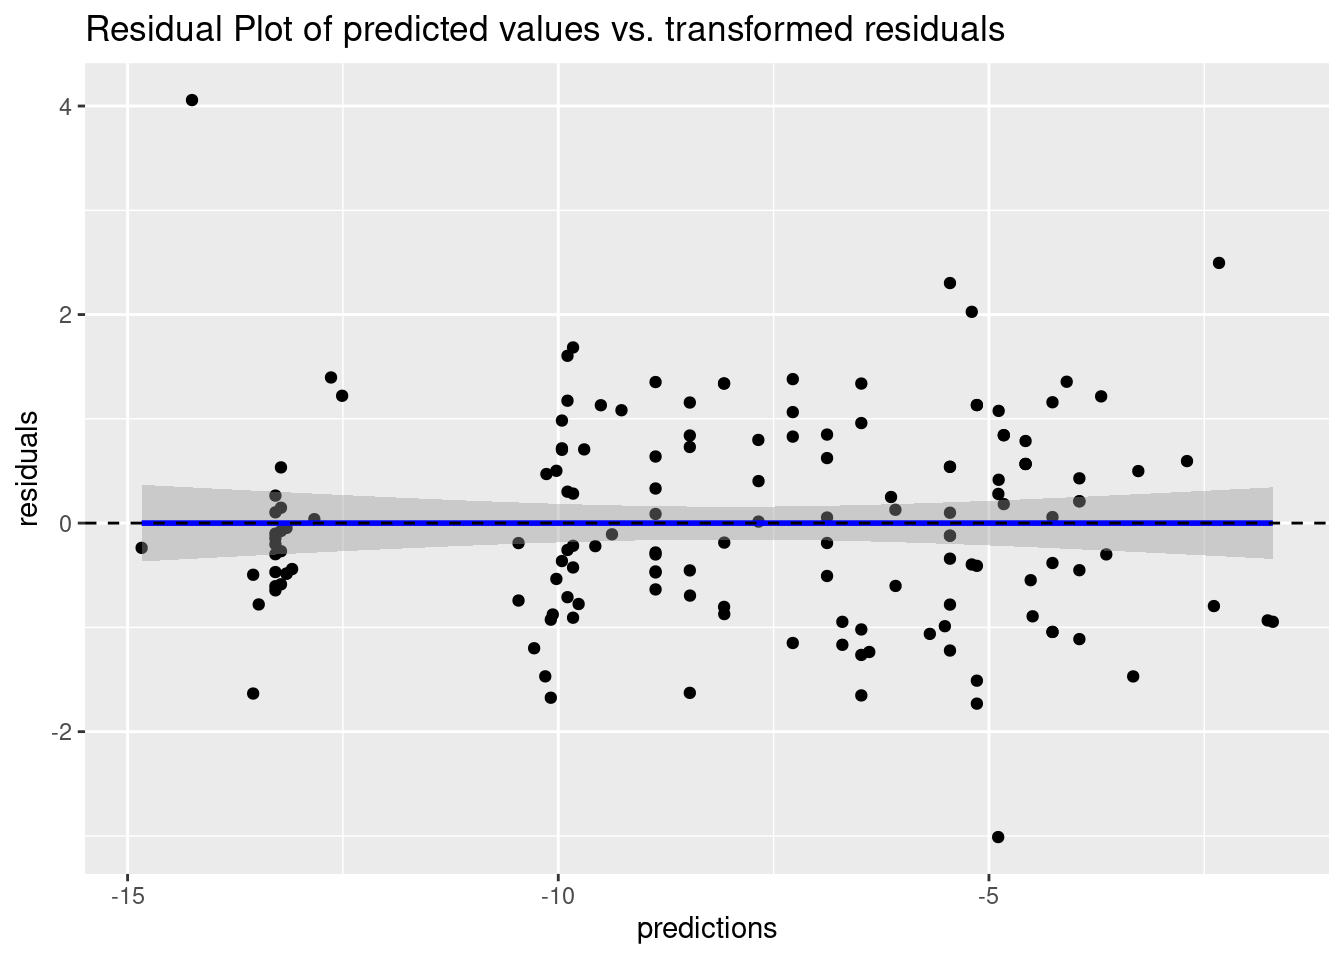
\includegraphics{s2_inference_continuous_files/figure-pdf/unnamed-chunk-25-1.pdf}

}

\end{figure}

What do we see?

\begin{itemize}
\item
  The points in the plot look well dispersed and symmetric around zero.
  The fitted line shows no departure from zero.
\item
  There is no systematic trend, but a rather random scatter.
\item
  We can spot a couple of outliers.
\end{itemize}

\begin{Shaded}
\begin{Highlighting}[]
\NormalTok{df\_residuals }\SpecialCharTok{\%\textgreater{}\%} 
  \FunctionTok{ggplot}\NormalTok{(}\FunctionTok{aes}\NormalTok{(}\AttributeTok{x =}\NormalTok{ predictions, }\AttributeTok{y =}\NormalTok{ change)) }\SpecialCharTok{+}
  \FunctionTok{geom\_point}\NormalTok{() }\SpecialCharTok{+}
  \FunctionTok{geom\_smooth}\NormalTok{(}\AttributeTok{method =}\NormalTok{ lm, }\AttributeTok{color =} \StringTok{"blue"}\NormalTok{)}
\end{Highlighting}
\end{Shaded}

\begin{figure}[H]

{\centering 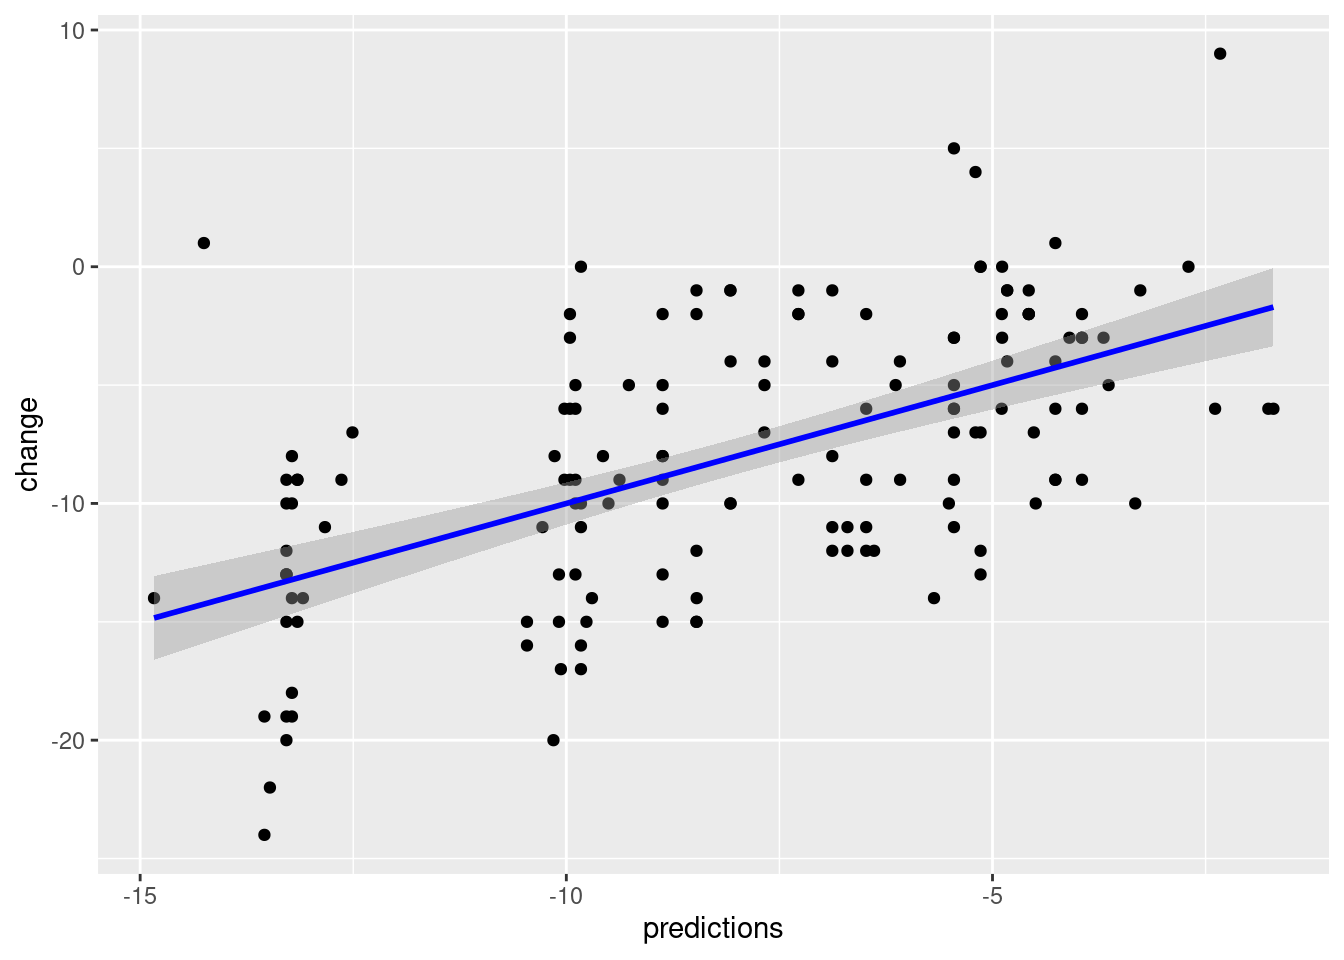
\includegraphics{s2_inference_continuous_files/figure-pdf/unnamed-chunk-26-1.pdf}

}

\end{figure}

\hypertarget{baseline-as-a-response-clda-lda}{%
\section{Baseline as a Response (cLDA +
LDA)}\label{baseline-as-a-response-clda-lda}}

In the former examples we used baseline severity as a continuous
covariate, which is the most common approach. In this case we treat
\texttt{baseval} as a \emph{fixed effect} and used changes from baseline
as response variable in our model formula. This approach comes with a
couple of caveats:

\begin{itemize}
\item
  Only subjects with a non-missing baseline and at least one non-missing
  follow-up response contribute to the analysis (i.e.~at least one
  non-missing change from baseline value).
\item
  Only subjects with complete covariate data contribute to the analysis.
\end{itemize}

Hence, if \texttt{baseval} is missing for a subject, this subject will
not be included in our model. (Liang and Zeger 2000) introduced the
so-called LDA (longitudinal data analysis) and cLDA (constrained
longitudinal data analysis) models. The basic idea behind these models
is that baseline can be regarded as a response at Time 0, and can
therefore be included in the vector of responses.

In order to fit the model, we need to apply some data wrangling upfront
and add baseline to the response column (\texttt{aval}). Note that this
step is usually not required when dealing with CDISC compliant datasets,
such as ADaM or SDTM.

\begin{Shaded}
\begin{Highlighting}[]
\NormalTok{base }\OtherTok{\textless{}{-}}\NormalTok{ dplyr}\SpecialCharTok{::}\FunctionTok{distinct}\NormalTok{(all2, subject, trt, basval, group, gender) }\SpecialCharTok{\%\textgreater{}\%} 
\NormalTok{  dplyr}\SpecialCharTok{::}\FunctionTok{mutate}\NormalTok{(}
    \AttributeTok{time =} \DecValTok{0}\NormalTok{,}
    \AttributeTok{aval =}\NormalTok{ basval,}
    \AttributeTok{avisit =} \StringTok{"Baseline"}
\NormalTok{  )}

\NormalTok{all2\_lda }\OtherTok{\textless{}{-}}\NormalTok{ dplyr}\SpecialCharTok{::}\FunctionTok{bind\_rows}\NormalTok{(all2, base) }\SpecialCharTok{\%\textgreater{}\%} 
\NormalTok{  dplyr}\SpecialCharTok{::}\FunctionTok{mutate}\NormalTok{(}
    \AttributeTok{avisit =}\NormalTok{ forcats}\SpecialCharTok{::}\FunctionTok{fct\_reorder}\NormalTok{(avisit, time)}
\NormalTok{  )}

\DocumentationTok{\#\#\# Check Order of avisit levels:}
\FunctionTok{levels}\NormalTok{(all2\_lda}\SpecialCharTok{$}\NormalTok{avisit)}
\end{Highlighting}
\end{Shaded}

\begin{verbatim}
[1] "Baseline" "Week 2"   "Week 4"   "Week 8"  
\end{verbatim}

We can now fit a model, including \texttt{aval} as a response variable,
treatment (\texttt{group}), visit (\texttt{avisit}) and a
treatment-by-time interaction term:

\begin{Shaded}
\begin{Highlighting}[]
\NormalTok{lda }\OtherTok{\textless{}{-}} \FunctionTok{mmrm}\NormalTok{(}
  \AttributeTok{formula =}\NormalTok{ aval }\SpecialCharTok{\textasciitilde{}}\NormalTok{ group}\SpecialCharTok{*}\NormalTok{avisit }\SpecialCharTok{+} \FunctionTok{us}\NormalTok{(avisit }\SpecialCharTok{|}\NormalTok{ subject),}
  \AttributeTok{data =}\NormalTok{ all2\_lda,}
  \AttributeTok{control =} \FunctionTok{mmrm\_control}\NormalTok{(}\AttributeTok{method =} \StringTok{"Kenward{-}Roger"}\NormalTok{)}
\NormalTok{)}
\end{Highlighting}
\end{Shaded}

The LS Mean estimates per treatment arm for mean changes to Week 8 (Time
3) are now obtained via contrasts between Week 3 and Baseline:

\begin{Shaded}
\begin{Highlighting}[]
\NormalTok{lsmns }\OtherTok{\textless{}{-}} \FunctionTok{emmeans}\NormalTok{(lda, }\SpecialCharTok{\textasciitilde{}}\NormalTok{group}\SpecialCharTok{*}\NormalTok{avisit, }\AttributeTok{weights =} \StringTok{"proportional"}\NormalTok{)}
\FunctionTok{contrast}\NormalTok{(}
\NormalTok{  lsmns,}
  \AttributeTok{method =} \FunctionTok{list}\NormalTok{(}
    \StringTok{"LS Means for Change from Baseline to Week 8 Treatment 1"} \OtherTok{=} \FunctionTok{c}\NormalTok{(}\SpecialCharTok{{-}}\DecValTok{1}\NormalTok{, }\DecValTok{0}\NormalTok{, }\DecValTok{0}\NormalTok{, }\DecValTok{0}\NormalTok{, }\DecValTok{0}\NormalTok{, }\DecValTok{0}\NormalTok{, }\DecValTok{1}\NormalTok{, }\DecValTok{0}\NormalTok{),}
    \StringTok{"LS Means for Change from Baseline to Week 8 Treatment 2"} \OtherTok{=} \FunctionTok{c}\NormalTok{(}\DecValTok{0}\NormalTok{, }\SpecialCharTok{{-}}\DecValTok{1}\NormalTok{, }\DecValTok{0}\NormalTok{, }\DecValTok{0}\NormalTok{, }\DecValTok{0}\NormalTok{, }\DecValTok{0}\NormalTok{, }\DecValTok{0}\NormalTok{, }\DecValTok{1}\NormalTok{),}
    \StringTok{"LS Means for Difference in Changes to Week 8 btw. Treatment 2 and Treatment 1"} \OtherTok{=} \FunctionTok{c}\NormalTok{(}\DecValTok{1}\NormalTok{, }\SpecialCharTok{{-}}\DecValTok{1}\NormalTok{, }\DecValTok{0}\NormalTok{, }\DecValTok{0}\NormalTok{, }\DecValTok{0}\NormalTok{, }\DecValTok{0}\NormalTok{, }\SpecialCharTok{{-}}\DecValTok{1}\NormalTok{, }\DecValTok{1}\NormalTok{)}
\NormalTok{  ), }
  \AttributeTok{adjust =} \ConstantTok{NULL}
\NormalTok{)}
\end{Highlighting}
\end{Shaded}

\begin{verbatim}
 contrast                                                                     
 LS Means for Change from Baseline to Week 8 Treatment 1                      
 LS Means for Change from Baseline to Week 8 Treatment 2                      
 LS Means for Difference in Changes to Week 8 btw. Treatment 2 and Treatment 1
 estimate   SE df t.ratio p.value
    -9.88 1.01 48  -9.768  <.0001
   -13.24 1.01 48 -13.089  <.0001
    -3.36 1.43 48  -2.349  0.0230
\end{verbatim}

A note on caveats associated with LDA models:

\begin{itemize}
\item
  In cases where the treatment effect has a rapid onset, the linearity
  assumption underlying the model is violated.
\item
  Use of baseline as a response, as opposed to a covariate, ignores the
  predictive nature of baseline severity as an explanatory factor in the
  residual error.
\end{itemize}

Generally, LDA models can be very useful in trials with only very few
visits per patient due to the additional response value being included.
In longer trials however, it is recommended to refrain from their use
for the disadvantages stated above. In this case, a decent data quality
should is key to avoid missing baseline data (if possible completely)
and reduce the degree of missingness with regards to follow-up data as
much as possible.

\hypertarget{addendum-on-linear-mixed-effect-models}{%
\section{Addendum on Linear Mixed Effect
Models}\label{addendum-on-linear-mixed-effect-models}}

In this chapter we have dealt with models where the response is modeled
as a linear combination of \emph{fixed effect} parameters \(\beta\) and
a random error \(\varepsilon\)

\[
y = X\beta\,+\,\varepsilon\,.
\]

The fixed effects in this model represent the population effects and we
used the random error to model the subject-specific influences. Although
we used the term mixed model for repeated measures (MMRM), this
nomenclature is misleading in the way that our model does not truly
deserve the term \emph{mixed}. A true mixed model would require the
involvement of \emph{fixed} and \emph{random} effects. The latter have
previously been omitted.

While we will not cover random coefficient models (also known as random
slope and intercept models or RS\&I models) in depth in this class, we
would like to point to couple of useful features. For further reading,
one can refer to Chapter 8 in (Fitzmaurice 2011).

The distinction between \emph{fixed} and \emph{random} effects in linear
mixed effect models allows for modeling of both between-subject and
within-subject variations. In random coefficient models (i.e.~MMRMs with
a non-trivial random effect) each subject is assumed to have their own
(linear) rate of response over time, expressed as random slopes and
intercepts.

``\emph{In addition it is not only possible to estimate parameters that
describe how the mean response changes in the population of interest, it
is also possible to predict how individual response trajectories change
over time. For example, linear mixed effects models can be used to
obtain predictions of individual growth trajectories over time.}''
(Fitzmaurice 2011)

Linear mixed effects models therefore allow for inferences on the
individual (subject) basis rather than the entirety of individuals
(population).

Another advantage of linear mixed models is their flexibility with
respect to imbalances in longitudinal data. We are no longer bound by
the restriction to have (approximately) the same number of observations
per subject, i.e.~the approximately the same length of follow-up, or
even for the visits to be taken at the same times. This feature is
especially useful whenever we are dealing with parallel design studies,
involving the comparison of interventions with different dosing/
assessment frequencies.

Note that the \texttt{mmrm} package so far does not allow for fitting of
linear mixed effect models, in the sense that an actual \emph{random
effects} term is included in the model formula. For these kind of
models, we point to the package \texttt{lme4} (Bates et al. 2015).

\bookmarksetup{startatroot}

\hypertarget{missing-data}{%
\chapter{Missing Data}\label{missing-data}}

So far, we conducted all our analyses on the basis of complete data.
This is a blissful, yet highly unusual setting.

We use the following definition for missing data, borrowed from
(Roderick JA Little 2019):

``\emph{Missing data are unobserved values that would be meaningful for
analysis if observed; in other words, a missing value hides a meaningful
value.}''

We distinguish the following patterns of missingness:

\begin{itemize}
\tightlist
\item
  \textbf{Monotonic missingness/ dropout}: All values by a subject after
  a certain time are missing. More specifically, if responses are
  missing at visit \(n \in \mathbb{N}\), then responses are also missing
  for every subsequent visit \(n + m\), for all \(m \in \mathbb{N}\).
  \emph{Example:} Subject drop-out from the clinical study.
\item
  \textbf{Intermittend missingness}: Subjects miss one or several
  visits, but return for later visits. \emph{Example:} A subject with
  data collected at baseline and Time 1 (Week 2), a missing value at
  Time 2 (Week 4) and a non-missing value at Time 3 (Week 8).
\end{itemize}

Note that, following the nomenclature introduced by (Roderick JA Little
2019), we use the term missing data \emph{pattern}, to describe which
data are missing in the data matrix of subject responses, and the term
missing data \emph{mechanism}, which describes the relationship between
missing and observed values in the subject responses.

Our dataset contains a second variable \texttt{chgdrop}, which is
subject to missingness. Let's rerun our initial MMRM with
\texttt{chgdrop} as dependent variable, baseline value, visit, baseline
by visit interaction and treatment by visit interaction as fixed effects
and an unstructured covariance matrix for visits within each subject.

This formulation is very similar to the one at the beginning of the
former chapter. How do the results differ in terms of LS Means of change
from baseline by treatment arm over time?

\begin{Shaded}
\begin{Highlighting}[]
\NormalTok{fit\_cat\_time }\OtherTok{\textless{}{-}}\NormalTok{ mmrm}\SpecialCharTok{::}\FunctionTok{mmrm}\NormalTok{(}
  \AttributeTok{formula =}\NormalTok{ chgdrop }\SpecialCharTok{\textasciitilde{}}\NormalTok{ basval}\SpecialCharTok{*}\NormalTok{avisit }\SpecialCharTok{+}\NormalTok{ trt}\SpecialCharTok{*}\NormalTok{avisit }\SpecialCharTok{+} \FunctionTok{us}\NormalTok{(avisit }\SpecialCharTok{|}\NormalTok{ subject),}
  \AttributeTok{data =}\NormalTok{ all2,}
  \AttributeTok{control =} \FunctionTok{mmrm\_control}\NormalTok{(}\AttributeTok{method =} \StringTok{"Kenward{-}Roger"}\NormalTok{)}
\NormalTok{)}

\CommentTok{\# summary(fit\_cat\_time)}

\NormalTok{model\_lsmeans }\OtherTok{\textless{}{-}}\NormalTok{ emmeans}\SpecialCharTok{::}\FunctionTok{emmeans}\NormalTok{(fit\_cat\_time, }\SpecialCharTok{\textasciitilde{}}\NormalTok{trt}\SpecialCharTok{*}\NormalTok{avisit, }\AttributeTok{weights =} \StringTok{"proportional"}\NormalTok{)}
\NormalTok{model\_lsmeans}
\end{Highlighting}
\end{Shaded}

\begin{verbatim}
 trt avisit emmean    SE   df lower.CL upper.CL
 1   Week 2  -4.10 0.900 47.0    -5.91    -2.29
 2   Week 2  -5.29 0.899 47.0    -7.10    -3.48
 1   Week 4  -6.42 0.974 46.5    -8.38    -4.46
 2   Week 4  -8.52 0.951 44.8   -10.43    -6.60
 1   Week 8  -9.73 1.142 40.4   -12.03    -7.42
 2   Week 8 -12.62 1.114 40.1   -14.88   -10.37

Confidence level used: 0.95 
\end{verbatim}

\begin{Shaded}
\begin{Highlighting}[]
\NormalTok{emmeans}\SpecialCharTok{::}\FunctionTok{emmeans}\NormalTok{(fit\_cat\_time, }\SpecialCharTok{\textasciitilde{}}\NormalTok{trt}\SpecialCharTok{*}\NormalTok{avisit, }\AttributeTok{weights =} \StringTok{"proportional"}\NormalTok{) }\SpecialCharTok{\%\textgreater{}\%} 
  \FunctionTok{contrast}\NormalTok{(}
    \FunctionTok{list}\NormalTok{(}
      \StringTok{"Difference in LS Means at Week 8"} \OtherTok{=} \FunctionTok{c}\NormalTok{(}\DecValTok{0}\NormalTok{, }\DecValTok{0}\NormalTok{, }\DecValTok{0}\NormalTok{, }\DecValTok{0}\NormalTok{, }\SpecialCharTok{{-}}\DecValTok{1}\NormalTok{, }\DecValTok{1}\NormalTok{),}
      \StringTok{"Difference in longitudinal LS Means to Week 8"} \OtherTok{=} \FunctionTok{c}\NormalTok{(}\SpecialCharTok{{-}}\DecValTok{1}\NormalTok{, }\DecValTok{1}\NormalTok{, }\SpecialCharTok{{-}}\DecValTok{1}\NormalTok{, }\DecValTok{1}\NormalTok{, }\SpecialCharTok{{-}}\DecValTok{1}\NormalTok{, }\DecValTok{1}\NormalTok{)}\SpecialCharTok{/}\DecValTok{3}
\NormalTok{    )}
\NormalTok{  )}
\end{Highlighting}
\end{Shaded}

\begin{verbatim}
 contrast                                      estimate   SE   df t.ratio
 Difference in LS Means at Week 8                 -2.90 1.60 40.3  -1.814
 Difference in longitudinal LS Means to Week 8    -2.06 1.23 46.8  -1.671
 p.value
  0.0772
  0.1014
\end{verbatim}

To understand the nature of the differences between the model using
\texttt{change} as a response variable and the one with
\texttt{chgdrop}, we need to look closer into the extent of missing data
and understand its nature.

\hypertarget{missing-data-mechanisms}{%
\section{Missing Data Mechanisms}\label{missing-data-mechanisms}}

To understand the nature of missing data in our clinical trial, we
consider the following taxonomy, introduced by (Roderick JA Little
2019). We differentiate between the following three types of missing
data:

\begin{itemize}
\item
  \textbf{Missing Completely at Random (MCAR)}: Conditional on all
  covariates in our analysis, the probability of missingness does not
  depend on either observed or unobserved values of the response
  variable.
\item
  \textbf{Missing at Random (MAR)}: Conditional on all covariates and
  observed response values in our analysis, the probability of
  missingness does not depend on the unobserved values of the response
  variable.
\item
  \textbf{Missing not at Random (MNAR)}: Conditional on all covariates
  and observed response values in our analysis, the probability of
  missingness does depend on the unobserved values of the response
  variable.
\end{itemize}

(Mallinckrodt and Lipkovich 2016) give the following interpretation
around the three types of missingness:

``\emph{With MCAR, the outcome variable is not related to the
probability of dropout (after taking into account covariates). In MAR,
the observed values of the outcome variable are related to the
probability of dropout, but the unobserved outcomes are not (after
taking into account covariates and observed outcomes). In MNAR the
unobserved outcomes are related to the probability of dropout even after
the observed outcomes and covariates have been taken into account.}''

The following two sections outline handling strategies for missing data.
However, the best approach to handle missing data is to minimise its
extent. While the occurence of missing data can rarely be avoided at all
(think about the collection of questionnaire data in oncology studies
and the missing data after subjects die), it is important to pursue an
``as complete as can be'' data collection.

Baseline and screening data are of utmost importance in a pursuit of
data completeness. If a screening value is missing, but was meant to be
used as a covariate, this subjects' whole data will be dropped from the
analysis even if all responses were observed. If the baseline response
variable was missing we are unable to compute a change from baseline,
which also leads to the loss of this subjects' data in the model
(although LDA models are still able to provide an estimate) even if all
post-baseline values were observed.

\hypertarget{missing-data-handling-i-descriptive-stats-visualisations}{%
\section{Missing data handling I (descriptive stats +
visualisations)}\label{missing-data-handling-i-descriptive-stats-visualisations}}

To gain an understanding of the impact of missingness on the average
response trajectories, we can plot the mean changes from baseline by
visit for each drop-out group. The three drop-out groups (variable
\texttt{dropout\_grp}) are:

\begin{itemize}
\item
  Drop-outs at Week 2: Subjects who completed baseline and Week 2, but
  discontinued from the study prior to Week 4.
\item
  Drop-outs at Week 4: Subjects who completed baseline, Week 2 and Week
  4, but discontinued from the study prior to Week 8.
\item
  Completers: Subjects who completed all visits in the study.
\end{itemize}

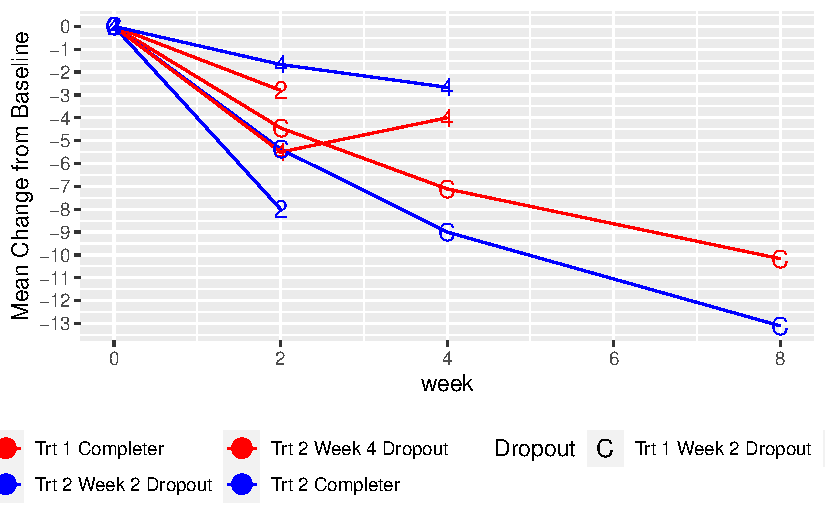
\includegraphics{s3_missingness_files/figure-pdf/unnamed-chunk-3-1.pdf}

\textbf{Exercise:} Try to interpret the plot above and discuss the
following topics around missingness:

\begin{itemize}
\item
  Look into the data. Which missing data pattern is present in this
  dataset?
\item
  What can be seen in the plot? How does the drop-out time affect the
  observed mean response trajectories?
\item
  What other aspects, apart from response, could influence a subjects'
  likelihood to drop-out from the study?
\item
  Which other summaries/ visualizations can be useful to characterize
  and monitor the degree of missingness in clinical study data?
\end{itemize}

\textbf{Solution:} A look into the data shows that all missing values
stem from a monotinic missingness pattern.

The figure above shows a notable difference between mean response
trajectories per drop-out group. The completers in both treatment arms
show a steady decrease of HAMD17 scores over time, which is equivalent
to an increase in depression symptoms.

Week 4 drop-outs under treatment 2 only showed a moderate change from
baseline, while the treatment 1 subjects experienced an increase in
HAMD17 scores. A possible explanation could be that changes under
treatment 2 were not regarded meaningful by patients, while the increase
in scores under treatment 1 made subjects drop out of the study.

Week 2 drop-outs under treatment 2 showed notable improvements of HAMD17
scores compared to treatment 1, yet the drop-out could potentially be
linked to the occurrence of adverse events.

Although the extent of missing data should be reduced to the bare
minimum, it can never be avoided completely, especially with
Patient-Reported Outcomes (PRO) data. In the reporting of PRO clinical
trial data, it is therefore important to transparently summarize the
extent of missingness. This is usually done via so-called
\emph{compliance tables}.

Compliance tables summarize three key components to characterize
missingness in our data:

\begin{itemize}
\item
  The number of subjects initially randomized in the trial.
\item
  The number of subjects for whom data is expected. This is the number
  of patients who are still ongoing in the study (alive and not
  discontinued) and for whom an assessment is scheduled following the
  schedule of assessments in the clinical trial protocol.
\item
  The number of subjects by whom the assessment has been completed.
\end{itemize}

From these numbers, we can derive the \emph{available data rate} and the
\emph{compliance} for visit \(i\) as follows:

\[
\begin{align}
\text{Available Data Rate}_{\,i} &:= 100\,\frac{\#\{\text{Subj. with assessment i completed}\}}{\#\{\text{Subj. randomized}\}}\,,\\
\text{Compliance Rate}_{\,i} &:= 100\,\frac{\#\{\text{Subj. with assessment i completed}\}}{\#\{\text{Subj. assessment i expected}\}}\,.
\end{align}
\] The available data rate indicates the degree of missingness due to
drop-outs or deaths from the study. It shows how many of the initially
randomized patients are still ongoing at a certain visit.

The compliance rate indicates the degree of missingness due to skipped
assessments by patients, who are still ongoing in the study and expected
to provide their measurement.

One can summarize compliance and available data rate by means of a table
or stacked bar charts with study visits on the x-axis and percentage of
patients with measurements at the respective visit, drop-out, skipped
assessments, death etc. on the y-axis.

\hypertarget{missing-data-handling-ii-naive-analytic-approaches}{%
\section{Missing data handling II (naive analytic
approaches)}\label{missing-data-handling-ii-naive-analytic-approaches}}

This section provides an overview of simple and most of the times overly
naive methods to deal with missing data. Although we will introduce more
suitable methods in the next chapter, the approaches introduced in this
section have gained questionable popularity in the past, which is why we
introduce them here. The following methods to compute or completely
ignore missing data exist:

\begin{itemize}
\item
  Complete Case Analysis: Discard all subjects with missing observations
  and only conduct the analysis on subjects with complete follow-up
  data.
\item
  Last observation carried forward (LOCF): Handling of monotonic missing
  data. The missing visits are imputed with the last non-missing value.
  This approach assumes a constant trend of observations after drop-out
  from the study, i.e.~the response level remains the same as the last
  response under the study drug.
\item
  Baseline observation carried forward (BOCF): Handling of monotonic
  missing data. The missing visits are imputed with the baseline value.
  This approach assumes that subjects' symptom severity or functioning
  (whichever was measured in the study) \emph{bounce back} to the
  baseline state, prior to the intiation of the study drug.
\end{itemize}

\hypertarget{complete-case-analyses}{%
\subsection{Complete Case Analyses}\label{complete-case-analyses}}

Let us run a complete case analysis on the \texttt{all2} dataset.

\textbf{Exercise:} Fit an MMRM with response variable \texttt{chgdrop},
with baseline severity, treatment and visit as fixed effects, as well as
baseline-by-visit and treatment-by-visit interaction, using an
unstructured variance-covariance matrix on the \texttt{all2} completers.

\begin{itemize}
\item
  How do the results differ from the results obtained in the former
  chapter (response variable \texttt{change}, no missing data)?
\item
  How do the results differ from the results obtained at the beginning
  of this chapter (response variable \texttt{chgdrop} with missing
  data)?
\item
  Discuss the limitations of the complete case analysis. Which sources
  of bias can you identify?
\end{itemize}

\textbf{Solution:}

We firstly select our completers dataset. As this is a filtering
exercise based on post-baseline characteristics, we first look into the
distribution of subjects per treatment arm (note that we lost our
randomization effect):

\begin{Shaded}
\begin{Highlighting}[]
\DocumentationTok{\#\#\# Completers only}
\NormalTok{all2\_comp }\OtherTok{\textless{}{-}}\NormalTok{ dplyr}\SpecialCharTok{::}\FunctionTok{filter}\NormalTok{(all2, dropout\_grp }\SpecialCharTok{==} \StringTok{"Completer"}\NormalTok{)}

\NormalTok{all2\_comp }\SpecialCharTok{\%\textgreater{}\%} 
\NormalTok{  dplyr}\SpecialCharTok{::}\FunctionTok{group\_by}\NormalTok{(group) }\SpecialCharTok{\%\textgreater{}\%} 
\NormalTok{  dplyr}\SpecialCharTok{::}\FunctionTok{summarise}\NormalTok{(}
    \AttributeTok{N =}\NormalTok{ dplyr}\SpecialCharTok{::}\FunctionTok{n\_distinct}\NormalTok{(subject),}
    \AttributeTok{.groups =} \StringTok{"drop"}
\NormalTok{  )}
\end{Highlighting}
\end{Shaded}

\begin{verbatim}
# A tibble: 2 x 2
  group     N
  <fct> <int>
1 Arm 1    18
2 Arm 2    19
\end{verbatim}

In this case, we are left with 18 and 19 subjects per arm, which reduced
our sample size notably, but at least left us with close to equal sizes
of our treatment groups. This is not normal. Usually the stratification
of data based on post-baseline assessments can lead to imbalances (it
might still have, as we only checked the distribution of the treatment
arms).

\begin{Shaded}
\begin{Highlighting}[]
\DocumentationTok{\#\#\# Complete Case Analysis}
\NormalTok{fit\_cat\_time\_compl }\OtherTok{\textless{}{-}}\NormalTok{ mmrm}\SpecialCharTok{::}\FunctionTok{mmrm}\NormalTok{(}
  \AttributeTok{formula =}\NormalTok{ chgdrop }\SpecialCharTok{\textasciitilde{}}\NormalTok{ basval}\SpecialCharTok{*}\NormalTok{avisit }\SpecialCharTok{+}\NormalTok{ trt}\SpecialCharTok{*}\NormalTok{avisit }\SpecialCharTok{+} \FunctionTok{us}\NormalTok{(avisit }\SpecialCharTok{|}\NormalTok{ subject),}
  \AttributeTok{data =}\NormalTok{ all2\_comp,}
  \AttributeTok{control =} \FunctionTok{mmrm\_control}\NormalTok{(}\AttributeTok{method =} \StringTok{"Kenward{-}Roger"}\NormalTok{)}
\NormalTok{)}

\FunctionTok{summary}\NormalTok{(fit\_cat\_time\_compl)}
\end{Highlighting}
\end{Shaded}

\begin{verbatim}
mmrm fit

Formula:     chgdrop ~ basval * avisit + trt * avisit + us(avisit | subject)
Data:        all2_comp (used 111 observations from 37 subjects with maximum 3 
timepoints)
Covariance:  unstructured (6 variance parameters)
Method:      Kenward-Roger
Vcov Method: Kenward-Roger
Inference:   REML

Model selection criteria:
     AIC      BIC   logLik deviance 
   608.8    618.5   -298.4    596.8 

Coefficients: 
                     Estimate Std. Error        df t value Pr(>|t|)    
(Intercept)           1.89223    3.60558  33.99000   0.525 0.603124    
basval               -0.31950    0.17281  33.99000  -1.849 0.073201 .  
avisitWeek 4         -1.63943    2.46046  34.00000  -0.666 0.509708    
avisitWeek 8        -12.36928    3.39084  34.00000  -3.648 0.000877 ***
trt2                 -1.13978    1.56623  33.99000  -0.728 0.471768    
basval:avisitWeek 4  -0.05179    0.11793  34.00000  -0.439 0.663301    
basval:avisitWeek 8   0.33515    0.16252  34.00000   2.062 0.046899 *  
avisitWeek 4:trt2    -0.99990    1.06880  34.00000  -0.936 0.356113    
avisitWeek 8:trt2    -1.78825    1.47295  34.00000  -1.214 0.233089    
---
Signif. codes:  0 '***' 0.001 '**' 0.01 '*' 0.05 '.' 0.1 ' ' 1

Covariance estimate:
        Week 2  Week 4  Week 8
Week 2 23.2319 16.8721 14.6422
Week 4 16.8721 21.7589 17.9166
Week 8 14.6422 17.9166 27.5347
\end{verbatim}

\begin{Shaded}
\begin{Highlighting}[]
\NormalTok{model\_lsmeans }\OtherTok{\textless{}{-}}\NormalTok{ emmeans}\SpecialCharTok{::}\FunctionTok{emmeans}\NormalTok{(fit\_cat\_time\_compl, }\SpecialCharTok{\textasciitilde{}}\NormalTok{trt}\SpecialCharTok{*}\NormalTok{avisit, }\AttributeTok{weights =} \StringTok{"proportional"}\NormalTok{)}
\NormalTok{model\_lsmeans}
\end{Highlighting}
\end{Shaded}

\begin{verbatim}
 trt avisit emmean   SE df lower.CL upper.CL
 1   Week 2  -4.33 1.12 34    -6.61    -2.06
 2   Week 2  -5.47 1.09 34    -7.69    -3.26
 1   Week 4  -6.98 1.09 34    -9.19    -4.77
 2   Week 4  -9.12 1.06 34   -11.27    -6.97
 1   Week 8 -10.17 1.21 34   -12.63    -7.71
 2   Week 8 -13.10 1.18 34   -15.49   -10.71

Confidence level used: 0.95 
\end{verbatim}

\begin{Shaded}
\begin{Highlighting}[]
\NormalTok{emmeans}\SpecialCharTok{::}\FunctionTok{emmeans}\NormalTok{(fit\_cat\_time\_compl, }\SpecialCharTok{\textasciitilde{}}\NormalTok{trt}\SpecialCharTok{*}\NormalTok{avisit, }\AttributeTok{weights =} \StringTok{"proportional"}\NormalTok{) }\SpecialCharTok{\%\textgreater{}\%} 
  \FunctionTok{contrast}\NormalTok{(}
    \FunctionTok{list}\NormalTok{(}
      \StringTok{"Difference in LS Means at Week 8"} \OtherTok{=} \FunctionTok{c}\NormalTok{(}\DecValTok{0}\NormalTok{, }\DecValTok{0}\NormalTok{, }\DecValTok{0}\NormalTok{, }\DecValTok{0}\NormalTok{, }\SpecialCharTok{{-}}\DecValTok{1}\NormalTok{, }\DecValTok{1}\NormalTok{),}
      \StringTok{"Difference in longitudinal LS Means to Week 8"} \OtherTok{=} \FunctionTok{c}\NormalTok{(}\SpecialCharTok{{-}}\DecValTok{1}\NormalTok{, }\DecValTok{1}\NormalTok{, }\SpecialCharTok{{-}}\DecValTok{1}\NormalTok{, }\DecValTok{1}\NormalTok{, }\SpecialCharTok{{-}}\DecValTok{1}\NormalTok{, }\DecValTok{1}\NormalTok{)}\SpecialCharTok{/}\DecValTok{3}
\NormalTok{    )}
\NormalTok{  )}
\end{Highlighting}
\end{Shaded}

\begin{verbatim}
 contrast                                      estimate   SE df t.ratio p.value
 Difference in LS Means at Week 8                 -2.93 1.69 34  -1.733  0.0922
 Difference in longitudinal LS Means to Week 8    -2.07 1.42 34  -1.455  0.1548
\end{verbatim}

A comparison to the results using the full response trajectories for all
randomized subjects (response variable \texttt{change}) yields:

\begin{Shaded}
\begin{Highlighting}[]
\DocumentationTok{\#\#\# complete response trajectory on all randomized subjects}

\NormalTok{fit\_cat\_time }\OtherTok{\textless{}{-}}\NormalTok{ mmrm}\SpecialCharTok{::}\FunctionTok{mmrm}\NormalTok{(}
  \AttributeTok{formula =}\NormalTok{ change }\SpecialCharTok{\textasciitilde{}}\NormalTok{ basval}\SpecialCharTok{*}\NormalTok{avisit }\SpecialCharTok{+}\NormalTok{ trt}\SpecialCharTok{*}\NormalTok{avisit }\SpecialCharTok{+} \FunctionTok{us}\NormalTok{(avisit }\SpecialCharTok{|}\NormalTok{ subject),}
  \AttributeTok{data =}\NormalTok{ all2,}
  \AttributeTok{control =} \FunctionTok{mmrm\_control}\NormalTok{(}\AttributeTok{method =} \StringTok{"Kenward{-}Roger"}\NormalTok{)}
\NormalTok{)}

\NormalTok{model\_lsmeans }\OtherTok{\textless{}{-}}\NormalTok{ emmeans}\SpecialCharTok{::}\FunctionTok{emmeans}\NormalTok{(fit\_cat\_time, }\SpecialCharTok{\textasciitilde{}}\NormalTok{trt}\SpecialCharTok{*}\NormalTok{avisit, }\AttributeTok{weights =} \StringTok{"proportional"}\NormalTok{)}
\NormalTok{model\_lsmeans}
\end{Highlighting}
\end{Shaded}

\begin{verbatim}
 trt avisit emmean    SE df lower.CL upper.CL
 1   Week 2  -4.13 0.899 47    -5.93    -2.32
 2   Week 2  -5.31 0.899 47    -7.12    -3.51
 1   Week 4  -6.70 0.916 47    -8.55    -4.86
 2   Week 4  -8.70 0.916 47   -10.54    -6.85
 1   Week 8  -9.86 1.033 47   -11.94    -7.79
 2   Week 8 -13.26 1.033 47   -15.33   -11.18

Confidence level used: 0.95 
\end{verbatim}

\begin{Shaded}
\begin{Highlighting}[]
\NormalTok{emmeans}\SpecialCharTok{::}\FunctionTok{emmeans}\NormalTok{(fit\_cat\_time, }\SpecialCharTok{\textasciitilde{}}\NormalTok{trt}\SpecialCharTok{*}\NormalTok{avisit, }\AttributeTok{weights =} \StringTok{"proportional"}\NormalTok{) }\SpecialCharTok{\%\textgreater{}\%} 
  \FunctionTok{contrast}\NormalTok{(}
    \FunctionTok{list}\NormalTok{(}
      \StringTok{"Difference in LS Means at Week 8"} \OtherTok{=} \FunctionTok{c}\NormalTok{(}\DecValTok{0}\NormalTok{, }\DecValTok{0}\NormalTok{, }\DecValTok{0}\NormalTok{, }\DecValTok{0}\NormalTok{, }\SpecialCharTok{{-}}\DecValTok{1}\NormalTok{, }\DecValTok{1}\NormalTok{),}
      \StringTok{"Difference in longitudinal LS Means to Week 8"} \OtherTok{=} \FunctionTok{c}\NormalTok{(}\SpecialCharTok{{-}}\DecValTok{1}\NormalTok{, }\DecValTok{1}\NormalTok{, }\SpecialCharTok{{-}}\DecValTok{1}\NormalTok{, }\DecValTok{1}\NormalTok{, }\SpecialCharTok{{-}}\DecValTok{1}\NormalTok{, }\DecValTok{1}\NormalTok{)}\SpecialCharTok{/}\DecValTok{3}
\NormalTok{    )}
\NormalTok{  )}
\end{Highlighting}
\end{Shaded}

\begin{verbatim}
 contrast                                      estimate   SE df t.ratio p.value
 Difference in LS Means at Week 8                 -3.39 1.46 47  -2.319  0.0248
 Difference in longitudinal LS Means to Week 8    -2.19 1.18 47  -1.850  0.0705
\end{verbatim}

We can see that the mean change from baseline to Week 8 using the
complete response trajectory is actually lower (i.e.~better) under
Treatment 2 than the ones from the complete case analysis. For Treatment
1 the mean change from baseline to Week 8 is a little higher
(i.e.~worse) for the complete response trajectory on all randomized
subjects as compared to the complete case analysis. A possible
explanation could be that the favorable treatment effect of Treatment 2
came at the cost of adverse events, which made subjects drop out from
the study, while the lack of early efficacy under Treatment 1 made
subjects drop out, which lead them to not experience the favorable
effects in the longer term.

A comparison to the analysis results based on the incomplete response
trajectory (data as is), yields:

\begin{Shaded}
\begin{Highlighting}[]
\DocumentationTok{\#\#\# Response data as is (including missings)}

\NormalTok{fit\_cat\_time }\OtherTok{\textless{}{-}}\NormalTok{ mmrm}\SpecialCharTok{::}\FunctionTok{mmrm}\NormalTok{(}
  \AttributeTok{formula =}\NormalTok{ chgdrop }\SpecialCharTok{\textasciitilde{}}\NormalTok{ basval}\SpecialCharTok{*}\NormalTok{avisit }\SpecialCharTok{+}\NormalTok{ trt}\SpecialCharTok{*}\NormalTok{avisit }\SpecialCharTok{+} \FunctionTok{us}\NormalTok{(avisit }\SpecialCharTok{|}\NormalTok{ subject),}
  \AttributeTok{data =}\NormalTok{ all2,}
  \AttributeTok{control =} \FunctionTok{mmrm\_control}\NormalTok{(}\AttributeTok{method =} \StringTok{"Kenward{-}Roger"}\NormalTok{)}
\NormalTok{)}

\NormalTok{emmeans}\SpecialCharTok{::}\FunctionTok{emmeans}\NormalTok{(fit\_cat\_time, }\SpecialCharTok{\textasciitilde{}}\NormalTok{trt}\SpecialCharTok{*}\NormalTok{avisit, }\AttributeTok{weights =} \StringTok{"proportional"}\NormalTok{)}
\end{Highlighting}
\end{Shaded}

\begin{verbatim}
 trt avisit emmean    SE   df lower.CL upper.CL
 1   Week 2  -4.10 0.900 47.0    -5.91    -2.29
 2   Week 2  -5.29 0.899 47.0    -7.10    -3.48
 1   Week 4  -6.42 0.974 46.5    -8.38    -4.46
 2   Week 4  -8.52 0.951 44.8   -10.43    -6.60
 1   Week 8  -9.73 1.142 40.4   -12.03    -7.42
 2   Week 8 -12.62 1.114 40.1   -14.88   -10.37

Confidence level used: 0.95 
\end{verbatim}

\begin{Shaded}
\begin{Highlighting}[]
\NormalTok{emmeans}\SpecialCharTok{::}\FunctionTok{emmeans}\NormalTok{(fit\_cat\_time, }\SpecialCharTok{\textasciitilde{}}\NormalTok{trt}\SpecialCharTok{*}\NormalTok{avisit, }\AttributeTok{weights =} \StringTok{"proportional"}\NormalTok{) }\SpecialCharTok{\%\textgreater{}\%} 
  \FunctionTok{contrast}\NormalTok{(}
    \FunctionTok{list}\NormalTok{(}
      \StringTok{"Difference in LS Means at Week 8"} \OtherTok{=} \FunctionTok{c}\NormalTok{(}\DecValTok{0}\NormalTok{, }\DecValTok{0}\NormalTok{, }\DecValTok{0}\NormalTok{, }\DecValTok{0}\NormalTok{, }\SpecialCharTok{{-}}\DecValTok{1}\NormalTok{, }\DecValTok{1}\NormalTok{),}
      \StringTok{"Difference in longitudinal LS Means to Week 8"} \OtherTok{=} \FunctionTok{c}\NormalTok{(}\SpecialCharTok{{-}}\DecValTok{1}\NormalTok{, }\DecValTok{1}\NormalTok{, }\SpecialCharTok{{-}}\DecValTok{1}\NormalTok{, }\DecValTok{1}\NormalTok{, }\SpecialCharTok{{-}}\DecValTok{1}\NormalTok{, }\DecValTok{1}\NormalTok{)}\SpecialCharTok{/}\DecValTok{3}
\NormalTok{    )}
\NormalTok{  )}
\end{Highlighting}
\end{Shaded}

\begin{verbatim}
 contrast                                      estimate   SE   df t.ratio
 Difference in LS Means at Week 8                 -2.90 1.60 40.3  -1.814
 Difference in longitudinal LS Means to Week 8    -2.06 1.23 46.8  -1.671
 p.value
  0.0772
  0.1014
\end{verbatim}

We can see that mean changes from baseline to Week 8 are higher
(i.e.~worse) under both treatment arms using the data as is, as compared
to the complete case analysis. In this case, the complete case analysis
overestimates the treatment effect in both arms. This effect is often
observed with complete case analyses, due to the inherent selection bias
that arises from the inclusion of completers only.

\hypertarget{discussion}{%
\subsection{Discussion}\label{discussion}}

Complete Case Analysis is subject to selection bias, as the analysis is
only conducted on subjects who complete the study and therefore did not
drop out due to the experience of adverse events of the lack of
efficacy. Selection of subjects based on post-baseline events can lead
to notable imbalances between our treatment arms and the distribution of
covariates. Results from the Complete Case Analysis can therefore be
hard to interpret (due to the loss of randomization), and are frequently
overestimating the true treatment effect.

In principle, this method should be avoided.

\bookmarksetup{startatroot}

\hypertarget{sensitivity-analyses}{%
\chapter{Sensitivity Analyses}\label{sensitivity-analyses}}

Purpose: talk about sensitivity analyses with respect to missing data

\begin{itemize}
\tightlist
\item
  MMRM is an appropriate choice for the primary analysis in many
  longitudinal clinical trials under the missing at random (MAR)
  assumption.
\item
  MMRM can handle missing values. BUT: need of baseline and at least one
  post-baseline value.
\item
  No imputation for individual missing values but missing data is
  implicitly imputed.
\item
  Exploit the correlation between outcomes within subjects.
\item
  MAR: future outcomes for subjects who discontinued are assumed be
  similar to the future outcomes of subjects who continued if they had
  the same values of past (observed) outcomes, covariates,\ldots{}
\end{itemize}

\hypertarget{purpose-of-sensitivity-analyses}{%
\section{Purpose of sensitivity
analyses}\label{purpose-of-sensitivity-analyses}}

\begin{itemize}
\tightlist
\item
  Consider sensivitiy analyses to check model assumptions
  e.g.~assumption of MAR.
\item
  Comparing results from sensitivity analyses: how much inference rely
  on the assumptions.
\item
  Here, inference with regard to the treatment effect. Thus, investigate
  how treatment effects vary depending on assumptions (about missing
  data).
\item
  Uncertainty from incompleteness cannot be objectively evaluated from
  observed data so there is a need for missing data sensitivity
  analyses.
\end{itemize}

\hypertarget{mmrm-vs.-mi}{%
\section{MMRM vs.~MI}\label{mmrm-vs.-mi}}

\begin{itemize}
\tightlist
\item
  Flexibility in modeling treatment effects over time and the
  within-patient error correlation structure makes MMRM a widely useful
  analysis.
\item
  MMRM, MI: two major approaches to missing data with good statistical
  properties. Both rely on MAR assumption (for MI: standard
  implementation).
\item
  MMRM: missing values implicitly imputed, MI: missing values explicitly
  imputed.
\item
  MMRM vs.~MI: approximately equivalent provided the variables used in
  the imputation model are the same as those included in the analysis
  model (level of equivalence will depend on the number of imputations)
\item
  MI: imputation model with at least those variables from the primary
  model, additional auxiliary variables can be used in the imputation
  model to improve the accuracy of the missing data prediction.
\item
  Handling missing not at random (MNAR) possible for MI
  (e.g.~reference-based imputation) but not within MMRM.
\item
  MMRM does not work if missing baseline values are present. Missing
  baseline values can be imputed first. Additionally, at least one
  post-baseline value has to be observed. Alternative: LDA where
  baseline is part of the response vector.
\end{itemize}

Note that, when implemented in similar manners, MI and MMRM have similar
assumptions and yield similar results. Thus, MI implemented similarly to
MMRM is not a sensitivity analysis!

\hypertarget{missing-covariates-baseline-data-only}{%
\section{Missing covariates (baseline data)
only}\label{missing-covariates-baseline-data-only}}

\begin{itemize}
\tightlist
\item
  Missing baseline value of the outcome (and other covariates) is a
  common situation
\item
  MMRM not efficient or potential biased estimates as subjects with
  missing covariates are excluded from the analysis
\item
  (Kayembe and Breukelen 2022) compared different methods
  e.g.~unadjusted analysis, complete case, mean imputation, MI: mean
  imputation seems to be appropriate as long as the covariates are
  measured before randomization (produces unbiased treatment effect
  estimates with good coverage, easy to implement)
\end{itemize}

Now, we consider the situation as in our data sets: baseline observed,
no intermittent missing values, drop-outs = monotone missing pattern

\hypertarget{sensitivity-analyses---simple-approaches}{%
\section{Sensitivity analyses - Simple
approaches}\label{sensitivity-analyses---simple-approaches}}

In general, these simple approaches are not recommended for use. Methods
are of historic interest and provide a useful starting point. Here, we
consider two simple approaches. We will apply these two methods in the
practical part to compare results.

\hypertarget{last-observation-carried-forward-locf}{%
\subsection{Last observation carried forward
(LOCF)}\label{last-observation-carried-forward-locf}}

LOCF imputes all missing values for each subject using the last observed
value for that subject. Typically, under LOCF the repeated masures
nature of the data is ignored and a single outcome for each subject is
analyzed. LOCF was used in the past, justified as it was thought that it
provides conservative estimates. However, conditions under which LOCF
yield conservative estimates and maintain control of Type I error rates
are not straightforward and cannot be assured at the beginning of the
trial. For example, LOCF is likely to overestimate treatment benefit if
dop-out in the control gorup is more frequent.

\hypertarget{complete-case-cc}{%
\subsection{Complete case (CC)}\label{complete-case-cc}}

Other names: observed case/ completers analysis

Reduce the data set selecting only those subjects with observed outcome
value(s).

Completers analysis may create selection bias, may cause overestimation
of within group effects particularly at the last scheduled visit.

\hypertarget{sensitivity-analyses---handling-nonignorable-missingness-mnar}{%
\section{Sensitivity analyses - Handling nonignorable missingness
(MNAR)}\label{sensitivity-analyses---handling-nonignorable-missingness-mnar}}

\begin{itemize}
\tightlist
\item
  Assumption of MAR is often reasonable, but possibility of data missing
  not at random (MNAR) is difficult to rule out.
\item
  Thus, analysis under MNAR needed.
\item
  Analysis under MNAR: these methods are heavily assumption driven and
  the assumptions are not testable as we do not have the missing data.
\item
  Consider a sensitivity analysis framework allowing assessment of
  robustness of results to the various assumptions.
\item
  MNAR methods: different possibilities e.g.~class of pattern-mixture
  models. The pattern-mixture model allows missing outcomes to be
  imputed under a chosen scenario and in this way can be used to
  complete the data set and apply the primary analysis to this completed
  data set.
\item
  MI can be used to explore departures from MAR (for analysis under a
  MNAR assumption). This is referred to as controlled MI and includes
  delta-based MI and reference-based MI (belong to the class of pattern
  mixture models). Data is imputed under an alternative MNAR
  distribution that reflects a relevant scenario for the unobserved
  data. The imputed data sets are then analysed as with standard MI.
\end{itemize}

\hypertarget{reference-based-multiple-imputation}{%
\subsection{Reference-based multiple
imputation}\label{reference-based-multiple-imputation}}

\begin{itemize}
\tightlist
\item
  Has received increasing attention in clinical trials as it provides an
  attractive approach for a sensitivity analysis because missing data
  assumptions are framed in an intuitive way. The departure from MAR is
  captured in a qualitative way, making the formulation of the problem
  intuitive.
\item
  For example, a plausible MNAR mechanism in a placebo‐controlled trial
  is to assume that subjects in the experimental arm who dropped out
  stop taking their treatment and have similar outcomes to those in the
  placebo arm.
\item
  Remember: MI under MAR assumes that the outcome distribution of
  patients with missing data is the same as the outcome distribution of
  patients with complete data, conditional on relevant covariates.
  However, if most patients withdraw from the study after treatment
  discontinuation, then this is not plausible, as patients who withdraw
  from the study treatment are expected to have a worse otucome than
  patients who stay on study treatment. Thus, addressing missing data
  under a MAR assumption estimates a hypothetical estimand and not a
  treatment policy estimand.
\item
  Different options to handle missing outcome data for reference-based
  imputation were described (Carpenter and Kenward 2013): e.g.~jump to
  reference (J2R), copy reference (CR), copy increments in reference
  (CIR)
\end{itemize}

Jump to reference J2R assumes that after treatment discontinuation, the
patient's mean outcome distribution is that of a reference group,
usually the control group. This is a very extreme assumption, as this
implies that any efficacy of the drug vanishes immediately after
discontinuation - may be plausible for symptomatic treatments.

Copy reference CR assumes that the patient's outcome distribution both
before and after treatment discontinuation is the same as the
distribution of the reference group. This has a milder effect than J2R:
If a treatment-group patient has an outcome that is better than the
reference group mean before treatment discontinuation, their imputed
values after treatment discontinuation will also be better than the
reference group mean.

Copy increments in reference CIR assumes that after treatment
discontinuation, the increments are the same as those from the reference
group. This is much milder than J2R and CR and implies that benefit
gained from the treatment before discontinuation is not lost.

The conventional approach to analyse data using these reference based
approaches is MI, following the same steps as MI under MAR.

Software, R: the rbmi package supports reference-based strategies
(Gower-Page and Wolbers 2022)

\hypertarget{delta-based-multiple-imputation}{%
\subsection{Delta-based multiple
imputation}\label{delta-based-multiple-imputation}}

\begin{itemize}
\tightlist
\item
  Impute data assuming all unobserved subjects having a poorer or better
  response than those observed, by adding or subtracting a delta
  parameter \(\delta\) to the expected value of the e.g.~MAR imputed
  values.
\item
  Delta can be implemented in all treatment groups, or in only one
  group, or may vary by treatment group or an alternative specified
  factor.
\item
  Choice of values for the sensitivity parameter \(\delta\):
  e.g.~selection by content experts.
\item
  Steps: 1. missing values are imputed using standard MI procedure
  e.g.~under MAR (but can also be under MNAR e.g.~combinded with copy
  reference approach), 2. imputed values are shifted by adding some
  fixed value \(\delta\) to reflect the MNAR mechanism, 3. analysis with
  standard statistical methods including Rubin's rule to combine results
\end{itemize}

\hypertarget{practical-part}{%
\section{Practical part}\label{practical-part}}

\begin{itemize}
\tightlist
\item
  Take the (\emph{all2}) \emph{high2} data set
\item
  Look at the MMRM and at the complete case (CC) analysis (refer to
  section missingness for the \emph{all2} data set).
\item
  Apply additionally LOCF and compare results.
\item
  Try MNAR method reference-based MI with J2R and CIR by using the rbmi
  package. Compare with the other results.
\end{itemize}

\hypertarget{set-up-to-use-rbmi}{%
\subsection{Set-up to use rbmi}\label{set-up-to-use-rbmi}}

Have a short look at the \texttt{rbmi()} package first.

\begin{Shaded}
\begin{Highlighting}[]
\FunctionTok{library}\NormalTok{(rbmi)}
\NormalTok{?rbmi}

\FunctionTok{vignette}\NormalTok{(}\AttributeTok{topic =} \StringTok{"quickstart"}\NormalTok{, }\AttributeTok{package =} \StringTok{"rbmi"}\NormalTok{)}
\end{Highlighting}
\end{Shaded}

\begin{verbatim}
starting httpd help server ... done
\end{verbatim}

The workflow is based on 4 core functions: - draws() - fits the
imputation models, different methods possible, we will use
method\_bayes() for MI based on Bayesian posterior parameter draws from
MCMC sampling - impute() - creates multiple imputed data sets -
analyse() - analyses each of the multiple imputed data sets, default =
ancova, other options possible - pool() - combines the results across
imputed data sets, for method\_bayes (see above) inference is based on
Rubin's rule

Implemented imputation strategies in rbmi: - Missing at Random (MAR) -
Jump to Reference (JR) - Copy Reference (CR) - Copy Increments in
Reference (CIR)

I will show how it looks like for the \emph{all2} data set and you will
then explore the methods using the \emph{high2} data set.

\hypertarget{plenum---solution-for-all2-data-set}{%
\subsection{Plenum - Solution for all2 data
set}\label{plenum---solution-for-all2-data-set}}

\begin{enumerate}
\def\labelenumi{\arabic{enumi}.}
\tightlist
\item
  Complete case
\end{enumerate}

Table: Adjusted means for the complete case data set (all2 data with
drop-out, select completer)

\begin{Shaded}
\begin{Highlighting}[]
\NormalTok{model\_lsmeans\_cc}
\end{Highlighting}
\end{Shaded}

\begin{verbatim}
 trt avisit emmean   SE df lower.CL upper.CL
 1   Week 2  -4.33 1.12 34    -6.61    -2.06
 2   Week 2  -5.47 1.09 34    -7.69    -3.26
 1   Week 4  -6.98 1.09 34    -9.19    -4.77
 2   Week 4  -9.12 1.06 34   -11.27    -6.97
 1   Week 8 -10.17 1.21 34   -12.63    -7.71
 2   Week 8 -13.10 1.18 34   -15.49   -10.71

Confidence level used: 0.95 
\end{verbatim}

\begin{enumerate}
\def\labelenumi{\arabic{enumi}.}
\setcounter{enumi}{1}
\tightlist
\item
  MMRM
\end{enumerate}

Table: Adjusted means for the all2 data set with drop-out analysed with
MMRM

\begin{Shaded}
\begin{Highlighting}[]
\NormalTok{model\_lsmeans\_mmrm}
\end{Highlighting}
\end{Shaded}

\begin{verbatim}
 trt avisit emmean    SE   df lower.CL upper.CL
 1   Week 2  -4.10 0.900 47.0    -5.91    -2.29
 2   Week 2  -5.29 0.899 47.0    -7.10    -3.48
 1   Week 4  -6.42 0.974 46.5    -8.38    -4.46
 2   Week 4  -8.52 0.951 44.8   -10.43    -6.60
 1   Week 8  -9.73 1.142 40.4   -12.03    -7.42
 2   Week 8 -12.62 1.114 40.1   -14.88   -10.37

Confidence level used: 0.95 
\end{verbatim}

\begin{enumerate}
\def\labelenumi{\arabic{enumi}.}
\setcounter{enumi}{2}
\tightlist
\item
  LOCF
\end{enumerate}

\begin{Shaded}
\begin{Highlighting}[]
\NormalTok{all2.locf }\OtherTok{\textless{}{-}}\NormalTok{ all2 }\SpecialCharTok{\%\textgreater{}\%} \FunctionTok{filter}\NormalTok{(}\SpecialCharTok{!}\FunctionTok{is.na}\NormalTok{(chgdrop)) }\SpecialCharTok{\%\textgreater{}\%}
\NormalTok{  dplyr}\SpecialCharTok{::}\FunctionTok{group\_by}\NormalTok{(subject) }\SpecialCharTok{\%\textgreater{}\%} 
\NormalTok{  dplyr}\SpecialCharTok{::}\FunctionTok{mutate}\NormalTok{( }\AttributeTok{drop=}\FunctionTok{max}\NormalTok{(week) )}

\NormalTok{all2.locf}\OtherTok{\textless{}{-}}\NormalTok{all2.locf }\SpecialCharTok{\%\textgreater{}\%}\NormalTok{ dplyr}\SpecialCharTok{::}\FunctionTok{filter}\NormalTok{(week}\SpecialCharTok{==}\NormalTok{drop)}

\NormalTok{ancova }\OtherTok{\textless{}{-}} \FunctionTok{aov}\NormalTok{(change }\SpecialCharTok{\textasciitilde{}}\NormalTok{ basval }\SpecialCharTok{+}\NormalTok{ trt, }\AttributeTok{data =}\NormalTok{ all2.locf)}
\FunctionTok{summary}\NormalTok{(ancova)}
\end{Highlighting}
\end{Shaded}

\begin{verbatim}
            Df Sum Sq Mean Sq F value Pr(>F)  
basval       1    1.8    1.82   0.053 0.8185  
trt          1  114.2  114.20   3.342 0.0739 .
Residuals   47 1606.1   34.17                 
---
Signif. codes:  0 '***' 0.001 '**' 0.01 '*' 0.05 '.' 0.1 ' ' 1
\end{verbatim}

\begin{Shaded}
\begin{Highlighting}[]
\NormalTok{ancova}\SpecialCharTok{$}\NormalTok{coefficients}
\end{Highlighting}
\end{Shaded}

\begin{verbatim}
(Intercept)      basval        trt2 
-8.69460273  0.02497994 -3.02800963 
\end{verbatim}

Table: Mean values for change from baseline of LOCF analysis

\begin{longtable}[]{@{}lcc@{}}
\toprule\noalign{}
\textbf{Characteristic} & \textbf{Arm 1}, N = 25 & \textbf{Arm 2}, N =
25 \\
\midrule\noalign{}
\endhead
\bottomrule\noalign{}
\endlastfoot
change & -8.20 (5.50) & -11.24 (6.06) \\
\end{longtable}

\begin{enumerate}
\def\labelenumi{\arabic{enumi}.}
\setcounter{enumi}{3}
\tightlist
\item
  J2R imputation
\end{enumerate}

\begin{Shaded}
\begin{Highlighting}[]
\CommentTok{\# Define the names of key variables in the data set}
\NormalTok{set\_mi}\OtherTok{\textless{}{-}}\FunctionTok{set\_vars}\NormalTok{(}
  \AttributeTok{subjid =} \StringTok{"subject"}\NormalTok{,}
  \AttributeTok{visit =} \StringTok{"avisit"}\NormalTok{,}
  \AttributeTok{outcome =} \StringTok{"chgdrop"}\NormalTok{,}
  \AttributeTok{group =} \StringTok{"group"}\NormalTok{,}
  \AttributeTok{covariates =} \FunctionTok{c}\NormalTok{(}\StringTok{"basval * avisit"}\NormalTok{, }\StringTok{"group * avisit"}\NormalTok{)}
\NormalTok{)}

\NormalTok{vars\_an}\OtherTok{\textless{}{-}}\NormalTok{set\_mi}
\NormalTok{vars\_an}\SpecialCharTok{$}\NormalTok{covariates }\OtherTok{\textless{}{-}} \StringTok{"basval"}

\CommentTok{\# Define the imputation strategy for each subject with at least one missing observation}
\NormalTok{dat\_ice }\OtherTok{\textless{}{-}}\NormalTok{ all2 }\SpecialCharTok{\%\textgreater{}\%} 
  \FunctionTok{arrange}\NormalTok{(subject, avisit) }\SpecialCharTok{\%\textgreater{}\%} 
  \FunctionTok{filter}\NormalTok{(}\FunctionTok{is.na}\NormalTok{(chgdrop)) }\SpecialCharTok{\%\textgreater{}\%} 
  \FunctionTok{group\_by}\NormalTok{(subject) }\SpecialCharTok{\%\textgreater{}\%} 
  \FunctionTok{slice}\NormalTok{(}\DecValTok{1}\NormalTok{) }\SpecialCharTok{\%\textgreater{}\%}
  \FunctionTok{ungroup}\NormalTok{() }\SpecialCharTok{\%\textgreater{}\%} 
  \FunctionTok{select}\NormalTok{(subject, avisit) }\SpecialCharTok{\%\textgreater{}\%} 
  \FunctionTok{mutate}\NormalTok{(}\AttributeTok{strategy =} \StringTok{"JR"}\NormalTok{)}

\CommentTok{\# Define the imputation method}
\NormalTok{method }\OtherTok{\textless{}{-}} \FunctionTok{method\_bayes}\NormalTok{(}
  \AttributeTok{burn\_in =} \DecValTok{200}\NormalTok{,}
  \AttributeTok{burn\_between =} \DecValTok{5}\NormalTok{,}
  \AttributeTok{n\_samples =} \DecValTok{100}\NormalTok{,}
  \AttributeTok{seed =} \DecValTok{072407}
\NormalTok{)}

\NormalTok{draw\_all2}\OtherTok{\textless{}{-}}\FunctionTok{draws}\NormalTok{(}\AttributeTok{data=}\NormalTok{all2, }\AttributeTok{data\_ice =}\NormalTok{ dat\_ice, }\AttributeTok{vars=}\NormalTok{set\_mi, }\AttributeTok{method=}\NormalTok{method, }\AttributeTok{ncores =} \DecValTok{1}\NormalTok{, }\AttributeTok{quiet =} \ConstantTok{FALSE}\NormalTok{)}
\end{Highlighting}
\end{Shaded}

\begin{verbatim}

SAMPLING FOR MODEL 'MMRM' NOW (CHAIN 1).
Chain 1: 
Chain 1: Gradient evaluation took 0.000134 seconds
Chain 1: 1000 transitions using 10 leapfrog steps per transition would take 1.34 seconds.
Chain 1: Adjust your expectations accordingly!
Chain 1: 
Chain 1: 
Chain 1: Iteration:   1 / 700 [  0%]  (Warmup)
Chain 1: Iteration:  70 / 700 [ 10%]  (Warmup)
Chain 1: Iteration: 140 / 700 [ 20%]  (Warmup)
Chain 1: Iteration: 201 / 700 [ 28%]  (Sampling)
Chain 1: Iteration: 270 / 700 [ 38%]  (Sampling)
Chain 1: Iteration: 340 / 700 [ 48%]  (Sampling)
Chain 1: Iteration: 410 / 700 [ 58%]  (Sampling)
Chain 1: Iteration: 480 / 700 [ 68%]  (Sampling)
Chain 1: Iteration: 550 / 700 [ 78%]  (Sampling)
Chain 1: Iteration: 620 / 700 [ 88%]  (Sampling)
Chain 1: Iteration: 690 / 700 [ 98%]  (Sampling)
Chain 1: Iteration: 700 / 700 [100%]  (Sampling)
Chain 1: 
Chain 1:  Elapsed Time: 0.147 seconds (Warm-up)
Chain 1:                0.224 seconds (Sampling)
Chain 1:                0.371 seconds (Total)
Chain 1: 
\end{verbatim}

\begin{Shaded}
\begin{Highlighting}[]
\NormalTok{imputeObj }\OtherTok{\textless{}{-}} \FunctionTok{impute}\NormalTok{(}
\NormalTok{  draw\_all2,}
  \AttributeTok{references =} \FunctionTok{c}\NormalTok{(}\StringTok{"Arm 1"} \OtherTok{=} \StringTok{"Arm 1"}\NormalTok{, }\StringTok{"Arm 2"} \OtherTok{=} \StringTok{"Arm 1"}\NormalTok{)}
\NormalTok{)}

\NormalTok{imputed\_all2 }\OtherTok{\textless{}{-}} \FunctionTok{extract\_imputed\_dfs}\NormalTok{(imputeObj)}

\NormalTok{anaObj }\OtherTok{\textless{}{-}} \FunctionTok{analyse}\NormalTok{(}
\NormalTok{  imputeObj,}
  \AttributeTok{vars =}\NormalTok{ vars\_an}
\NormalTok{)}
\end{Highlighting}
\end{Shaded}

Table: Estimates from jump to reference J2R imputation

\begin{Shaded}
\begin{Highlighting}[]
\NormalTok{poolObj }\OtherTok{\textless{}{-}} \FunctionTok{pool}\NormalTok{(anaObj)}
\FunctionTok{as.data.frame}\NormalTok{(poolObj)}
\end{Highlighting}
\end{Shaded}

\begin{verbatim}
       parameter        est        se        lci        uci         pval
1     trt_Week 2  -1.189928 1.2864325  -3.780746  1.4008900 3.598958e-01
2 lsm_ref_Week 2  -4.125036 0.9088264  -5.955372 -2.2947002 4.178855e-05
3 lsm_alt_Week 2  -5.314964 0.9088264  -7.145300 -3.4846279 5.199440e-07
4     trt_Week 4  -1.920738 1.3711052  -4.689028  0.8475529 1.687137e-01
5 lsm_ref_Week 4  -6.404449 0.9777849  -8.379818 -4.4290798 7.521493e-08
6 lsm_alt_Week 4  -8.325187 0.9654627 -10.274069 -6.3763039 8.265733e-11
7     trt_Week 8  -2.211225 1.6967275  -5.649685  1.2272346 2.005871e-01
8 lsm_ref_Week 8  -9.656881 1.2244745 -12.142348 -7.1714149 2.770935e-09
9 lsm_alt_Week 8 -11.868107 1.1717638 -14.238826 -9.4973871 1.948658e-12
\end{verbatim}

\begin{enumerate}
\def\labelenumi{\arabic{enumi}.}
\setcounter{enumi}{4}
\tightlist
\item
  Change from J2R to CIR Use the additional argument update\_strategies
  in the impute function.
\end{enumerate}

\begin{Shaded}
\begin{Highlighting}[]
\NormalTok{dat\_ice\_CIR }\OtherTok{\textless{}{-}}\NormalTok{ dat\_ice }\SpecialCharTok{\%\textgreater{}\%} 
  \FunctionTok{mutate}\NormalTok{(}\AttributeTok{strategy =} \FunctionTok{ifelse}\NormalTok{(strategy }\SpecialCharTok{==} \StringTok{"JR"}\NormalTok{, }\StringTok{"CIR"}\NormalTok{, strategy))}

\NormalTok{imputeObj\_CIR }\OtherTok{\textless{}{-}} \FunctionTok{impute}\NormalTok{(}
\NormalTok{  draw\_all2,}
  \AttributeTok{references =} \FunctionTok{c}\NormalTok{(}\StringTok{"Arm 1"} \OtherTok{=} \StringTok{"Arm 1"}\NormalTok{, }\StringTok{"Arm 2"} \OtherTok{=} \StringTok{"Arm 1"}\NormalTok{),}
  \AttributeTok{update\_strategy =}\NormalTok{ dat\_ice\_CIR}
\NormalTok{)}

\NormalTok{anaObj\_CIR }\OtherTok{\textless{}{-}} \FunctionTok{analyse}\NormalTok{(}
\NormalTok{  imputeObj\_CIR,}
  \AttributeTok{vars =}\NormalTok{ vars\_an}
\NormalTok{)}
\end{Highlighting}
\end{Shaded}

Table: Estimates from copy increments in reference CIR imputation

\begin{Shaded}
\begin{Highlighting}[]
\NormalTok{poolObj\_CIR }\OtherTok{\textless{}{-}} \FunctionTok{pool}\NormalTok{(anaObj\_CIR)}
\FunctionTok{as.data.frame}\NormalTok{(poolObj\_CIR)}
\end{Highlighting}
\end{Shaded}

\begin{verbatim}
       parameter        est        se        lci        uci         pval
1     trt_Week 2  -1.189928 1.2864325  -3.780746  1.4008900 3.598958e-01
2 lsm_ref_Week 2  -4.125036 0.9088264  -5.955372 -2.2947002 4.178855e-05
3 lsm_alt_Week 2  -5.314964 0.9088264  -7.145300 -3.4846279 5.199440e-07
4     trt_Week 4  -2.014793 1.3710976  -4.782582  0.7529964 1.492281e-01
5 lsm_ref_Week 4  -6.389437 0.9827301  -8.375095 -4.4037784 8.988973e-08
6 lsm_alt_Week 4  -8.404230 0.9687489 -10.359825 -6.4486346 7.096096e-11
7     trt_Week 8  -2.609022 1.6166710  -5.879658  0.6616141 1.146759e-01
8 lsm_ref_Week 8  -9.646948 1.1739906 -12.026748 -7.2671472 8.012076e-10
9 lsm_alt_Week 8 -12.255969 1.1568184 -14.598416 -9.9135228 7.351873e-13
\end{verbatim}

\hypertarget{solution-for-high2-data-set}{%
\subsection{Solution for high2 data
set}\label{solution-for-high2-data-set}}

First, fill in missing visits. This was not necessary in the \emph{all2}
data set. Note, \emph{change} is the outcome variable and not
\emph{chgdrop} as in \emph{all2}

\begin{Shaded}
\begin{Highlighting}[]
\NormalTok{high2 }\OtherTok{\textless{}{-}}\NormalTok{ high2 }\SpecialCharTok{\%\textgreater{}\%} \FunctionTok{ungroup}\NormalTok{()}

\NormalTok{high2\_expand }\OtherTok{\textless{}{-}} \FunctionTok{expand\_locf}\NormalTok{(}
\NormalTok{  high2,}
  \AttributeTok{subject =} \FunctionTok{levels}\NormalTok{(high2}\SpecialCharTok{$}\NormalTok{subject),  }
  \AttributeTok{avisit =} \FunctionTok{levels}\NormalTok{(high2}\SpecialCharTok{$}\NormalTok{avisit),}
  \AttributeTok{vars =} \FunctionTok{c}\NormalTok{(}\StringTok{"basval"}\NormalTok{,}\StringTok{"trt"}\NormalTok{,}\StringTok{"group"}\NormalTok{),}
  \AttributeTok{group =} \FunctionTok{c}\NormalTok{(}\StringTok{"subject"}\NormalTok{),}
  \AttributeTok{order =} \FunctionTok{c}\NormalTok{(}\StringTok{"subject"}\NormalTok{, }\StringTok{"avisit"}\NormalTok{)}
\NormalTok{)}
\end{Highlighting}
\end{Shaded}

\begin{enumerate}
\def\labelenumi{\arabic{enumi}.}
\tightlist
\item
  MMRM
\end{enumerate}

\begin{Shaded}
\begin{Highlighting}[]
\NormalTok{fit\_mmrm }\OtherTok{\textless{}{-}}\NormalTok{ mmrm}\SpecialCharTok{::}\FunctionTok{mmrm}\NormalTok{(}
  \AttributeTok{formula =}\NormalTok{ change }\SpecialCharTok{\textasciitilde{}}\NormalTok{ basval}\SpecialCharTok{*}\NormalTok{avisit }\SpecialCharTok{+}\NormalTok{ trt}\SpecialCharTok{*}\NormalTok{avisit }\SpecialCharTok{+} \FunctionTok{us}\NormalTok{(avisit }\SpecialCharTok{|}\NormalTok{ subject),}
  \AttributeTok{data =}\NormalTok{ high2,}
  \AttributeTok{control =} \FunctionTok{mmrm\_control}\NormalTok{(}\AttributeTok{method =} \StringTok{"Kenward{-}Roger"}\NormalTok{)}
\NormalTok{)}

\FunctionTok{summary}\NormalTok{(fit\_mmrm)}
\end{Highlighting}
\end{Shaded}

\begin{verbatim}
mmrm fit

Formula:     change ~ basval * avisit + trt * avisit + us(avisit | subject)
Data:        high2 (used 830 observations from 200 subjects with maximum 5 
timepoints)
Covariance:  unstructured (15 variance parameters)
Method:      Kenward-Roger
Vcov Method: Kenward-Roger
Inference:   REML

Model selection criteria:
     AIC      BIC   logLik deviance 
  4779.1   4828.6  -2374.6   4749.1 

Coefficients: 
                     Estimate Std. Error        df t value Pr(>|t|)    
(Intercept)           3.33421    1.12651 196.97000   2.960  0.00346 ** 
basval               -0.27934    0.05962 196.97000  -4.685  5.2e-06 ***
avisitWeek 2         -0.15400    1.17265 181.53000  -0.131  0.89566    
avisitWeek 4         -1.00849    1.35934 172.12000  -0.742  0.45916    
avisitWeek 6         -3.27037    1.53582 166.05000  -2.129  0.03470 *  
avisitWeek 8         -3.93835    1.65523 140.95000  -2.379  0.01868 *  
trt2                 -0.04273    0.64969 196.97000  -0.066  0.94763    
basval:avisitWeek 2  -0.08292    0.06254 181.91000  -1.326  0.18659    
basval:avisitWeek 4  -0.10700    0.07290 173.67000  -1.468  0.14396    
basval:avisitWeek 6  -0.01321    0.08198 165.55000  -0.161  0.87216    
basval:avisitWeek 8   0.01778    0.08902 143.32000   0.200  0.84197    
avisitWeek 2:trt2    -0.61015    0.69414 181.41000  -0.879  0.38057    
avisitWeek 4:trt2    -1.41851    0.81728 175.52000  -1.736  0.08438 .  
avisitWeek 6:trt2    -2.31835    0.91503 165.19000  -2.534  0.01222 *  
avisitWeek 8:trt2    -2.47738    0.99465 143.57000  -2.491  0.01389 *  
---
Signif. codes:  0 '***' 0.001 '**' 0.01 '*' 0.05 '.' 0.1 ' ' 1

Covariance estimate:
        Week 1  Week 2  Week 4  Week 6  Week 8
Week 1 20.9961 17.1332 15.4142 15.3503 15.8717
Week 2 17.1332 35.2157 25.8380 25.5499 24.3926
Week 4 15.4142 25.8380 38.8771 33.0523 30.1128
Week 6 15.3503 25.5499 33.0523 43.7638 39.3236
Week 8 15.8717 24.3926 30.1128 39.3236 47.7371
\end{verbatim}

\begin{Shaded}
\begin{Highlighting}[]
\NormalTok{model\_lsmeans }\OtherTok{\textless{}{-}}\NormalTok{ emmeans}\SpecialCharTok{::}\FunctionTok{emmeans}\NormalTok{(fit\_mmrm, }\SpecialCharTok{\textasciitilde{}}\NormalTok{trt}\SpecialCharTok{*}\NormalTok{avisit, }\AttributeTok{weights =} \StringTok{"proportional"}\NormalTok{)}
\NormalTok{model\_lsmeans}
\end{Highlighting}
\end{Shaded}

\begin{verbatim}
 trt avisit emmean    SE  df lower.CL upper.CL
 1   Week 1  -1.61 0.458 197    -2.52   -0.711
 2   Week 1  -1.66 0.459 197    -2.56   -0.752
 1   Week 2  -3.24 0.609 191    -4.44   -2.036
 2   Week 2  -3.89 0.613 193    -5.10   -2.681
 1   Week 4  -4.52 0.656 182    -5.81   -3.223
 2   Week 4  -5.98 0.656 182    -7.27   -4.684
 1   Week 6  -5.12 0.718 168    -6.53   -3.701
 2   Week 6  -7.48 0.715 166    -8.89   -6.067
 1   Week 8  -5.24 0.785 149    -6.79   -3.686
 2   Week 8  -7.76 0.762 139    -9.26   -6.251

Confidence level used: 0.95 
\end{verbatim}

\begin{enumerate}
\def\labelenumi{\arabic{enumi}.}
\setcounter{enumi}{1}
\tightlist
\item
  Complete case
\end{enumerate}

\begin{Shaded}
\begin{Highlighting}[]
\NormalTok{high2.cc}\OtherTok{\textless{}{-}}\NormalTok{ high2 }\SpecialCharTok{\%\textgreater{}\%}\NormalTok{ dplyr}\SpecialCharTok{::}\FunctionTok{filter}\NormalTok{(drop}\SpecialCharTok{==}\DecValTok{8}\NormalTok{)}

\NormalTok{fit\_cc }\OtherTok{\textless{}{-}}\NormalTok{ mmrm}\SpecialCharTok{::}\FunctionTok{mmrm}\NormalTok{(}
  \AttributeTok{formula =}\NormalTok{ change }\SpecialCharTok{\textasciitilde{}}\NormalTok{ basval}\SpecialCharTok{*}\NormalTok{avisit }\SpecialCharTok{+}\NormalTok{ trt}\SpecialCharTok{*}\NormalTok{avisit }\SpecialCharTok{+} \FunctionTok{us}\NormalTok{(avisit }\SpecialCharTok{|}\NormalTok{ subject),}
  \AttributeTok{data =}\NormalTok{ high2.cc,}
  \AttributeTok{control =} \FunctionTok{mmrm\_control}\NormalTok{(}\AttributeTok{method =} \StringTok{"Kenward{-}Roger"}\NormalTok{)}
\NormalTok{)}

\FunctionTok{summary}\NormalTok{(fit\_cc)}
\end{Highlighting}
\end{Shaded}

\begin{verbatim}
mmrm fit

Formula:     change ~ basval * avisit + trt * avisit + us(avisit | subject)
Data:        high2.cc (used 649 observations from 130 subjects with maximum 5 
timepoints)
Covariance:  unstructured (15 variance parameters)
Method:      Kenward-Roger
Vcov Method: Kenward-Roger
Inference:   REML

Model selection criteria:
     AIC      BIC   logLik deviance 
  3693.8   3736.9  -1831.9   3663.8 

Coefficients: 
                     Estimate Std. Error        df t value Pr(>|t|)    
(Intercept)           3.26341    1.33919 127.00000   2.437   0.0162 *  
basval               -0.29475    0.07287 127.00000  -4.045 9.03e-05 ***
avisitWeek 2         -0.11631    1.40264 127.74000  -0.083   0.9340    
avisitWeek 4         -0.77525    1.56814 127.01000  -0.494   0.6219    
avisitWeek 6         -3.27487    1.59347 127.01000  -2.055   0.0419 *  
avisitWeek 8         -3.94403    1.69295 127.01000  -2.330   0.0214 *  
trt2                 -0.06433    0.81571 127.00000  -0.079   0.9373    
basval:avisitWeek 2  -0.11719    0.07647 128.03000  -1.532   0.1279    
basval:avisitWeek 4  -0.18029    0.08533 127.01000  -2.113   0.0366 *  
basval:avisitWeek 6  -0.10859    0.08671 127.01000  -1.252   0.2127    
basval:avisitWeek 8  -0.06299    0.09212 127.01000  -0.684   0.4954    
avisitWeek 2:trt2    -0.32364    0.85100 127.17000  -0.380   0.7043    
avisitWeek 4:trt2    -1.07631    0.95516 127.01000  -1.127   0.2619    
avisitWeek 6:trt2    -1.35403    0.97059 127.01000  -1.395   0.1654    
avisitWeek 8:trt2    -1.65323    1.03118 127.01000  -1.603   0.1114    
---
Signif. codes:  0 '***' 0.001 '**' 0.01 '*' 0.05 '.' 0.1 ' ' 1

Covariance estimate:
        Week 1  Week 2  Week 4  Week 6  Week 8
Week 1 21.0337 16.0819 13.3827 12.2436 13.2340
Week 2 16.0819 34.0261 22.4388 20.5555 20.0298
Week 4 13.3827 22.4388 34.9214 27.3814 25.0059
Week 6 12.2436 20.5555 27.3814 33.6239 30.2604
Week 8 13.2340 20.0298 25.0059 30.2604 39.6554
\end{verbatim}

\begin{Shaded}
\begin{Highlighting}[]
\NormalTok{model\_lsmeans }\OtherTok{\textless{}{-}}\NormalTok{ emmeans}\SpecialCharTok{::}\FunctionTok{emmeans}\NormalTok{(fit\_cc, }\SpecialCharTok{\textasciitilde{}}\NormalTok{trt}\SpecialCharTok{*}\NormalTok{avisit, }\AttributeTok{weights =} \StringTok{"proportional"}\NormalTok{)}
\NormalTok{model\_lsmeans}
\end{Highlighting}
\end{Shaded}

\begin{verbatim}
 trt avisit emmean    SE  df lower.CL upper.CL
 1   Week 1  -1.91 0.595 127    -3.08   -0.731
 2   Week 1  -1.97 0.550 127    -3.06   -0.885
 1   Week 2  -4.08 0.756 126    -5.58   -2.585
 2   Week 2  -4.47 0.702 127    -5.86   -3.080
 1   Week 4  -5.85 0.764 127    -7.36   -4.336
 2   Week 4  -6.99 0.706 127    -8.38   -5.591
 1   Week 6  -7.09 0.749 127    -8.57   -5.607
 2   Week 6  -8.51 0.692 127    -9.88   -7.138
 1   Week 8  -6.96 0.811 127    -8.56   -5.352
 2   Week 8  -8.67 0.750 127   -10.16   -7.191

Confidence level used: 0.95 
\end{verbatim}

\begin{enumerate}
\def\labelenumi{\arabic{enumi}.}
\setcounter{enumi}{2}
\tightlist
\item
  LOCF
\end{enumerate}

\begin{Shaded}
\begin{Highlighting}[]
\NormalTok{high2.locf}\OtherTok{\textless{}{-}}\NormalTok{high2 }\SpecialCharTok{\%\textgreater{}\%}\NormalTok{ dplyr}\SpecialCharTok{::}\FunctionTok{filter}\NormalTok{(week}\SpecialCharTok{==}\NormalTok{drop)}

\NormalTok{ancova }\OtherTok{\textless{}{-}} \FunctionTok{aov}\NormalTok{(change }\SpecialCharTok{\textasciitilde{}}\NormalTok{ basval }\SpecialCharTok{+}\NormalTok{ trt, }\AttributeTok{data =}\NormalTok{ high2.locf)}
\FunctionTok{summary}\NormalTok{(ancova)}
\end{Highlighting}
\end{Shaded}

\begin{verbatim}
             Df Sum Sq Mean Sq F value  Pr(>F)   
basval        1    483   483.3   9.709 0.00211 **
trt           1    241   241.4   4.851 0.02880 * 
Residuals   197   9805    49.8                   
---
Signif. codes:  0 '***' 0.001 '**' 0.01 '*' 0.05 '.' 0.1 ' ' 1
\end{verbatim}

\begin{Shaded}
\begin{Highlighting}[]
\NormalTok{ancova}\SpecialCharTok{$}\NormalTok{coefficients}
\end{Highlighting}
\end{Shaded}

\begin{verbatim}
(Intercept)      basval        trt2 
  0.3536399  -0.2648315  -2.2086854 
\end{verbatim}

\begin{Shaded}
\begin{Highlighting}[]
\NormalTok{high2.locf }\SpecialCharTok{\%\textgreater{}\%} \FunctionTok{ungroup}\NormalTok{() }\SpecialCharTok{\%\textgreater{}\%}
  \FunctionTok{select}\NormalTok{(change, group) }\SpecialCharTok{\%\textgreater{}\%}
  \FunctionTok{tbl\_summary}\NormalTok{(}\AttributeTok{by =}\NormalTok{ group,}
              \AttributeTok{statistic =} \FunctionTok{list}\NormalTok{(}
                \FunctionTok{all\_continuous}\NormalTok{() }\SpecialCharTok{\textasciitilde{}} \StringTok{"\{mean\} (\{sd\})"}\NormalTok{), }
              \AttributeTok{digits =} \FunctionTok{all\_continuous}\NormalTok{() }\SpecialCharTok{\textasciitilde{}} \DecValTok{2}\NormalTok{ )}
\end{Highlighting}
\end{Shaded}

\begin{longtable}[]{@{}lcc@{}}
\toprule\noalign{}
\textbf{Characteristic} & \textbf{Arm 1}, N = 100 & \textbf{Arm 2}, N =
100 \\
\midrule\noalign{}
\endhead
\bottomrule\noalign{}
\endlastfoot
change & -4.22 (6.38) & -6.72 (7.90) \\
\end{longtable}

\begin{enumerate}
\def\labelenumi{\arabic{enumi}.}
\setcounter{enumi}{3}
\tightlist
\item
  J2R
\end{enumerate}

\begin{Shaded}
\begin{Highlighting}[]
\NormalTok{set\_mi}\OtherTok{\textless{}{-}}\FunctionTok{set\_vars}\NormalTok{(}
  \AttributeTok{subjid =} \StringTok{"subject"}\NormalTok{,}
  \AttributeTok{visit =} \StringTok{"avisit"}\NormalTok{,}
  \AttributeTok{outcome =} \StringTok{"change"}\NormalTok{,}
  \AttributeTok{group =} \StringTok{"group"}\NormalTok{,}
  \AttributeTok{covariates =} \FunctionTok{c}\NormalTok{(}\StringTok{"basval * avisit"}\NormalTok{, }\StringTok{"group * avisit"}\NormalTok{)}
\NormalTok{)}

\NormalTok{vars\_an}\OtherTok{\textless{}{-}}\NormalTok{set\_mi}
\NormalTok{vars\_an}\SpecialCharTok{$}\NormalTok{covariates }\OtherTok{\textless{}{-}} \StringTok{"basval"}

\NormalTok{dat\_ice }\OtherTok{\textless{}{-}}\NormalTok{ high2\_expand }\SpecialCharTok{\%\textgreater{}\%} 
  \FunctionTok{arrange}\NormalTok{(subject, avisit) }\SpecialCharTok{\%\textgreater{}\%} 
  \FunctionTok{filter}\NormalTok{(}\FunctionTok{is.na}\NormalTok{(change)) }\SpecialCharTok{\%\textgreater{}\%} 
  \FunctionTok{group\_by}\NormalTok{(subject) }\SpecialCharTok{\%\textgreater{}\%} 
  \FunctionTok{slice}\NormalTok{(}\DecValTok{1}\NormalTok{) }\SpecialCharTok{\%\textgreater{}\%}
  \FunctionTok{ungroup}\NormalTok{() }\SpecialCharTok{\%\textgreater{}\%} 
  \FunctionTok{select}\NormalTok{(subject, avisit) }\SpecialCharTok{\%\textgreater{}\%} 
  \FunctionTok{mutate}\NormalTok{(}\AttributeTok{strategy =} \StringTok{"JR"}\NormalTok{)}

\NormalTok{method }\OtherTok{\textless{}{-}} \FunctionTok{method\_bayes}\NormalTok{(}
  \AttributeTok{burn\_in =} \DecValTok{200}\NormalTok{,}
  \AttributeTok{burn\_between =} \DecValTok{5}\NormalTok{,}
  \AttributeTok{n\_samples =} \DecValTok{100}\NormalTok{,}
  \AttributeTok{seed =} \DecValTok{072407}
\NormalTok{)}

\NormalTok{draw\_high2}\OtherTok{\textless{}{-}}\FunctionTok{draws}\NormalTok{(}\AttributeTok{data=}\NormalTok{high2\_expand, }\AttributeTok{data\_ice =}\NormalTok{ dat\_ice, }\AttributeTok{vars=}\NormalTok{set\_mi, }\AttributeTok{method=}\NormalTok{method, }\AttributeTok{ncores =} \DecValTok{1}\NormalTok{, }\AttributeTok{quiet =} \ConstantTok{FALSE}\NormalTok{)}
\end{Highlighting}
\end{Shaded}

\begin{verbatim}

SAMPLING FOR MODEL 'MMRM' NOW (CHAIN 1).
Chain 1: 
Chain 1: Gradient evaluation took 0.000288 seconds
Chain 1: 1000 transitions using 10 leapfrog steps per transition would take 2.88 seconds.
Chain 1: Adjust your expectations accordingly!
Chain 1: 
Chain 1: 
Chain 1: Iteration:   1 / 700 [  0%]  (Warmup)
Chain 1: Iteration:  70 / 700 [ 10%]  (Warmup)
Chain 1: Iteration: 140 / 700 [ 20%]  (Warmup)
Chain 1: Iteration: 201 / 700 [ 28%]  (Sampling)
Chain 1: Iteration: 270 / 700 [ 38%]  (Sampling)
Chain 1: Iteration: 340 / 700 [ 48%]  (Sampling)
Chain 1: Iteration: 410 / 700 [ 58%]  (Sampling)
Chain 1: Iteration: 480 / 700 [ 68%]  (Sampling)
Chain 1: Iteration: 550 / 700 [ 78%]  (Sampling)
Chain 1: Iteration: 620 / 700 [ 88%]  (Sampling)
Chain 1: Iteration: 690 / 700 [ 98%]  (Sampling)
Chain 1: Iteration: 700 / 700 [100%]  (Sampling)
Chain 1: 
Chain 1:  Elapsed Time: 0.849 seconds (Warm-up)
Chain 1:                1.523 seconds (Sampling)
Chain 1:                2.372 seconds (Total)
Chain 1: 
\end{verbatim}

\begin{Shaded}
\begin{Highlighting}[]
\NormalTok{imputeObj }\OtherTok{\textless{}{-}} \FunctionTok{impute}\NormalTok{(}
\NormalTok{  draw\_high2,}
  \AttributeTok{references =} \FunctionTok{c}\NormalTok{(}\StringTok{"Arm 1"} \OtherTok{=} \StringTok{"Arm 1"}\NormalTok{, }\StringTok{"Arm 2"} \OtherTok{=} \StringTok{"Arm 1"}\NormalTok{)}
\NormalTok{)}

\NormalTok{imputed\_high2 }\OtherTok{\textless{}{-}} \FunctionTok{extract\_imputed\_dfs}\NormalTok{(imputeObj)}

\NormalTok{anaObj }\OtherTok{\textless{}{-}} \FunctionTok{analyse}\NormalTok{(}
\NormalTok{  imputeObj,}
  \AttributeTok{vars =}\NormalTok{ vars\_an}
\NormalTok{)}

\CommentTok{\#For method\_bayes() or method\_approxbayes() pooling and inference are based on Rubin’s rules.}
\NormalTok{poolObj }\OtherTok{\textless{}{-}} \FunctionTok{pool}\NormalTok{(anaObj)}
\FunctionTok{as.data.frame}\NormalTok{(poolObj)}
\end{Highlighting}
\end{Shaded}

\begin{verbatim}
        parameter         est        se       lci        uci         pval
1      trt_Week 1 -0.04272539 0.6513099 -1.327240  1.2417894 9.477641e-01
2  lsm_ref_Week 1 -1.64363730 0.4593710 -2.549610 -0.7376649 4.367614e-04
3  lsm_alt_Week 1 -1.68636270 0.4593710 -2.592335 -0.7803903 3.118171e-04
4      trt_Week 2 -0.56805913 0.8694895 -2.283587  1.1474688 5.143679e-01
5  lsm_ref_Week 2 -3.29966757 0.6139776 -4.511086 -2.0882493 2.330387e-07
6  lsm_alt_Week 2 -3.86772670 0.6154448 -5.082087 -2.6533665 2.383863e-09
7      trt_Week 4 -1.23794505 0.9341607 -3.081702  0.6058116 1.868456e-01
8  lsm_ref_Week 4 -4.56691815 0.6705840 -5.890893 -3.2429436 1.703692e-10
9  lsm_alt_Week 4 -5.80486320 0.6575761 -7.102678 -4.5070482 1.090291e-15
10     trt_Week 6 -1.69994606 1.0170780 -3.707618  0.3077255 9.647476e-02
11 lsm_ref_Week 6 -5.21952895 0.7327090 -6.666472 -3.7725863 3.306987e-11
12 lsm_alt_Week 6 -6.91947501 0.7414260 -8.383999 -5.4549508 9.864655e-17
13     trt_Week 8 -1.72945373 1.1031354 -3.908286  0.4493783 1.189418e-01
14 lsm_ref_Week 8 -5.31618579 0.8094870 -6.916486 -3.7158856 9.139985e-10
15 lsm_alt_Week 8 -7.04563951 0.8266465 -8.680733 -5.4105457 2.995529e-14
\end{verbatim}

\bookmarksetup{startatroot}

\hypertarget{inferences-from-binary-longitudinal-data}{%
\chapter{Inferences from binary longitudinal
data}\label{inferences-from-binary-longitudinal-data}}

\bookmarksetup{startatroot}

\hypertarget{references}{%
\chapter*{References}\label{references}}
\addcontentsline{toc}{chapter}{References}

\markboth{References}{References}

\hypertarget{refs}{}
\begin{CSLReferences}{1}{0}
\leavevmode\vadjust pre{\hypertarget{ref-lme4}{}}%
Bates, Douglas, Martin Mächler, Ben Bolker, and Steve Walker. 2015.
{``Fitting Linear Mixed-Effects Models Using {lme4}.''} \emph{Journal of
Statistical Software} 67 (1): 1--48.
\url{https://doi.org/10.18637/jss.v067.i01}.

\leavevmode\vadjust pre{\hypertarget{ref-carpenter2013}{}}%
Carpenter, Roger, J. R., and M. G. Kenward. 2013. {``Analysis of
Longitudinal Trials with Protocol Deviation: A Framework for Relevant,
Accessible Assumptions, and Inference via Multiple Imputation.''}
\emph{Journal of Biopharmaceutical Statistics}, October.
\url{https://doi.org/10.1080/10543406.2013.834911}.

\leavevmode\vadjust pre{\hypertarget{ref-fitzmaurice2011}{}}%
Fitzmaurice, Laird, G. M. 2011. \emph{Applied Longitudinal Analysis}.
Vol. 2. USA: New York, Wiley.
\url{https://doi.org/10.1002/9781119513469}.

\leavevmode\vadjust pre{\hypertarget{ref-gowerpage2022}{}}%
Gower-Page, Noci, C., and M. Wolbers. 2022. {``Rbmi: A r Package for
Standard and Reference-Based Multiple Imputation Methods.''}
\emph{Journal of Open Source Software}, June.
\url{https://doi.org/10.21105/joss.04251}.

\leavevmode\vadjust pre{\hypertarget{ref-kayembe2022}{}}%
Kayembe, Jolani, M. T., and G. J. P. van Breukelen. 2022. {``Imputation
of Missing Covariates in Randomized Controlled Trials with Continuous
Outcomes: Simple, Unbiased and Efficient Methods.''} \emph{Journal of
Biopharmaceutical Statistics}, September.
\url{https://doi.org/10.1080/10543406.2021.2011898}.

\leavevmode\vadjust pre{\hypertarget{ref-liang_zeger}{}}%
Liang, Kung-Yee, and Scott L. Zeger. 2000. {``Longitudinal Data Analysis
of Continuous and Discrete Responses for Pre-Post Designs.''}
\emph{Sankhyā: The Indian Journal of Statistics, Series B (1960-2002)}
62 (1): 134--48. \url{http://www.jstor.org/stable/25053123}.

\leavevmode\vadjust pre{\hypertarget{ref-mallinckrodt2016}{}}%
Mallinckrodt, Craig, and Ilya Lipkovich. 2016. \emph{Analyzing
Longitudinal Clinical Trial Data}. Chapman; Hall/CRC.
\url{https://doi.org/10.1201/9781315186634}.

\leavevmode\vadjust pre{\hypertarget{ref-little19}{}}%
Roderick JA Little, Donald B. Rubin. 2019. \emph{Statistical Analysis
with Missing Data}. Vol. 3. USA: New York, Wiley.
\url{https://doi.org/10.1002/9781119482260}.

\leavevmode\vadjust pre{\hypertarget{ref-mmrm}{}}%
Sabanes Bove, Daniel, Liming Li, Julia Dedic, Doug Kelkhoff, Kevin
Kunzmann, Brian Matthew Lang, Christian Stock, et al. 2024. \emph{Mmrm:
Mixed Models for Repeated Measures}.
\url{https://openpharma.github.io/mmrm/}.

\end{CSLReferences}



\end{document}
